\documentclass[12pt,letterpaper]{article}
\usepackage[english]{babel}
\usepackage[margin=1in,headheight=15pt,headsep=19pt]{geometry}
\usepackage{amsmath}
\usepackage{graphicx}
\usepackage{fancyhdr}
\usepackage[hidelinks]{hyperref}
\usepackage{float}
\usepackage{booktabs}
\usepackage{array}

% Consistent body size; compact captions and flexible floats.
\usepackage[T1]{fontenc}
\usepackage{microtype}
\usepackage{caption}
\usepackage{adjustbox}
\usepackage[section]{placeins}
\captionsetup{font=small,labelfont=bf,skip=6pt}
\setlength{\textfloatsep}{12pt plus 3pt minus 2pt}
\setlength{\floatsep}{10pt plus 2pt minus 2pt}
\setlength{\intextsep}{10pt plus 2pt minus 2pt}
\setlength{\emergencystretch}{2em}
\renewcommand{\topfraction}{0.9}
\renewcommand{\bottomfraction}{0.8}
\renewcommand{\textfraction}{0.1}
\renewcommand{\floatpagefraction}{0.7}
\setcounter{topnumber}{3}
\setcounter{bottomnumber}{2}
\setcounter{totalnumber}{5}
\AtBeginEnvironment{table}{\small}
\raggedbottom

\renewcommand{\rmdefault}{ptm}
\pagestyle{fancy}
\fancyhf{}
\fancyhead[L]{ECON1750}
\fancyhead[C]{Final Project: PCA Investing}
\fancyfoot[C]{\thepage}

\newcommand{\draftfill}[1]{\textbf{[\emph{#1}]}}
\newcommand{\answer}{\par\medskip}

\begin{document}

% BEGIN ARCHIVED: Planning notes and assignments
% ARCHIVE \begin{enumerate}
% ARCHIVE     \item Basic explanation of PCA, and the math foundations showing it is the eigenvectors of the covariance matrix. Then translate to the factor model from paper
% ARCHIVE     \item Directly answer each of the questions? And also put figures. We also need to answer them in an interesting way rather than just literally answering what the text is, i.e. the proportion of variance explained over time changes, and we can make a plot showing that. Some kind of more in depth analysis per question. Showing how much the components change over time, and also does removing outliers affect the calculated components.
% ARCHIVE     \item Explaining the methodology of the strategy framework we developed.
% ARCHIVE     \item Describe each strategy, what the intuition is, and what the results are.
% ARCHIVE \end{enumerate}
% ARCHIVE 
% ARCHIVE Strategy testing:
% ARCHIVE \begin{enumerate}
% ARCHIVE     \item Regime robustness, how well does it perform in each year and is one mega year carrying it.
% ARCHIVE     \item Parameter sensitivity: if we vary the parameters, then does the strategy remain profitable.
% ARCHIVE     \item Trading costs, showing how much it trades vs. the returns and how much of the edge is taken up by trading costs.
% ARCHIVE     \item Calibration: fitting a regression on the signal and the target is the actual observed return over the next holding period. A well-calibrated strategy shows that this is actually an increasing relationship.
% ARCHIVE     \item Holdout: test holdout, because it is better than claiming we got 400\% returns. Spencer will clown us if we do this.
% ARCHIVE     \item To answer the last question, sweep the strategies with different K values.
% ARCHIVE \end{enumerate}
% ARCHIVE 
% ARCHIVE \begin{itemize}
% ARCHIVE     \item Jerry: write about the strategy framework (answers how we set up question 7, and also question 11), find the holdout data
% ARCHIVE     \item Kayla: strategy testing on pairs trading and Treynor-Black
% ARCHIVE     \item Daniel: residual mean reversion strategy 
% ARCHIVE     \item Sameer: Write up 1-6 and then reexamine to rewrite in more interesting ways, plots, etc...
% ARCHIVE     \item Owen: Basic explanation of PCA w/ math foundations, formatting
% ARCHIVE \end{itemize}
% ARCHIVE \newpage
% ARCHIVE 
% END ARCHIVED: Planning notes and assignments
\section{Principal component analysis}
Principal component analysis is a method of dimensionality reduction. For this project, we consider daily trading data for 1201 stocks over 24 years. Many stocks' returns are correlated, and we want to identify the principal components of these correlations. By finding the principal components, we can split out stock returns into two essential parts: a "shared part" representing how a stock reacted to common factors, and a "factor neutral" part representing everything else, which we can trade on. 
\subsection{PCA illustrated with basketball statistics}
Because PCA on stock returns is slightly more involved, we first explain it with basketball statistics.

Let there be $T$ total players in our basketball league and we record $N$ statistics. Here, we'll track points, rebounds, and assists per game, so $N = 3$. To perform PCA, we first need to standardize our data by measuring each statistic relative to the league average in standard deviations. Let $y_{i,t}$ be player $t$'s actual number for statistic $i$; then
\[
x_{i,t}=\frac{y_{i,t}-\bar{y}_i}{\sigma_i}
\]
where $\bar{y}_i$ is the average of statistic $i$ across all $T$ players and $\sigma_i$ is its standard deviation. Each player is then described by a three-dimensional vector:
\[
x_t=(x_{1,t},\,x_{2,t},\,x_{3,t})=(\text{points},\ \text{rebounds},\ \text{assists}).
\]
We can then plot each $x_t$ in $N$-dimensional space with each axis corresponding to each variable. Here, $N=3$, so we'll plot a three-dimensional graph:
\begin{figure}[!htbp]
    \centering
    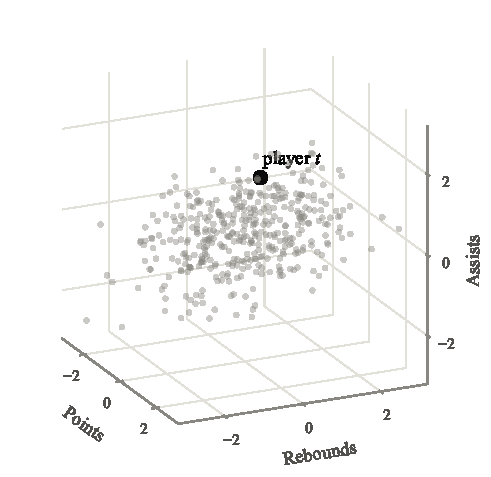
\includegraphics[width=0.45\linewidth]{basketball_cloud.pdf}
    \caption{\textbf{Players as points.} Each point is one of 400 simulated
    players, plotted at its points, rebounds and assists per game, in
    standard deviations from the average. Player $t$ is the example from
    the text.}
    \label{fig:bball-cloud}
\end{figure}
Figure~\ref{fig:bball-cloud} shows that these points form a cloud. This cloud is stretched based on correlation, and it's most stretched in the direction where all three variables rise together. 

PCA defines direction as a vector of weights $v=(v[1],\dots,v[N])$ of length one, $\sum_i v[i]^2=1$. 
How far player $t$ lies along that direction is the player's \emph{score}:
\[
s_t=v^\top x_t=\sum_{i=1}^{N}v[i]\,x_{i,t}.
\]
\begin{figure}[!htbp]
    \centering
    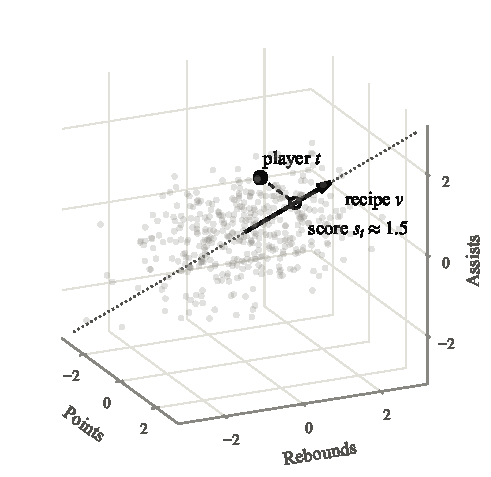
\includegraphics[width=0.55\linewidth]{basketball_recipe.pdf}
    \caption{\textbf{A recipe and a score.} The arrow is the recipe
    $v=(1,1,1)/\sqrt3$, which weights the three statistics equally.
    Dropping player $t$ straight onto the dotted line through it gives
    his score, $s_t\approx1.5$.}
    \label{fig:bball-recipe}
\end{figure}
The direction in Figure~\ref{fig:bball-recipe} is arbitrary. PCA finds the directions (eigenvectors) of the covariance matrix that maximize the spread of player scores along it, which we call "principal components." 

The spread of the cloud along $v$ is the variance of the scores across players, 
\[
\operatorname{Var}(s_t)=v^\top\Sigma v,
\]
where $\Sigma$ is the $N\times N$ covariance matrix of the statistics. Because the statistics are standardized, $\Sigma$ is also their correlation matrix.
The first principal component is the recipe with the most spread:
\[
\max_{v}\; v^\top\Sigma v \quad\text{subject to}\quad v^\top v=1 .
\]
Setting the derivative of the Lagrangian $v^\top\Sigma v-\lambda(v^\top
v-1)$ to zero gives
\[
\Sigma v=\lambda v .
\]
Multiplying both sides by $v^\top$ gives 

\[
v^\top\Sigma v=\lambda .
\]
This process gives us the cloud's eigenvectors (and their corresponding eigenvalues):
\begin{figure}[!htbp]
    \centering
    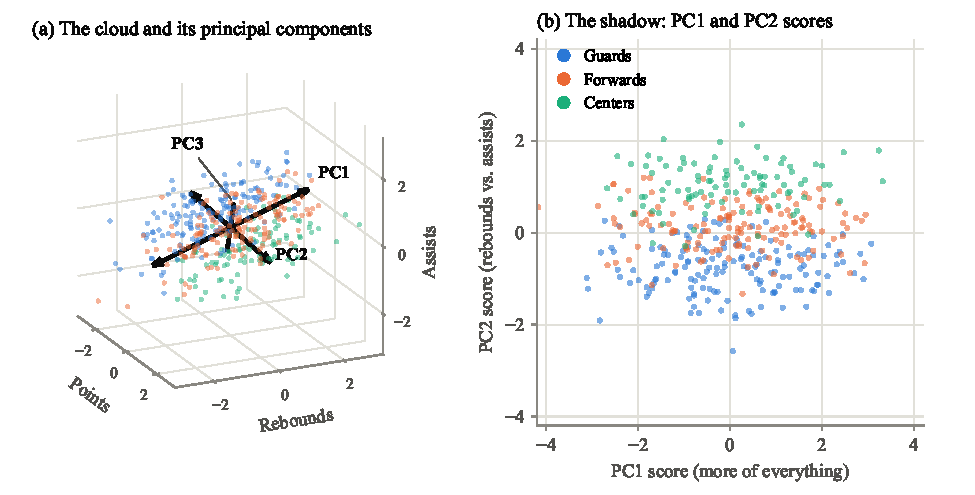
\includegraphics[width=\linewidth]{basketball_axes.pdf}
    \caption{\textbf{The principal components of the cloud.} (a) The
    three principal components, each spanning two standard deviations of
    spread on either side of the average player. Colors mark each
    simulated player's position, which PCA was not given. (b) Each
    player's PC1 and PC2 scores: the cloud viewed straight down PC3, the
    direction with the least spread.}
    \label{fig:bball-axes}
\end{figure}
By convention, we name principal components in decreasing order of their eigenvalues. PC1 is the eigenvector with the largest eigenvalue, PC2 is the orthogonal eigenvector with the most remaining spread among those whose scores are uncorrelated with PC1's, and so on, which you can see in Figure~\ref{fig:bball-axes}. 
We interpret these components by looking at their weights (called \emph{loadings} in PCA):
\[
v_1=(0.66,\,0.53,\,0.53),\qquad
v_2=(0.00,\,0.71,\,-0.71),\qquad
v_3=(0.75,\,-0.46,\,-0.47),
\]
with eigenvalues $\lambda_1=2.03$, $\lambda_2=0.75$ and $\lambda_3=0.21$.
Since all of PC1's loadings are positive, players with a high PC1 score are above average in points/rebounds/assists. This pattern likely reflects "minutes played." PC2 ignores points, weights rebounds positively, and assists negatively, so players with a high PC2 score rebound a lot but don't pass often, which is typical of centers; low PC2 players are the opposite, typical of guards (Figure~\ref{fig:bball-axes}b lets us see this more easily). 
% Page break removed; allow natural pagination.
The eigenvalues say how much each component "matters." After standardization, each statistic has variance 1, so the total variance of the cloud is $N = 3$, which the eigenvalues sum to. Each component's share of the total variance is $\lambda_k/N$, meaning PC1 explains $68\%$ of how players differ, PC2 $25\%$, and PC3 $7\%$. Because PC3 represents such a small relative share, we are probably able to drop it and not lose much information. This is how PCA enables \emph{dimensionality reduction}—if we had dozens of variables in our data as opposed to just three, we'd only have to keep a small share of components and we'd lose very little. 

Nothing here depends on having three statistics. With $N$ variables, each
observation is a point in $N$-dimensional space, $\Sigma$ is an $N\times N$
matrix, and the same maximization gives $N$ eigenvectors, each a list of $N$
loadings, with eigenvalues that add up to $N$. We can no longer draw the
cloud once $N>3$, but the math and the interpretation are unchanged. Each
principal component is still the direction of greatest remaining spread, its
eigenvalue is still how much spread it captures, and keeping only the first
$K$ components still compresses $N$ numbers into $K$. In our stock data, the
``players'' become trading days and the ``statistics'' become 1,201 stocks,
so each day is a point in 1,201 dimensions. Section~\ref{sec:stock-pca}
applies the same steps to that cloud.
\subsection{PCA on our stock returns}
\label{sec:stock-pca}
In the dataset we later analyze in our report, our variables are stocks where $N = 1201$, and our observations are trading days where $T = 6037$. Each day is a point in $1201$ dimensions, and the directions in which the cloud is stretched represent patterns of correlated stock movement.

To perform PCA on this dataset, we first standardize returns like we did before. The rationale is that if  "Stock A" was twice as volatile as "Stock B" but both had very correlated movement, A would dominate the loadings in PCA just because its swings are bigger. We standardize with 
\[
z_{i,t}=\frac{r_{i,t}-\bar{r}_i}{\bar{\sigma}_i}
\]
so each stock's return is mean zero and variance one (you might recognize these as "z-scores.") We then create a covariance matrix of standardized returns (= correlation matrix), which we'll call $C$:
\[
\operatorname{Cov}(z_i,z_j)=\frac{\operatorname{Cov}(r_i,r_j)}{\bar\sigma_i\,\bar\sigma_j}=\rho_{ij}.
\]
The principal components are thus the eigenvectors of the correlation matrix, $Cv=\lambda v$. To more easily visualize, we've picked out two utility stocks from our dataset, WEC Energy (WEC) and Duke Energy (DUK). Their daily returns have a correlation of $\rho=0.65$, so
\[
C=\begin{pmatrix}1&\rho\\ \rho&1\end{pmatrix},\qquad
v_1=\tfrac{1}{\sqrt2}\begin{pmatrix}1\\1\end{pmatrix},\ \lambda_1=1+\rho=1.65,
\qquad
v_2=\tfrac{1}{\sqrt2}\begin{pmatrix}1\\-1\end{pmatrix},\ \lambda_2=1-\rho=0.35.
\]

\begin{figure}[!htbp]
    \centering
    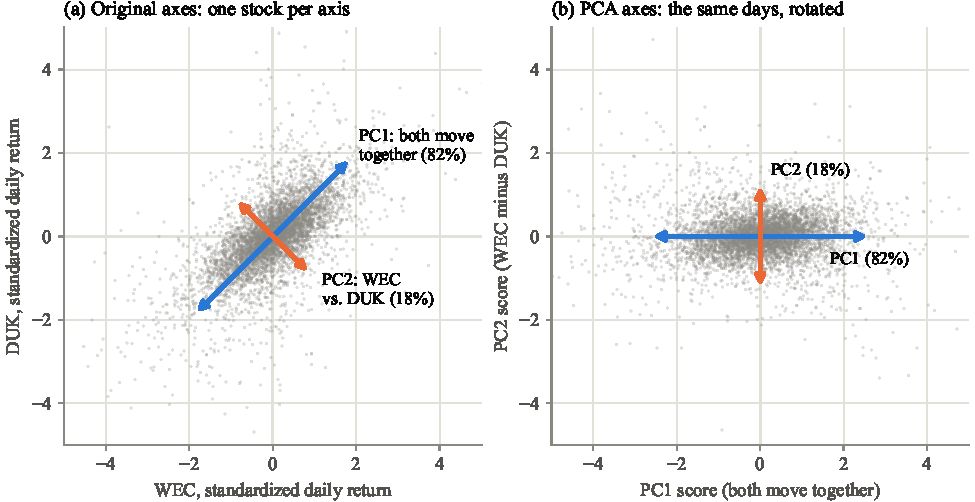
\includegraphics[width=\linewidth]{figures/primer_two_stocks.pdf}
    \caption{\textbf{PCA on two stocks.} Each point is one trading day
    from 2000 to 2023. (a) Standardized daily returns of WEC and DUK.
    The arrows are the two principal components, each spanning two
    standard deviations of spread on either side of zero. (b) The same
    days measured along the principal components. Percentages are
    shares of variance. Days with a move beyond five standard
    deviations (31 in panel a, 35 in panel b) lie outside the plotted range.}
    \label{fig:primer-two-stocks}
\end{figure}
If we add in two oil producers (Exxon Mobil/XOM and Occidental Petroleum/OXY), we can see how PCA starts to find broader trends:
\begin{table}[!htbp]
\centering
\caption{PCA run on four stocks alone: two utilities and two oil producers.}
\label{tab:primer-four}
\setlength{\tabcolsep}{5pt}
\begin{adjustbox}{max width=\linewidth}
\begin{tabular}{lrrrrrrl}
\toprule
& \multicolumn{4}{c}{Loadings $v_k[i]$} & & & \\
\cmidrule(lr){2-5}
Component & WEC & DUK & XOM & OXY & Eigenvalue & Share & Reads as \\
\midrule
PC1 & 0.48 & 0.49 & 0.54 & 0.49 & 2.322 & 58.1\% & All move together \\
PC2 & $-0.53$ & $-0.49$ & 0.41 & 0.56 & 1.065 & 26.6\% & Oil vs.\ utilities \\
PC3 & 0.70 & $-0.70$ & $-0.09$ & 0.12 & 0.351 & 8.8\% & WEC vs.\ DUK \\
PC4 & 0.03 & $-0.17$ & 0.73 & $-0.66$ & 0.262 & 6.5\% & XOM vs.\ OXY \\
\bottomrule
\end{tabular}
\end{adjustbox}
\\[4pt]
\small Daily returns, 2000--2023, standardized. 
\end{table}
From Table~\ref{tab:primer-four}, we might deduce that PC1 explains "general market movement," PC2 explains "sector-specific movement," and PC3/PC4 explain "sector-specific gaps" between industries. 
% Page break removed; allow natural pagination.
With all 1201 stocks, each trading day is a point in 1201 dimensions and each component is a list of 1201 loadings. This table would be too large to work with, so we've done PCA across the full sample and listed the first five principal components: 

\begin{table}[!htbp]
\centering
\caption{The first five principal components of all 1,201 stocks.}
\label{tab:primer-full}
\small
\setlength{\tabcolsep}{4pt}
\begin{adjustbox}{max width=\linewidth}
\begin{tabular}{lr >{\raggedright\arraybackslash}p{3.6cm} >{\raggedright\arraybackslash}p{3.6cm} >{\raggedright\arraybackslash}p{3.2cm}}
\toprule
Component & Share & Largest positive loadings & Largest negative loadings & Reads as \\
\midrule
PC1 & 26.7\% & SPY, MDY, DIA, XLI (index funds) & None: every loading is positive & The market \\
\addlinespace
PC2 & 2.9\% & VGM, NAD, VKQ, MYD (municipal bond funds) & STBA, CBU, WABC, NBTB (regional banks) & Rate-sensitive funds vs.\ banks \\
\addlinespace
PC3 & 2.0\% & ASML, LRCX, TXN, NVDA (semiconductors) & FRT, VNO, KIM, O (real estate) & Semiconductors vs.\ real estate \\
\addlinespace
PC4 & 1.6\% & ED, WEC, SO, DUK (utilities) & NBR, RIG, PTEN, DVN (oil drillers and services) & Defensive stocks vs.\ oil \\
\addlinespace
PC5 & 1.4\% & XOM, EOG, OXY, DVN (oil producers) & VTN, NAD, VGM, MYD (municipal bond funds) & Oil vs.\ bonds \\
\bottomrule
\end{tabular}
\end{adjustbox}
\\[4pt]
\small Full-sample PCA on standardized daily returns, 2000--2023. Each
component is oriented so its largest loading is positive, as in Q2.
\end{table}
The main difference from basketball is how much the components explain; before, PC1 and PC2 together explained $93\%$ of how players differ. On the full set of stocks, it takes 70 components to explain half of the variance (Q1). 
\subsection{From PCA to the factor model}
To trade on the components, and to split each stock's return into a
shared and an idiosyncratic part, the assignment turns them into
portfolios, factor returns and a regression. Questions 2--6 do this on
our data; here we explain what each step means.

\paragraph{Scores.} In stock terms, the loading $v_k[i]$ says how much
stock $i$ takes part in component $k$, and the score
$s_{k,t}=\sum_i v_k[i]\,z_{i,t}$ says how strongly component $k$ showed up
on day $t$. A high PC1 score is a day when most stocks rose; a high PC3
score is a day when technology beat real estate.

\paragraph{Eigenportfolios (Q2).} A loading is a weight on a
\emph{standardized} return, not a dollar amount. To hold a component as a
portfolio, we divide each loading by the stock's standard deviation and
scale so the absolute weights add up to one:
\[
w_{k,i}=\frac{v_k[i]/\bar\sigma_i}{\sum_{j}\left|v_k[j]/\bar\sigma_j\right|}.
\]
Positive weights are long positions and negative weights are short
positions, and $\sum_i|w_{k,i}|=1$ means one dollar of gross exposure per
dollar of capital. This is an \emph{eigenportfolio}.
Table~\ref{tab:primer-vol} shows why we divide by the standard deviation:
a stock twice as volatile gets half the dollars, so on a day when every
stock moves one standard deviation, each contributes equally, just as in
the PCA.

\begin{table}[!htbp]
\centering
\caption{Same loading, different volatility (illustrative).}
\label{tab:primer-vol}
\begin{adjustbox}{max width=\linewidth}
\begin{tabular}{lrrrrr}
\toprule
Stock & Loading $v$ & Daily $\bar\sigma$ & $v/\bar\sigma$ & Share of gross & Contribution on a $+1\bar\sigma$ day \\
\midrule
X & 0.58 & 1.0\% & 0.58 & 46\% & $0.58\times1.0=0.58$ \\
Y & 0.58 & 2.0\% & 0.29 & 23\% & $0.29\times2.0=0.58$ \\
Z & 0.58 & 1.5\% & 0.39 & 31\% & $0.39\times1.5=0.58$ \\
\bottomrule
\end{tabular}
\end{adjustbox}
\end{table}

\paragraph{Factor returns (Q3).} A factor's return is how its
eigenportfolio did on a given day:
\[
f^k_t=\sum_{i=1}^{N}\frac{v_k[i]}{\bar\sigma_i}\,r_{i,t}
=s_{k,t}+\sum_{i=1}^{N}\frac{v_k[i]\,\bar r_i}{\bar\sigma_i}.
\]
It is the PCA score in return units plus a constant, so factor returns
are uncorrelated with each other over the estimation sample, as Q3
confirms. Q2's rescaling to one dollar of gross exposure only multiplies
each factor return by a constant.

\paragraph{Betas, alpha and residuals (Q5).} Regressing each stock's
return on the factor returns,
\[
r_{i,t}=\alpha_i+\sum_{k=1}^{K}\beta_{k,i}f^k_t+\varepsilon_{i,t},
\]
gives its \emph{betas} $\beta_{k,i}$, how strongly it moves with each
factor; its \emph{alpha} $\alpha_i$, the part of its average return the
factors do not explain; and its \emph{residuals} $\varepsilon_{i,t}$, the
stock-specific surprise each day, whose variance $\sigma^2(\varepsilon_i)$
is its idiosyncratic risk. Alphas are tiny next to daily noise: Q5 finds a
median of 0.3 basis points per day.

\paragraph{The shared part and the idiosyncratic part.} Since the
eigenvectors are perpendicular with length one, each standardized return
can be rebuilt exactly from all $N$ scores, and cutting the sum at $K$
splits it in two:
\[
z_{i,t}=
\underbrace{\sum_{k=1}^{K} v_k[i]\,s_{k,t}}_{\text{shared part}}
+\underbrace{\sum_{k=K+1}^{N} v_k[i]\,s_{k,t}}_{\text{idiosyncratic part}} .
\]
The regression makes the same split in return units: over the full
sample, $\beta_{k,i}=\bar\sigma_i\,v_k[i]$ and $\varepsilon_{i,t}$ is
$\bar\sigma_i$ times the idiosyncratic part. In basketball we dropped the
leftover as noise. With stocks, the leftover is what our strategies trade.

\paragraph{How this differs from standard factors (Q6).} Standard factor
models define factors first from economic rules, such as the market,
value and momentum, and then estimate each stock's exposure. PCA builds
factors from the data and we interpret them afterwards. Some match
familiar factors (PC1 the market, PC3 value) and some do not (PC2), as Q6
shows. PCA also finds what moves together, not what earns a premium:
explaining past variance is different from predicting future returns.

\subsection{Summary}
Table~\ref{tab:primer-map} lines up the two settings. PCA turns a cloud of
correlated data into uncorrelated directions, ranked by how much of the
spread each explains. The directions are the eigenvectors of the
correlation matrix, and the spread along each is its eigenvalue.

\begin{table}[!htbp]
\centering
\caption{The same PCA in two settings.}
\label{tab:primer-map}
\small
\begin{adjustbox}{max width=\linewidth}
\begin{tabular}{>{\raggedright\arraybackslash}p{3.4cm} >{\raggedright\arraybackslash}p{5.2cm} >{\raggedright\arraybackslash}p{5.6cm}}
\toprule
& Basketball & Stocks \\
\midrule
A point in the cloud & A player & A trading day \\
An axis & A statistic ($N=3$) & A stock ($N=1{,}201$) \\
Standardizing & Each statistic in standard deviations from the league average & Each stock's return in standard deviations from its own mean \\
Loading $v_k[i]$ & How much a statistic counts in a component & How much a stock takes part in a component \\
Score $s_{k,t}$ & A player's one-number summary & A day's factor return (Q3), up to a constant \\
PC1 & Volume, mostly minutes played & The market (Q4) \\
Later PCs & Position: centers vs.\ point guards & Sectors and themes \\
Top components explain & 93\% with $K=2$ & 35\% with $K=5$ \\
Turned into a trade & Not applicable & An eigenportfolio (Q2); betas measure each stock's exposure (Q5) \\
The leftover & Mostly noise, dropped & The idiosyncratic part, traded \\
\bottomrule
\end{tabular}
\end{adjustbox}
\end{table}

For basketball, two components describe players almost completely. For
stocks, the first component is the market and the next few are sectors
and themes, but together they explain only about a third of daily
movement. That is what makes PCA useful for trading: it lets us strip the
shared part out of each stock's return and look at what is left. The
answers to Questions 1--6 below carry out each step on our data.
Section~\ref{sec:framework} describes how we estimate the model as time moves forward
without using future information, and Section~\ref{sec:strategies} builds three strategies
on the idiosyncratic part.



% Page break removed; allow natural pagination.
\section{PCA results: Questions 1--6}
\begin{enumerate}
\item Using stock returns at the daily (or monthly) level, perform a principal
component analysis (PCA) on daily (monthly) stock returns. Feel free to refer
to online resources. How many factors are needed to explain a reasonable
proportion of the total variance in stock returns? (There is no right answer
to this, although there are standard share of variance measures that are
some diagnostic tests). (\emph{Hint:} what preprocessing should you do
before performing a PCA, and why?)

\answer
We performed principal component analysis (PCA) on daily returns for
1,201 stocks over 6,037 trading days from January 3, 2000, through
December 29, 2023. Before fitting PCA, we subtracted each stock's sample
mean and divided by its sample standard deviation. This gives each
stock unit variance and is equivalent to performing PCA on the return
correlation matrix.

Figure~\ref{fig:q1-explained-variance} shows a sharp drop after the
first principal component. PC1 explains 26.70\% of standardized return
variance, and the first five components explain \textbf{34.63\%}.
Components two through five add 7.93 percentage points combined.
We use five factors as a compact summary of the largest patterns in
returns. If the goal is to explain at least half of standardized return
variance, we need \textbf{70 components}. The number rises to 278 for
70\% and 672 for 90\%.

To see how preprocessing affects the leading component, we repeated
PCA on centered raw returns using the same stocks and dates. The 240
most volatile stocks accounted for 28.04\% of PC1's squared loadings
before standardization and 10.67\% afterward. If squared loadings were
distributed evenly across stocks, this group would account for 20.0\%.
Standardization therefore reduced the concentration of PC1's loadings
among the most volatile stocks in our sample. We use the standardized
fit for our main results to identify shared movements across stocks on
a common volatility scale.

\begin{figure}[!htbp]
    \centering
    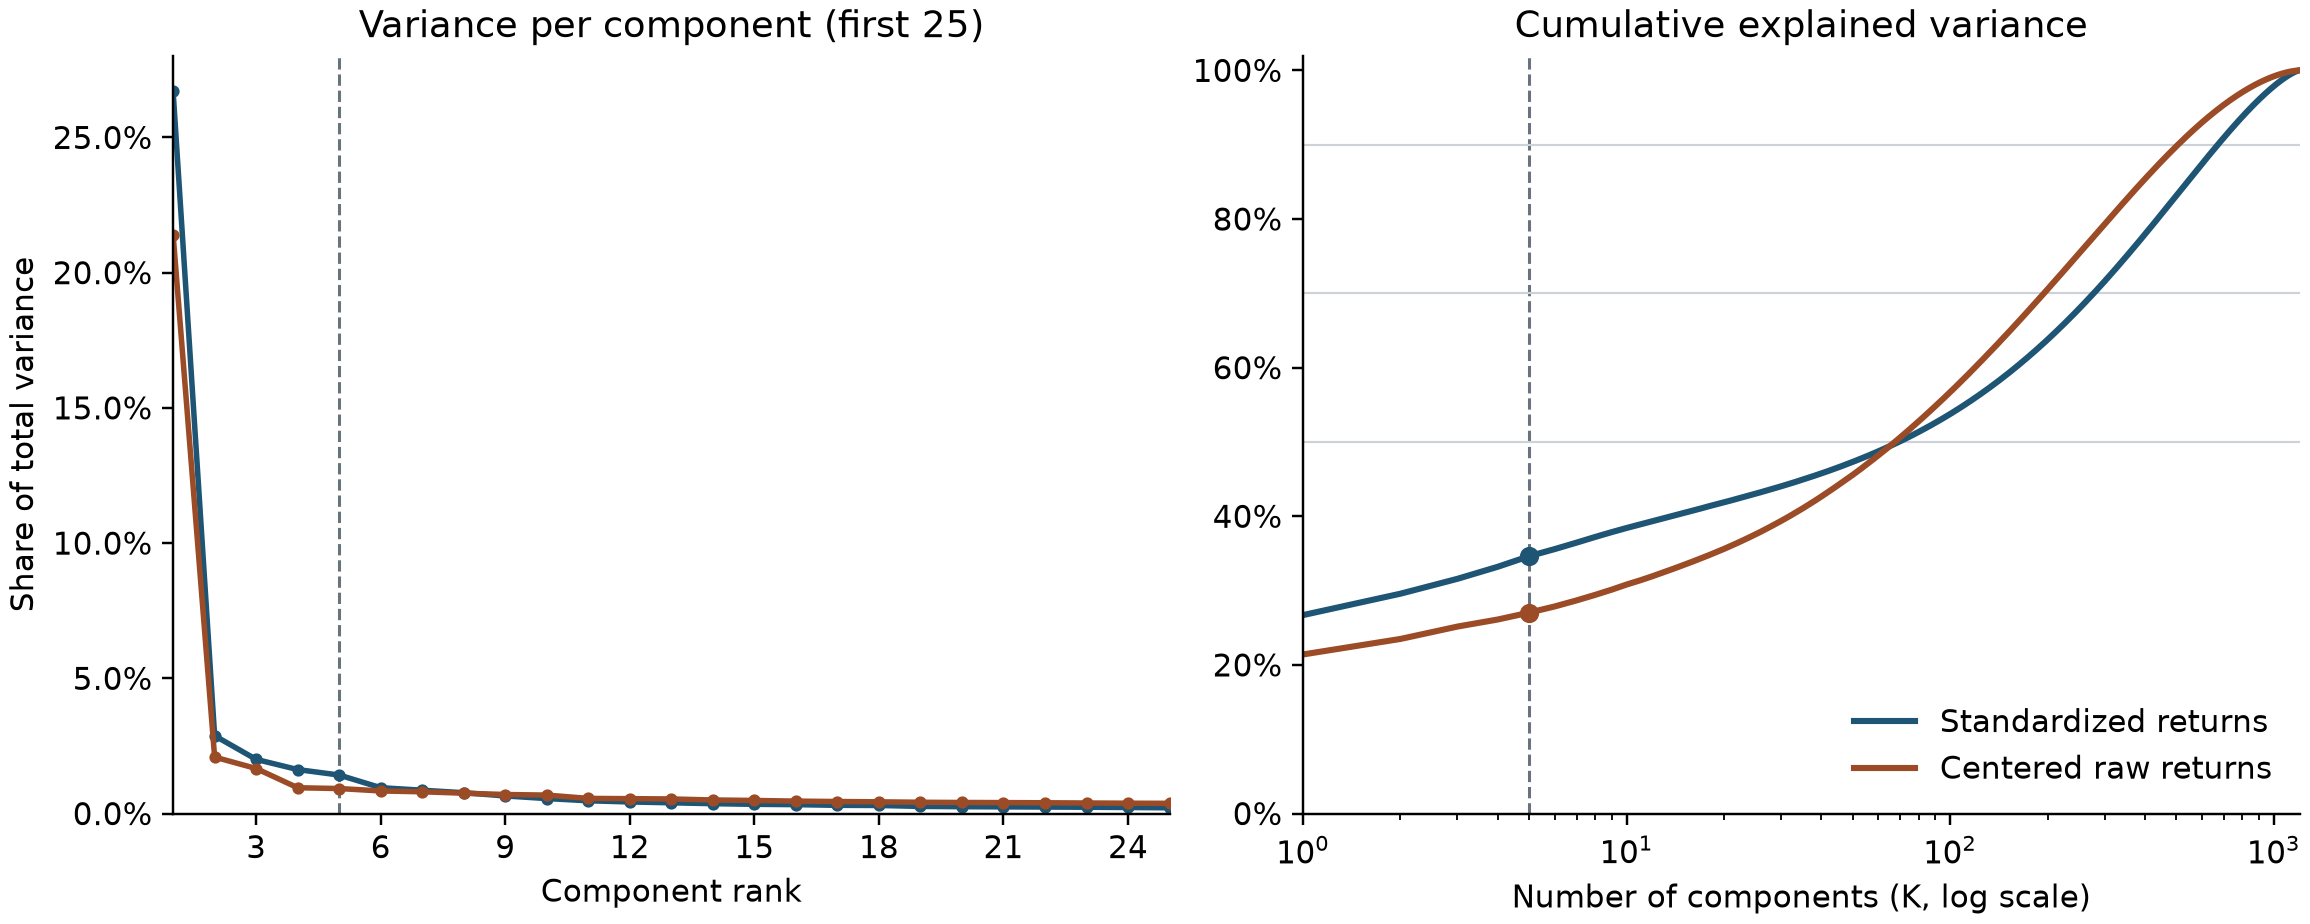
\includegraphics[width=0.85\linewidth]{figures/q1_explained_variance.png}
    \caption{\textbf{Explained variance from PCA on daily stock returns.}
    The left panel shows the share of variance explained by each of the
    first 25 principal components. The right panel shows cumulative
    explained variance, with the number of components on a logarithmic
    scale. The dashed vertical line marks \(K=5\), which explains
    34.63\% of the variance in standardized returns and 27.04\% in
    centered raw returns. Both fits use the same stocks and dates.}
    \label{fig:q1-explained-variance}
\end{figure}

\item Let's focus on a low number of factors: $K=5$. Compute (based on the total
sample for now) the $K=5$ principal components.

\begin{itemize}
\item Each principal component should be a vector of length $N$, the number
of stocks in your universe. How can one translate a principal component vector
$v_k$ into a tradable portfolio? (\emph{Hint:} what should you do with the
vector elements?)
\end{itemize}

\answer
We retain the five eigenvectors associated with the largest eigenvalues
of the full-sample return correlation matrix. Each eigenvector \(v_k\)
has 1,201 entries, one per stock. Together, the five components explain
34.63\% of standardized return variance.

To turn each component into an eigenportfolio, we divide each
coefficient \(v_k[i]\) by the stock's sample return standard deviation
\(\bar{\sigma}_i\). We then scale the resulting weights to one dollar
of gross exposure per dollar of capital:
\[
w_{k,i}
=
\frac{v_k[i]/\bar{\sigma}_i}
     {\displaystyle\sum_{j=1}^{1{,}201}
      \left|v_k[j]/\bar{\sigma}_j\right|}.
\]
Positive weights represent long positions, and negative weights represent
short positions. We orient each component so that its largest coefficient
in absolute value is positive. This fixes the sign convention for the
long and short positions shown in Figure~\ref{fig:q2-eigenportfolios}.

PC1 explains 26.70\% of standardized return variance and produces an
effectively long-only portfolio. Its ten largest positions account for
just 2.57\% of gross exposure, the lowest share among the five portfolios.
PC2 explains only 2.88\% of standardized variance, yet its ten largest
positions account for 9.32\% of gross exposure, the highest share of
the five. Under our sign convention, PC2 has a net long exposure of
51.3\%, while PC3 and PC5 have smaller net short exposures of 7.0\%
and 8.8\%, respectively.

The inverse-volatility adjustment also changes which stocks receive
the largest positions. For PC2 and PC5, only two of the ten stocks with
the largest absolute PCA coefficients remain in the top ten after the
adjustment. For PC1 and PC4, seven of ten remain. A stock can therefore
be prominent in the standardized component and receive a smaller
position in the eigenportfolio because of its return volatility.

\begin{figure}[!htbp]
    \centering
    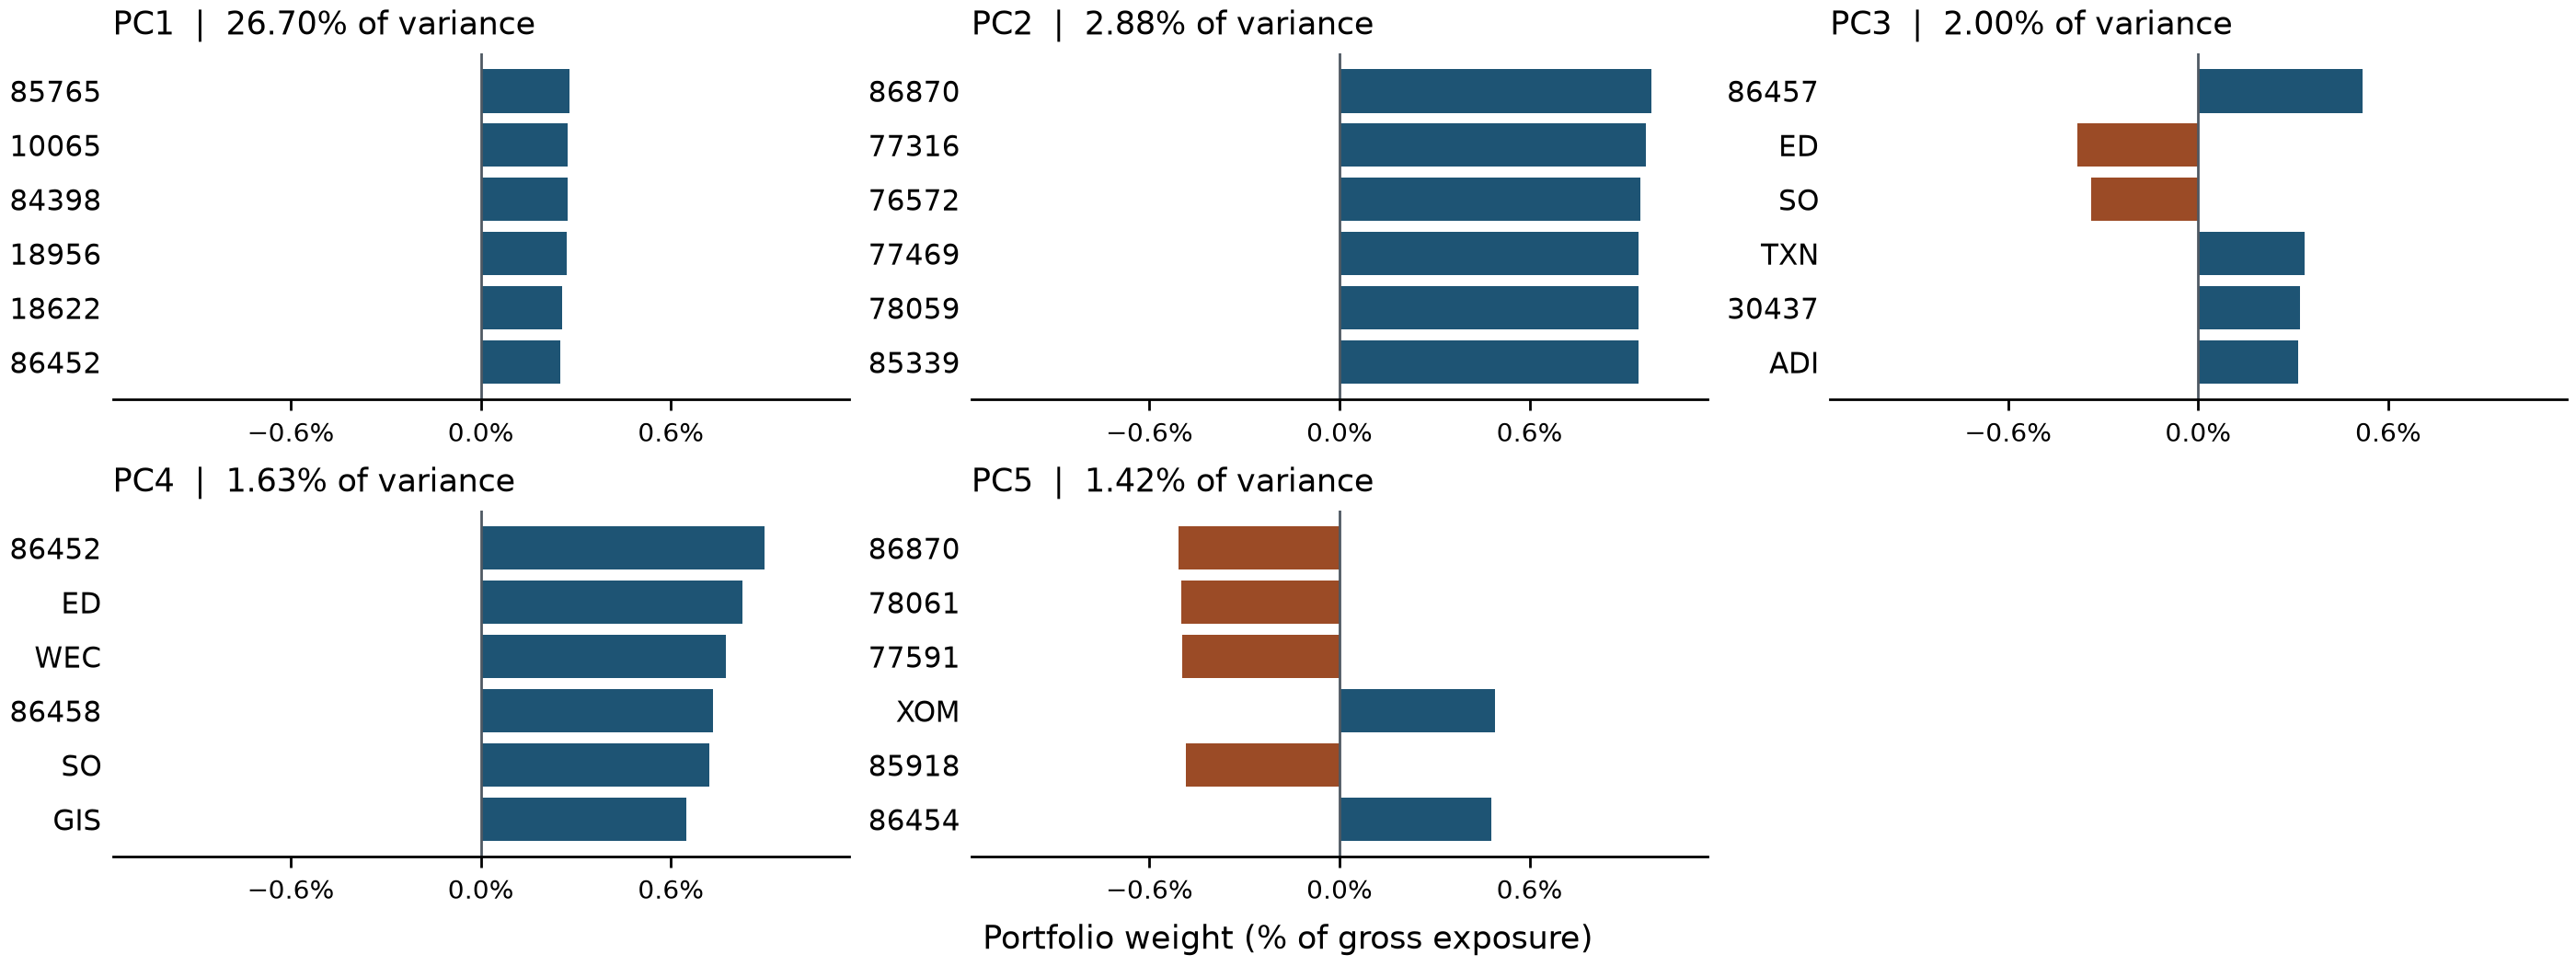
\includegraphics[width=0.85\linewidth]{figures/q2_eigenportfolios.png}
    \caption{\textbf{Largest positions in the five PCA eigenportfolios.}
    Each panel shows the six largest positions by absolute weight on a
    common scale. Positive and negative bars indicate long and short
    positions. Numeric labels are stock IDs. Panel titles report each
    component's share of standardized return variance.}
    \label{fig:q2-eigenportfolios}
\end{figure}


\item For each principal component vector $v_k$, compute the factor returns
for the eigenportfolio
$f_t^k=\sum_i\frac{v_k[i]}{\bar\sigma_i}\cdot r_{i,t}$, where
$\bar\sigma_i$ is the standard deviation for stock $i$ returns. Why do we
want to normalize the $v_k$ by the standard deviation?

\answer
Using the five full-sample eigenvectors from Q2, we compute daily factor
returns for all 6,037 trading days:
\[
f_t^k =
\sum_{i=1}^{1{,}201}
\frac{v_k[i]}{\bar{\sigma}_i}\,r_{i,t},
\qquad k=1,\ldots,5.
\]
We use the scaling specified in Q3. Applying Q2's gross-exposure
normalization would multiply each factor series by a constant.

We divide each coefficient by the stock's standard deviation because
the eigenvectors were estimated on standardized returns. For example,
if two stocks have the same PCA coefficient and one is twice as volatile,
the more volatile stock receives half the raw-return weight. A
one-standard-deviation move in either stock then makes the same
contribution to the factor.

The scaling also preserves the original PCA scores up to a constant.
If \(\bar r_i\) is stock \(i\)'s sample mean, then
\[
f_t^k-\bar f^k =
\sum_{i=1}^{1{,}201}
v_k[i]\frac{r_{i,t}-\bar r_i}{\bar{\sigma}_i}.
\]
The right-hand side is the PCA score, so the factor returns are
uncorrelated over the full estimation sample. In our data, applying the
eigenvector coefficients directly to raw returns gives a largest
absolute pairwise correlation of \textbf{0.5672}. Dividing by each
stock's standard deviation brings that value to \textbf{zero up to
numerical precision}.

Figure~\ref{fig:q3-factor-volatility} shows that factor volatility
varies even with fixed weights. PC1's 63-day volatility reached
67.25 factor units in December 2008, about 3.8 times its full-sample
daily standard deviation of 17.91. PC2 and PC5 also peaked in December
2008, while PC4 peaked in May 2020. These values are in factor units
under the scaling above.

\begin{figure}[!htbp]
    \centering
    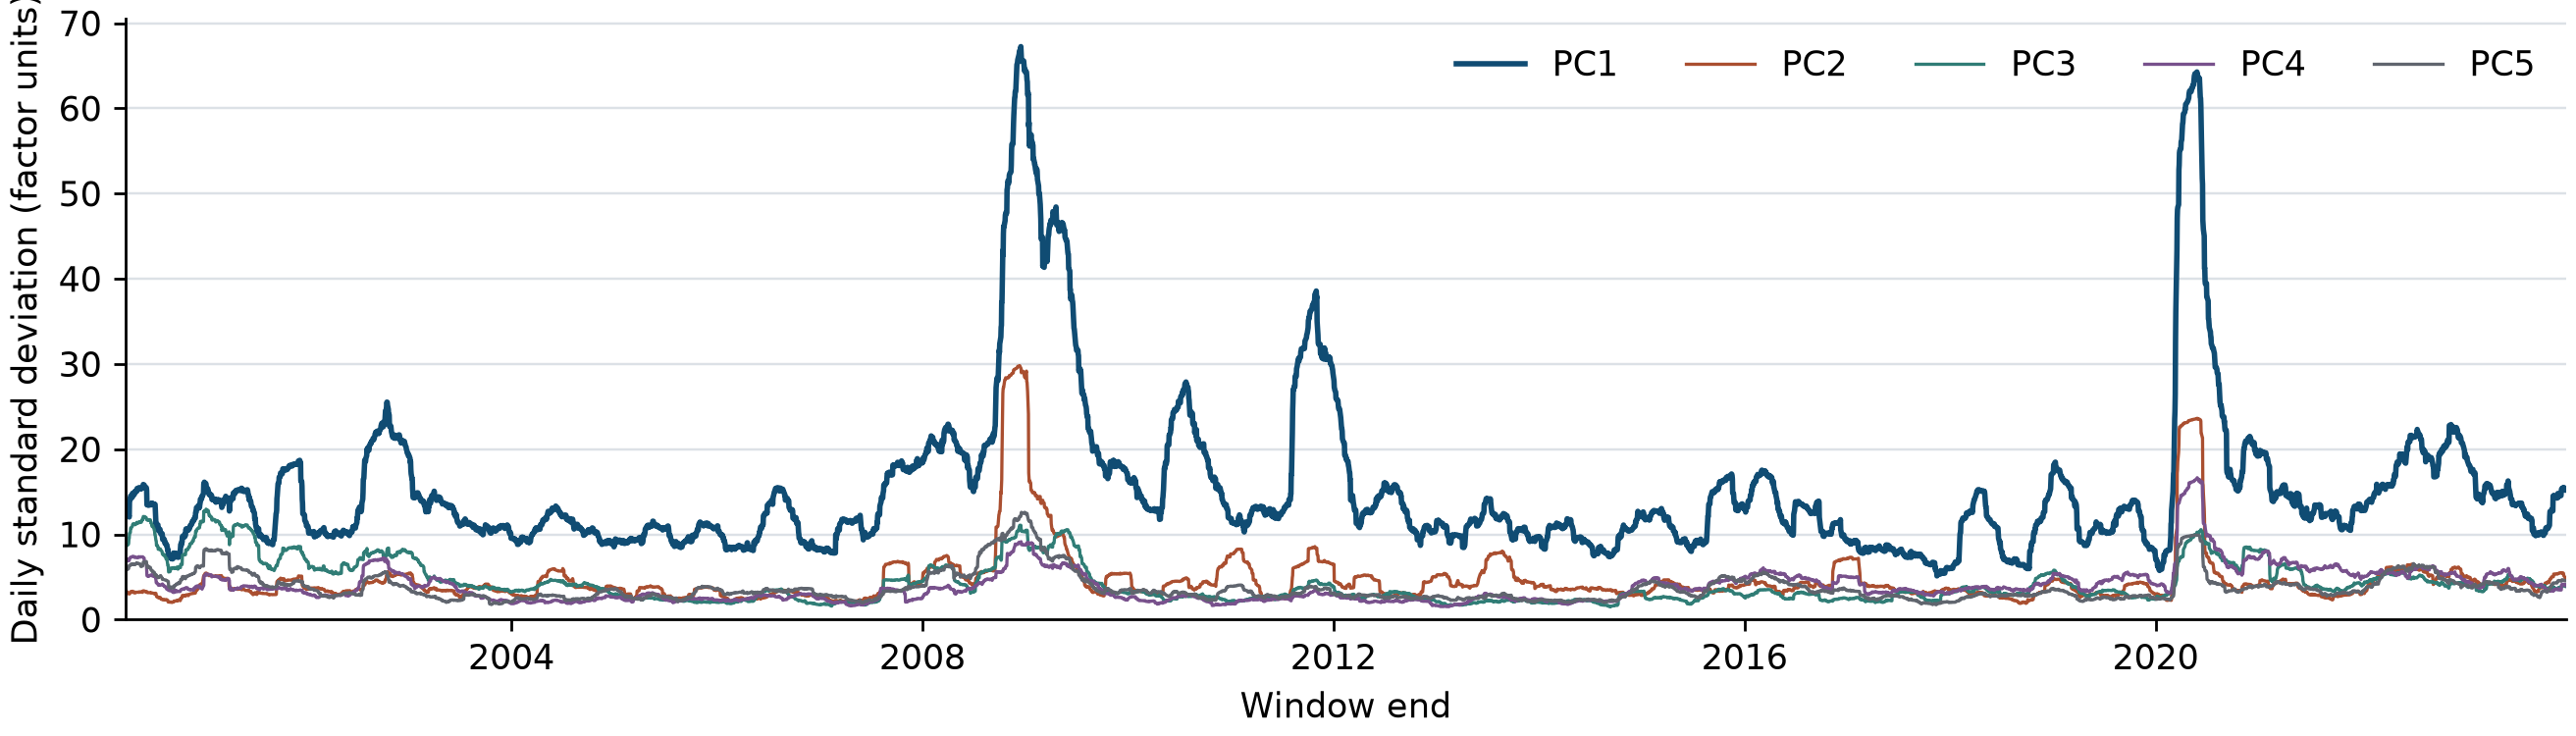
\includegraphics[width=0.85\linewidth]{figures/q3_factor_volatility.png}
    \caption{\textbf{Rolling volatility of the five PCA factor returns.}
    Each line shows the standard deviation of daily factor returns
    over the 63 trading days ending on the plotted date. The
    full-sample factor weights are fixed throughout.}
    \label{fig:q3-factor-volatility}
\end{figure}


\item Focus on the first factor return: what's the correlation of that with
respect to market returns?

\answer
We compare the first PCA factor with the daily value-weighted U.S.
market return from the
\href{https://mba.tuck.dartmouth.edu/pages/faculty/ken.french/data_library.html}
{Kenneth French Data Library}. We add the reported risk-free rate to
the market excess return to recover the total market return. The two
series match on all 6,037 trading days from January 3, 2000, through
December 29, 2023.

Under the sign convention used in Q2, the full-sample Pearson
correlation is \textbf{\(r=0.9373\)}. Regressing PC1 on the market
return with an intercept gives an \(R^2\) of 0.8785, so the market
return accounts for 87.85\% of PC1's daily variation in this regression.
This strong positive relationship is consistent with Q2's finding that
PC1 is an effectively long-only portfolio with weights spread across
many stocks.

Figure~\ref{fig:q4-pc1-market} shows that the strength of this
relationship varies over time. The trailing 252-trading-day correlation
has a median of 0.9623 and ranges from 0.7310 to 0.9898. The minimum
occurs in the window ending July 7, 2021, when PC1 tracked the broad
market substantially less closely than it did over the full sample.

\begin{figure}[!htbp]
    \centering
    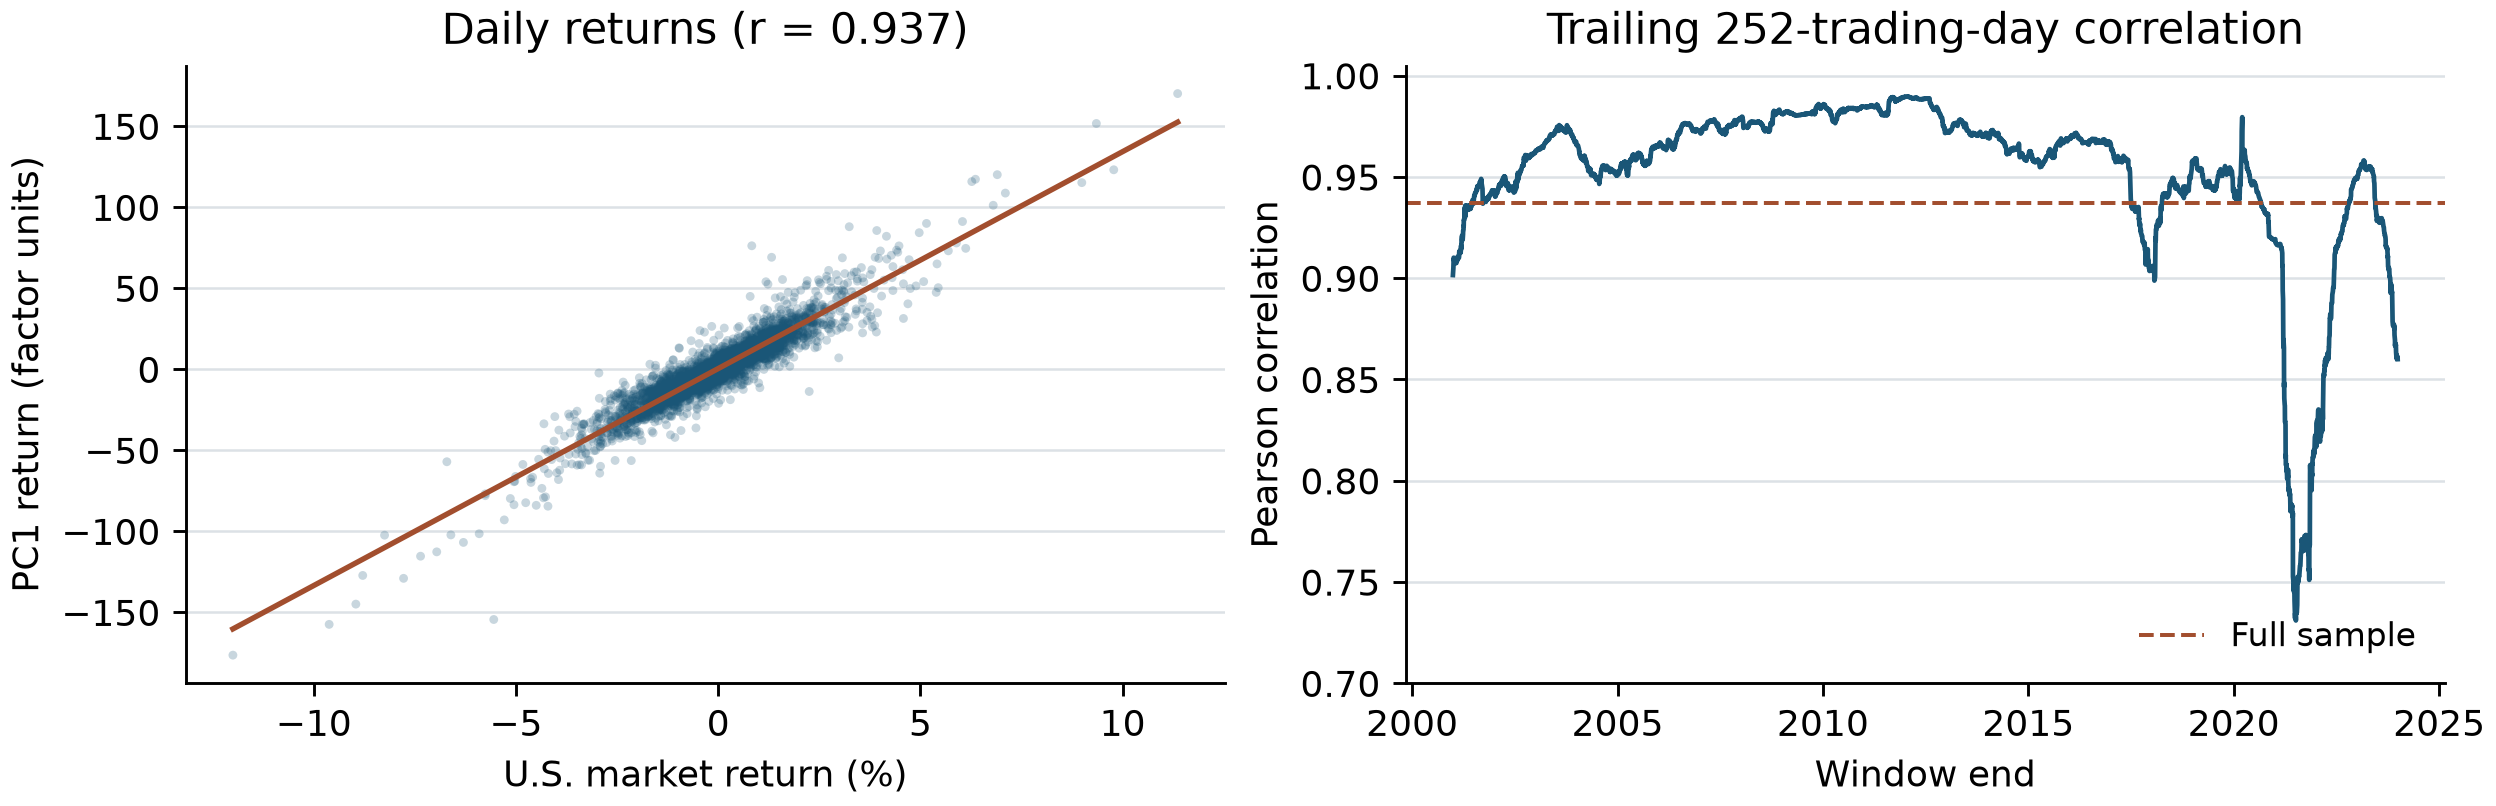
\includegraphics[width=0.85\linewidth]{figures/q4_pc1_market.png}
    \caption{\textbf{PC1 and the U.S. market return.}
    The left panel shows matched daily returns and the fitted
    regression line. The right panel shows trailing 252-trading-day
    Pearson correlations. The dashed line marks the full-sample
    correlation.}
    \label{fig:q4-pc1-market}
\end{figure}

\item For each stock \(i\), run the regression
\(r_{i,t}=\alpha_i+\sum_k\beta_{k,i}f_t^k+\epsilon_{i,t}\).
What is the interpretation of \(\alpha_i\)?

\answer
We regress each of the 1,201 stocks' daily returns on the five
PCA factor returns from Q3 over 6,037 trading days. The intercept
\(\alpha_i\) is the stock's fitted daily return when all five factor
returns are zero. Because the regression includes an intercept,
\[
\hat{\alpha}_i
=
\bar r_i-\sum_{k=1}^{5}\hat{\beta}_{k,i}\bar f^k.
\]
Thus, a positive alpha means the stock earned more on average than
the model attributes to its factor exposures. The residual
\(\hat{\epsilon}_{i,t}\) is the difference between the stock's actual
and fitted return on a particular day.

The median estimated alpha is \(0.298\) basis points per day, with
5th and 95th percentiles of \(-3.303\) and \(6.932\), respectively.
The median stock-level in-sample \(R^2\) is 0.3536.
In Figure~\ref{fig:q5-stock-alphas}, every stock lies below the
diagonal, meaning the fitted factor contributions were positive
on average for every stock. The median gap between mean return
and estimated alpha is \(5.846\) basis points per day.

The raw-return and alpha rankings have a Spearman correlation of
0.7264. Of the 240 stocks in the top quintile by raw average return,
\textbf{162 remain in the top quintile by alpha}. The factor
adjustment therefore changes 78 of the 240 names that a
top-quintile strategy would select. These estimates describe the
full sample. The out-of-sample backtest tests whether the alpha
ranking predicts future returns.

\begin{figure}[!htbp]
    \centering
    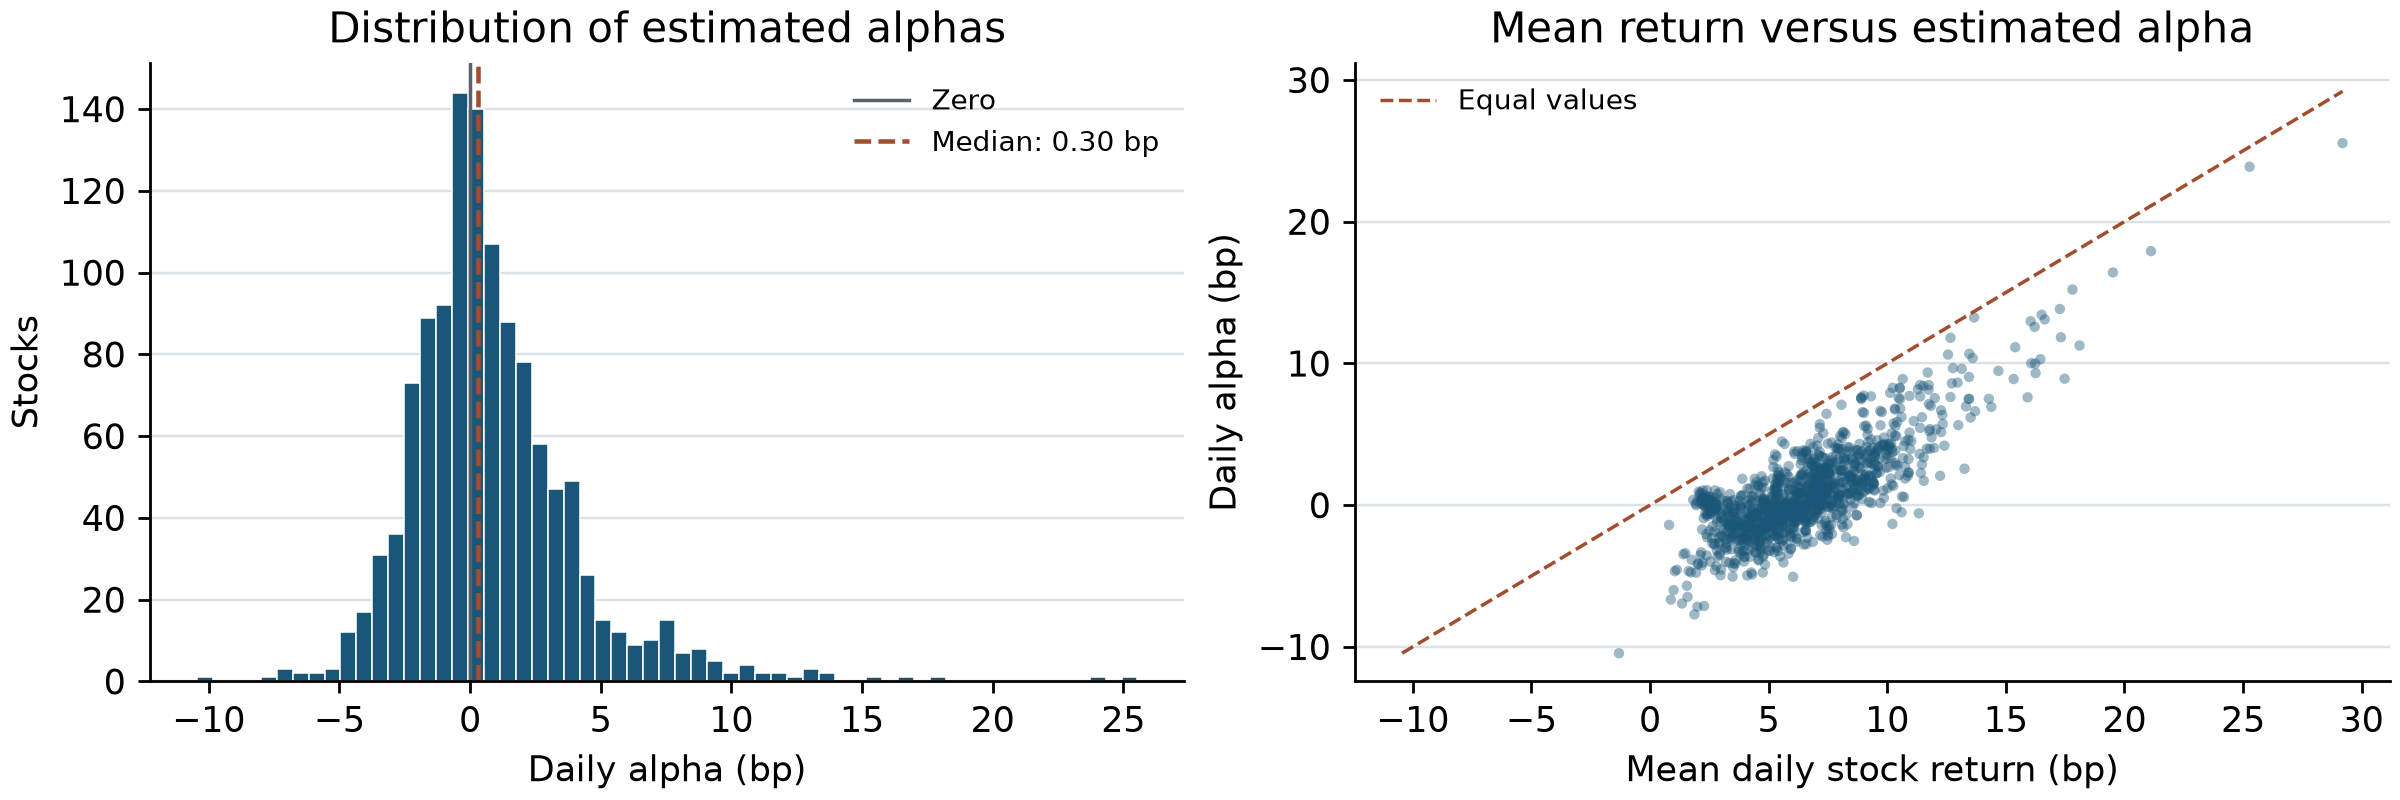
\includegraphics[width=0.85\linewidth]{figures/q5_stock_alphas.png}
    \caption{\textbf{Estimated daily stock alphas.}
    The left panel shows the distribution of estimated alphas.
    The right panel plots each stock's estimated alpha against its
    mean daily return. The dashed diagonal marks equal values.
    Both return measures are in basis points per day.}
    \label{fig:q5-stock-alphas}
\end{figure}


\item How does this approach differ from standard factors
(i.e.\ using market, value, momentum)?

\answer
Standard factors are defined by portfolio construction rules. The
market factor is the broad market return minus the risk-free rate.
Value (HML) measures the return spread between stocks with high and
low book-to-market ratios, while momentum (Mom) measures the spread
between stocks with high and low past returns. PCA instead estimates
its factors directly from stock returns. It selects orthogonal
directions that explain as much in-sample variation in standardized
returns as possible. The economic interpretation comes after estimation.

We match the five PCA factors to daily market excess, value, and
momentum returns from the
\href{https://mba.tuck.dartmouth.edu/pages/faculty/ken.french/data_library.html}
{Kenneth French Data Library} on all 6,037 trading days. We compute
pairwise Pearson correlations and regress each PCA factor jointly on
the three standard factors with an intercept. We use the market
excess return here and the total market return in Q4.

Figure~\ref{fig:q6-pca-vs-standard-factors} shows that PC1 has a
correlation of \(0.9372\) with the market excess return. The three
standard factors jointly explain about 93.4\% of PC1's daily
variation, roughly 5.6 percentage points more than the market
excess return alone. Under our sign convention, PC3 has a
\(-0.6022\) correlation with HML, the strongest absolute value
correlation among the five components.

PC2 explains 2.88\% of standardized stock return variance, the
second-largest share among the components. Yet market, value, and
momentum jointly explain only \textbf{0.69\% of PC2's daily
variation}. The corresponding figure for PC5 is 3.73\%.
These results show that some PCA factors closely track familiar
benchmarks, while others capture patterns in this stock universe
that the three standard factors explain very little of.

\begin{figure}[!htbp]
    \centering
    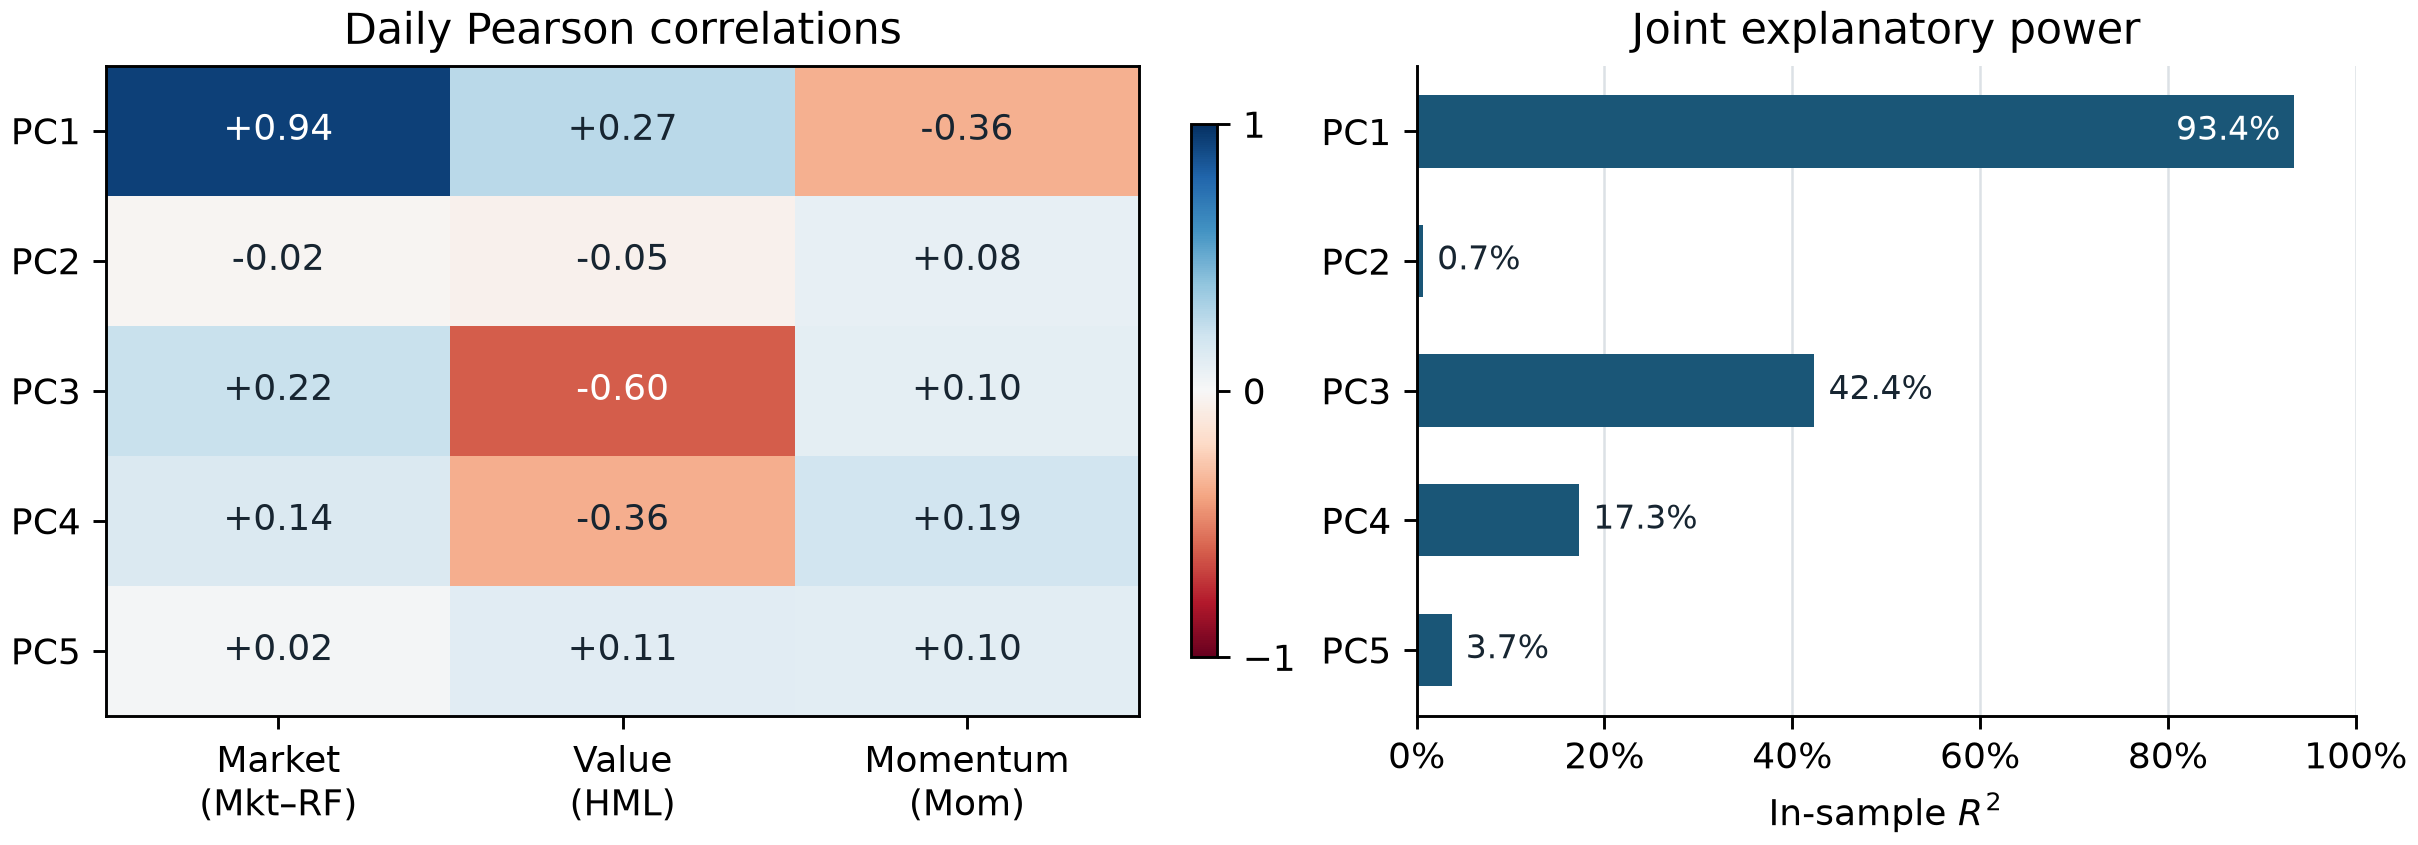
\includegraphics[width=0.85\linewidth]
        {figures/q6_pca_vs_standard_factors.png}
    \caption{\textbf{PCA factors and standard U.S. equity factors.}
    The left panel shows daily Pearson correlations. The right panel
    reports the in-sample \(R^2\) from regressing each PCA factor
    jointly on market excess, value, and momentum returns.}
    \label{fig:q6-pca-vs-standard-factors}
\end{figure}

% BEGIN ARCHIVED: Assignment prompts 7--12; answered in the following sections
% ARCHIVE \item Construct a trading strategy based on your estimate of $\alpha_i$.
% ARCHIVE If you are totally out of ideas, one thing would be to sort the stocks
% ARCHIVE based on your estimates of $\alpha_i$, go long stocks in the top quintile
% ARCHIVE of alpha, go short stocks in the bottom quintile of alpha. A trading
% ARCHIVE strategy should consist of how much of each stock $i$ to hold (can be
% ARCHIVE negative) at any point in time $t$. Note that if you put weights $w_{i,t}$
% ARCHIVE on stock $i$ at time $t$, your returns $r_{\mathrm{port},t+1}$ is given by
% ARCHIVE $\sum_i w_{i,t}\cdot r_{i,t+1}$.
% ARCHIVE 
% ARCHIVE \begin{itemize}
% ARCHIVE     \item Feel free to be more entrepreneurial/creative in this section.
% ARCHIVE     \item Make sure your trading strategy is not based on future returns,
% ARCHIVE     e.g.\ you go long stocks that will move up tomorrow.
% ARCHIVE \end{itemize}
% ARCHIVE 
% ARCHIVE \item Visualize / report the cumulative returns of the trading strategy.
% ARCHIVE Let $r_{\mathrm{port},t}$ be the returns of your trading strategy for
% ARCHIVE time $t$.
% ARCHIVE 
% ARCHIVE \item Compute the Sharpe ratio of your trading strategy.
% ARCHIVE 
% ARCHIVE \item Compute the information ratio of your trading strategy:
% ARCHIVE 
% ARCHIVE \begin{itemize}
% ARCHIVE     \item Formally, run the regression:
% ARCHIVE     $r_{\mathrm{port},t}=\alpha+\beta r_{\mathrm{mkt},t}$.
% ARCHIVE     Your reference return (for the information ratio) should be
% ARCHIVE     $\beta\cdot r_{\mathrm{mkt},t}$.
% ARCHIVE     \item Is your strategy market neutral?
% ARCHIVE \end{itemize}
% ARCHIVE 
% ARCHIVE \item Note that you have estimated the PCA using the entire sample.
% ARCHIVE Thus, your estimates of your trading performance should be somewhat
% ARCHIVE positively biased. Now, repeat your exercise, where you simulate a
% ARCHIVE trading strategy across time, where you a) estimate your factors only
% ARCHIVE based on data in the past (so at 2015 January, you construct your
% ARCHIVE PCAs using data up to 2015 January), and then construct a trading
% ARCHIVE strategy, and see how this strategy performs. A simple starting point
% ARCHIVE is to estimate $\alpha_i$s using data prior to 2015, and assume
% ARCHIVE $\alpha_i$s stay fixed afterwards. Of course, you can also update your
% ARCHIVE $\alpha_i$ estimates every day/month when you roll forward. Be very
% ARCHIVE clear how you avoided the look-ahead bias.
% ARCHIVE 
% ARCHIVE \item Why stop at $K=5$? Across multiple values of $K$, re-do all of
% ARCHIVE the above exercises. Which $K$ seems to work best? Is there a
% ARCHIVE significant difference between in-sample assessments (one where you
% ARCHIVE estimate the factors based on all the data) and out-sample assessments
% ARCHIVE (one where you estimate the factors only based on data available at
% ARCHIVE the time and roll forward)? Discuss.
% END ARCHIVED: Assignment prompts 7--12; answered in the following sections
\end{enumerate}

\begingroup\small
\noindent\textbf{Reference.}
Kelly, B., Pruitt, S., and Su, Y. (2018).
\emph{Characteristics Are Covariances: A Unified Model of Risk and Return.}
October 15 working paper. \href{https://ssrn.com/abstract=3032013}{SSRN 3032013}.
\par\endgroup

% Page break removed; allow natural pagination.

\section{Backtesting Framework and Methodology}
\label{sec:framework}

We evaluate strategies through a daily simulation that updates model
estimates from the available history, constructs portfolios, and measures
their subsequent returns. By separating these tasks within a common
framework, we can compare trading rules and model settings while keeping
the data flow and portfolio accounting consistent.

\subsection{Framework structure}

The framework separates three tasks:
\begin{itemize}
    \item \textbf{Models.} Convert return history into estimates and signals.
    \item \textbf{Strategies.} Use model outputs to choose portfolio weights.
    \item \textbf{Simulator.} Track positions, trades, fees, and portfolio value.
\end{itemize}
The daily return history first enters the PCA model, whose components
and volatility estimates feed the factor regression. The regression then
produces stock alphas, exposures, and residuals, which strategies can use
directly or pass to additional signal models.
Models run in dependency order so that each receives the estimates it
requires before producing its own output.

Each strategy receives the model outputs and its current portfolio
weights, then returns target weights for the simulator to implement.
The simulator calculates the required trades and fees, applies the next
day's returns to the resulting positions, and passes the updated weights
back to the strategy. Keeping this accounting separate from the trading
rule allows several strategies to share model estimates while maintaining
independent portfolios, reducing repeated computation and ensuring that
their decisions use comparable inputs.

\begin{figure}[htbp]
    \centering
    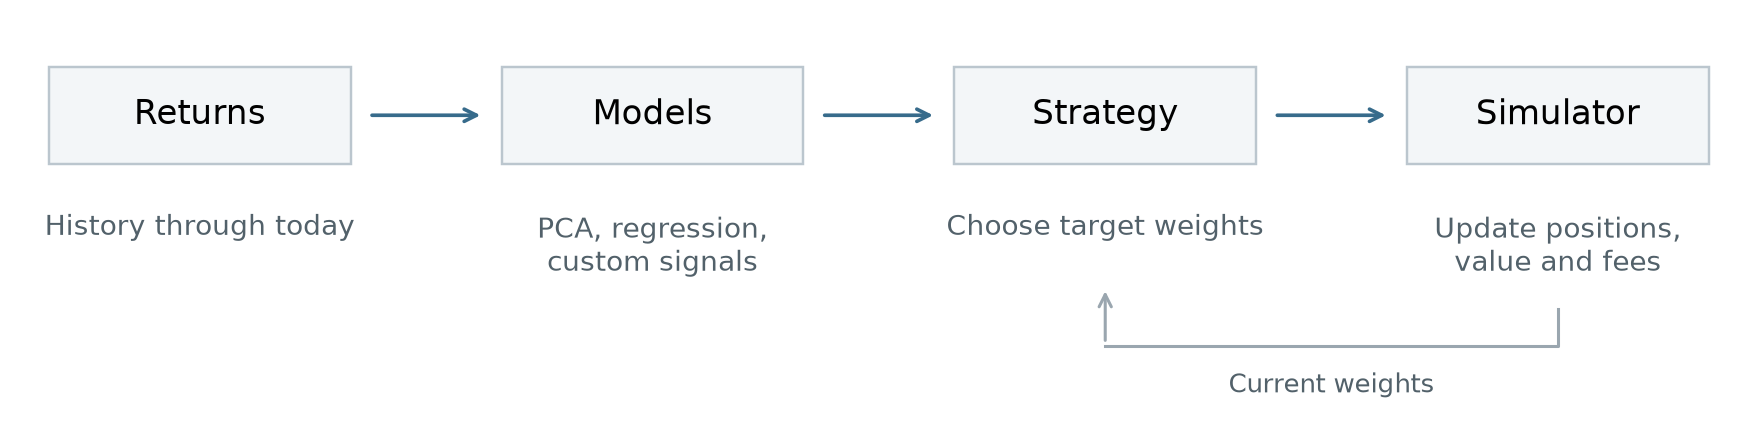
\includegraphics[width=\linewidth]{figures/framework_components.png}
    \caption{Daily data flow through the backtesting framework. Return
    history available through the current close enters the model sequence,
    which includes PCA, factor regression, and any custom signals.
    The strategy converts these outputs into target portfolio weights,
    while the simulator handles positions, returns, trades, and fees.
    The return arrow supplies the strategy with current weights after
    market movements, allowing it to calculate the next adjustment.
    The diagram shows one strategy, but several independent portfolios
    can use the same model outputs.}
    \label{fig:framework-components}
\end{figure}

\subsection{Rolling estimates}

Our PCA and factor models use rolling windows: fixed-length segments of
recent return history that advance as new observations arrive. Each model
has a configurable window length and refitting interval, which determine
how much history enters a fit and how often the estimate changes.
For example, a PCA model with a 500-day window and a five-day interval
fits on the latest 500 returns, reuses the estimate for four more days,
and then refits on the updated window. Because the factor regression has
its own window and interval, a strategy can estimate common factors from
a longer history while allowing stock exposures to respond more quickly
to recent observations.

At a PCA refit, we subtract each stock's mean and divide by its sample
standard deviation within that window, preventing highly volatile stocks
from dominating solely because of their larger return variation. After
retaining the leading \(K\) components, the regression converts them into
factor weights using the same volatility estimates and calculates factor
returns over its own window. Regressing each stock's returns on these
factors and an intercept then produces its estimated alpha and exposures.

To maintain a consistent factor definition within each regression, all
observations use the same active PCA weights. A new PCA estimate therefore
triggers a regression refit even before the regression's usual interval
elapses. Between refits, coefficients remain fixed while factor returns
and residuals update with each day's observations.

The same timing restriction applies to every stage of estimation,
including standardization, so future returns and volatility cannot enter
an earlier fit. Refitting also leaves earlier trading decisions unchanged.
Together, these conventions avoid look-ahead from model estimation,
although they do not eliminate the selection bias associated with
developing strategies through repeated experiments.

Custom signal models use the same daily flow, managing their own windows
and update schedules from the history of earlier outputs. When a model
learns from a five-day return, for example, that observation enters training
only after the full holding period ends. Strategies receive the updated
estimates through a common interface without changes to the simulation.

\begin{figure}[htbp]
    \centering
    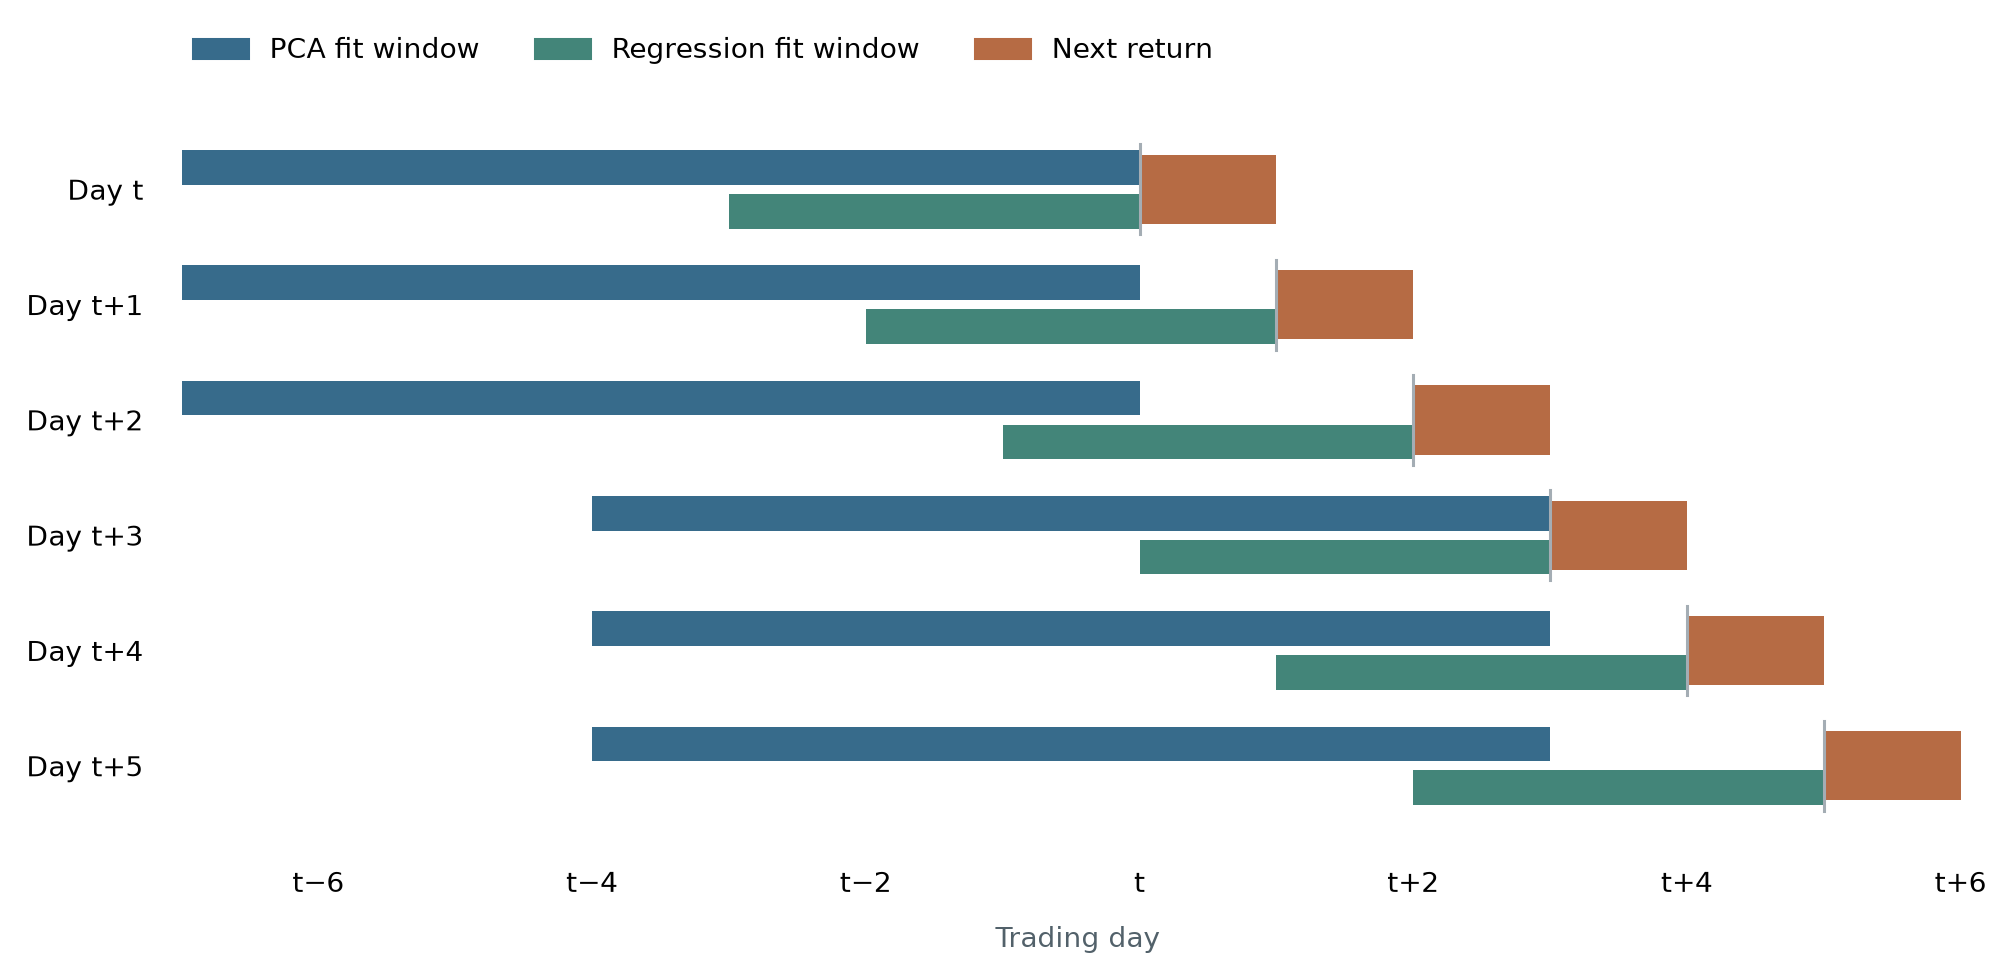
\includegraphics[width=\linewidth]{figures/framework_walkforward.png}
    \caption{Walk-forward estimation over six consecutive decision dates.
    Each row represents the portfolio decision at the indicated day's
    close, marked by the vertical gray line. Blue bars identify the
    observations used by the active PCA estimate, and green bars identify
    the regression window. In this example, PCA refits at \(t\) and
    \(t+3\), so its estimation window remains unchanged for three rows
    before advancing. The regression refits daily using the active PCA
    weights, including a new factor basis when PCA updates. Orange bars
    show the subsequent return interval earned by the chosen portfolio.
    Estimation periods lie entirely before or at the decision close,
    while portfolio returns occur afterward. Window lengths and the
    three-day PCA interval are illustrative rather than strategy defaults.}
    \label{fig:framework-walkforward}
\end{figure}

\subsection{Cool sidenote: PCA optimization}

Rolling PCA requires repeatedly fitting the model as the window advances,
which becomes slow when we test many parameter settings. Our basic
implementation computes all 1,201 eigenvalues and eigenvectors of the
stock covariance matrix, even when we use only five factors. We replace
this full decomposition with an iterative solver that computes only the
largest \(K\) eigenvalues and their eigenvectors. Comparing the methods
on the same return windows, we find that a 500-day fit with 1,201 stocks
and five factors takes about 264 ms with the basic method and 13.1 ms
with the optimized method, giving a median paired speedup of roughly
\(19\times\). The figures below compare runtime across different problem
sizes and show that the resulting eigenvalues and factor subspaces agree
closely. The gain is smaller for small stock universes, but it substantially
reduces the cost of repeated PCA fits on our full dataset.

\begin{figure}[htbp]
    \centering
    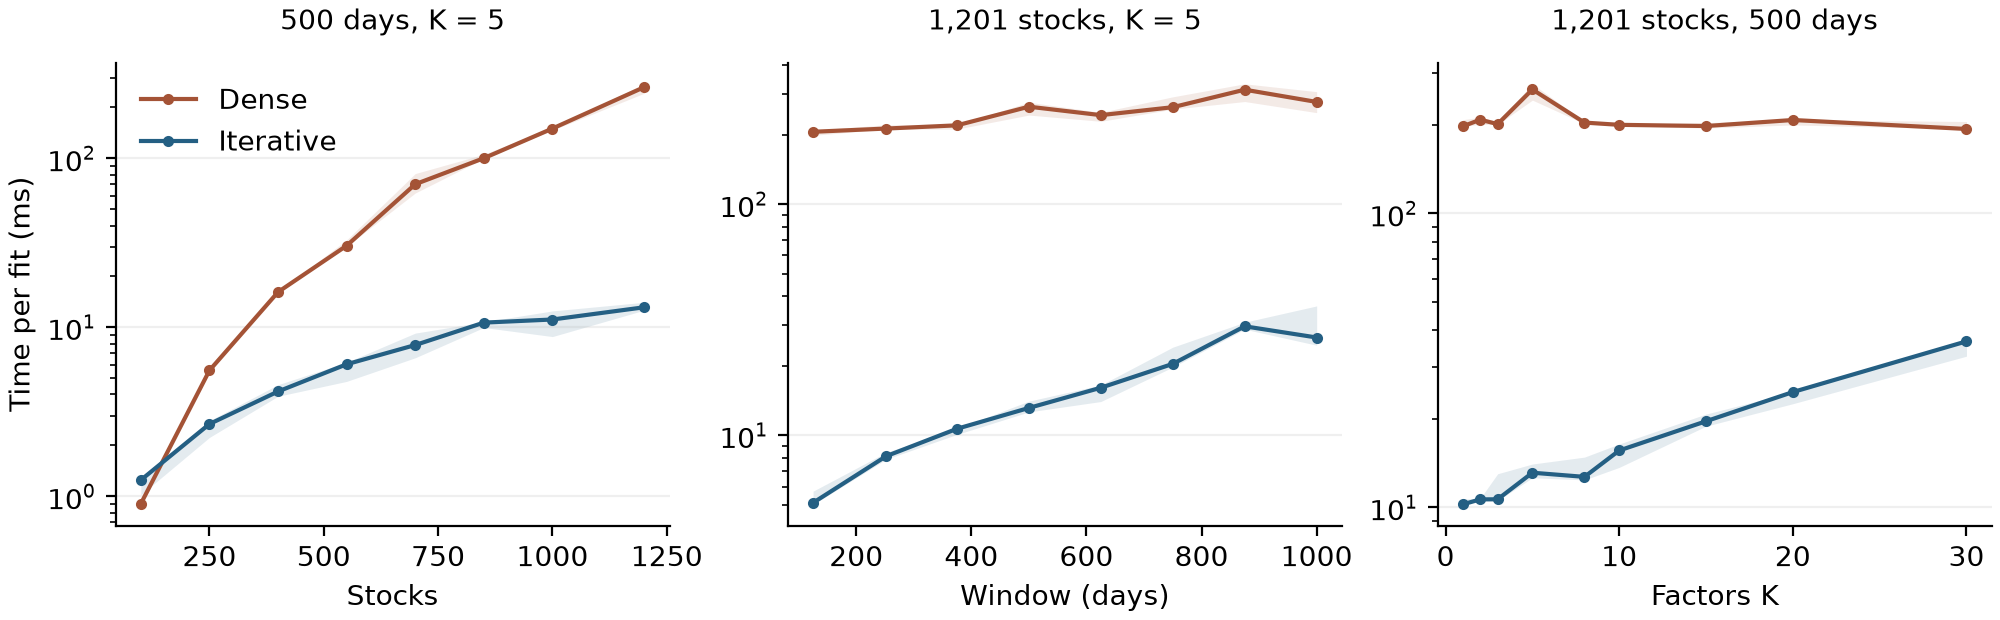
\includegraphics[width=\linewidth]{figures/pca_benchmark.png}
    \caption{PCA runtime as stock count, window length, and factor count
    vary, with other settings fixed as indicated above each panel.
    Points summarize the median of three window medians, each based on
    five runs. Shading spans the window medians rather than a confidence
    interval. Times include standardization and fitting, and the vertical
    axes are logarithmic. The iterative method's
    advantage grows with universe size but decreases as more factors
    are requested.}
    \label{fig:pca-benchmark}
\end{figure}

\begin{figure}[htbp]
    \centering
    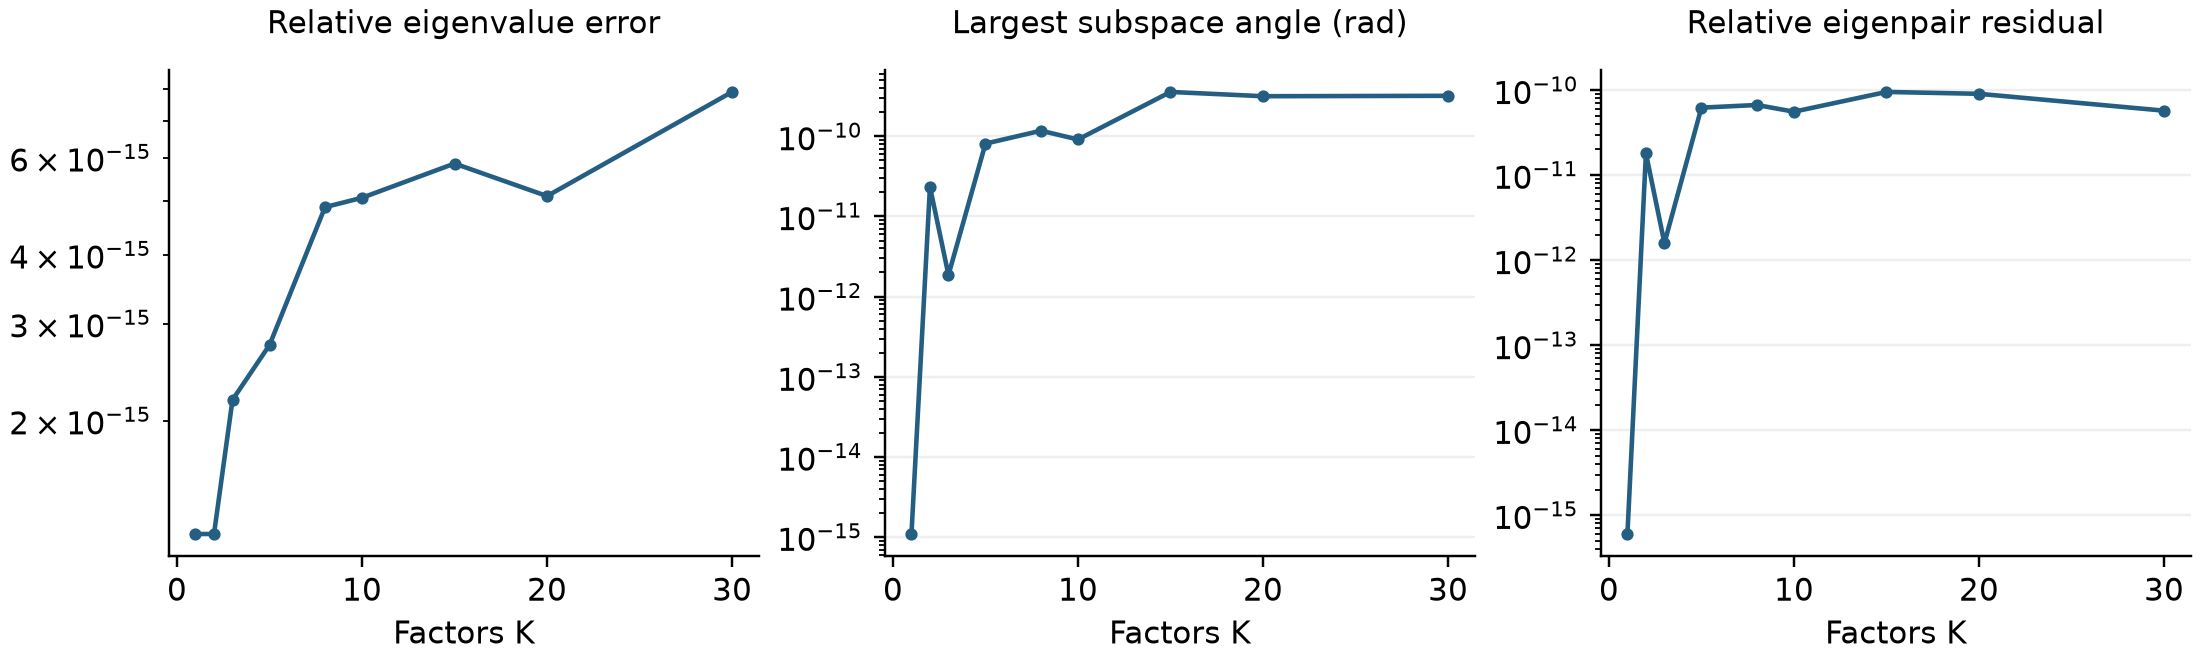
\includegraphics[width=\linewidth]{figures/pca_agreement.png}
    \caption{Numerical accuracy for 1,201 stocks and 500-day windows.
    The panels show relative eigenvalue differences, the largest angle
    between factor subspaces, and relative eigenpair residuals. Subspace
    angles account for arbitrary eigenvector signs, while residuals check
    the covariance eigenvalue equation directly. Each point is the worst
    value across three windows and five fits. Lower is better, and the
    logarithmic vertical axes have different scales. All checks pass
    the respective limits of \(10^{-8}\), \(10^{-6}\) radians, and
    \(10^{-8}\).}
    \label{fig:pca-agreement}
\end{figure}

\subsection{Execution and trading costs}

Our simulator applies daily returns to existing positions before executing
the next portfolio adjustment. Positions carried into day \(t\) therefore
earn that day's returns, while newly chosen weights \(w_{i,t}\) earn
returns on day \(t+1\):
\[
    r_{\mathrm{port},t+1}^{\mathrm{gross}}
    = \sum_i w_{i,t}r_{i,t+1}.
\]
Strategies hold cash until their required estimates are available, after
which we assume execution at the close used to calculate the signal.
This approximates observing prices immediately before the close and
submitting orders in time, but abstracts from processing delays and
differences between observed and executed prices. Introducing an additional
day of delay tests how strongly performance depends on immediate execution.

We calculate turnover from the weights after market movements to the new
targets, capturing the trades needed to restore an allocation even when
its target is unchanged. Positions held without adjustment incur no
rebalancing charge. The baseline deducts 5 basis points per dollar bought
or sold, including both entry and exit, while comparisons at higher fee
levels assess the sensitivity of net returns to execution costs.

\subsection{Strategy development and evaluation}

We divide evaluation into chronological training, validation, and final
holdout periods, using the training sample to develop signals and compare
candidate settings. Validation then assesses their performance on later
observations and informs the final selection. This chronological structure
preserves the order in which information becomes available, whereas a
random split would allow later market conditions to influence choices
evaluated on earlier observations.

Before the final holdout, we fix the trading rules, parameter settings,
cost assumptions, missing-data treatment, and performance measures, then
evaluate the holdout exactly once and retain the result regardless of
performance. This separates the final assessment from strategy selection.
Model estimates continue to update as observations arrive, but their
update rules remain fixed. A 500-day window, for example, continues to
advance without its length being reconsidered in response to holdout
results.

Each strategy section follows the same sequence so readers can compare
the evidence:
\begin{enumerate}
    \item \textbf{Strategy specification.} Explain the signal's motivation
    and conversion into weights, specifying estimation windows, refitting
    and trading intervals, and exposure limits.
    \item \textbf{Performance.} Report gross and net cumulative returns,
    annual results, drawdowns, and turnover to identify concentration in
    exceptional years and the contribution of trading costs.
    \item \textbf{Parameter sensitivity.} Vary nearby settings and factor
    count \(K\) over common dates after the longest warm-up. Compare
    full-sample and rolling estimates to assess how future information
    affects performance and the apparent preferred factor count.
    \item \textbf{Signal validation.} Compare subsequent returns across
    signal-strength groups and holding periods, accounting for dependence
    between overlapping returns when assessing uncertainty.
    \item \textbf{Implementation sensitivity.} Test higher fees, delayed
    execution, and exposure drift to identify dependence on low costs,
    immediate fills, or unintended risk.
    \item \textbf{Final holdout.} Report the fixed strategy's holdout result
    alongside training and validation performance, including deterioration.
\end{enumerate}

We report Sharpe ratios using daily returns, a zero risk-free-rate
convention, and annualization by \(\sqrt{252}\). For the assignment's
information ratio, we subtract fitted market exposure from portfolio
returns, divide their mean by their standard deviation, and apply the
same annualization. We state the benchmark and report market beta so
readers can see whether profits come with market exposure.

\subsection{Limitations}

Our tests address information timing, parameter sensitivity, and execution
assumptions, but the following biases and modeling limits remain relevant
when interpreting performance.

\begin{itemize}
    \item \textbf{Multiple-testing bias and validation overfitting.}
    Searching across signals and settings increases the chance of selecting
    a result that partly reflects luck. Repeated validation also makes
    those observations part of strategy selection, even when individual
    backtests use rolling estimates. Sensitivity checks and a final holdout
    strengthen the evidence without making the selected historical Sharpe
    ratio an unbiased estimate of future performance.

    \item \textbf{Survivorship and universe-selection bias.} The original
    panel contains long histories for 1,201 stocks over 2000--2023 and may
    underrepresent failed firms, delisted securities, and later entrants.
    Its selection procedure is unverified, so we cannot establish that
    the universe matches the securities available on each historical date.
    Rolling estimation restricts the information entering a fit but does
    not correct selection of the stocks themselves.

    \item \textbf{Execution and transaction-cost optimism.} Closing-price
    execution assumes negligible processing time and access to the observed
    price. Proportional fees omit market impact and stock-specific spreads,
    while the baseline also omits borrow costs and availability and assumes
    zero cash interest. These simplifications can overstate implementable
    returns. Higher-fee and delayed-execution tests assess sensitivity but
    do not establish achievable fills at a given portfolio size.

    \item \textbf{Regime dependence and limited external validity.} The
    final holdout covers one subsequent combination of volatility, liquidity,
    and investor behavior. Annual comparisons reveal concentration in
    particular episodes, but a successful holdout does not establish
    performance under different market conditions. Conclusions therefore
    apply to the observed periods without implying stable future returns.
\end{itemize}


\section{Trading strategies}
\label{sec:strategies}

We build three strategies on top of the PCA factor model. The first, a \emph{contrarian factor-neutral Treynor--Black portfolio}, trades directly on the estimated alphas $\alpha_i$. The second, \emph{PCA pairs trading}, uses the principal component loadings to find pairs of economically similar stocks and trades the convergence of their prices. The third, \emph{residual snapback}, buys stocks whose recent returns fell far short of what the factor model predicted, betting that the overreaction reverses.

The data are daily returns for $N = 1{,}201$ stocks from January 2000 to December 2023. All three strategies are simulated out-of-sample: every estimate is recomputed on a trailing window as the simulation moves forward. Trading begins in January 2002 once 500 days of history are available (April 2002 for residual snapback, which also needs a residual history; see Section~\ref{sec:snapback}).

\subsection{Rolling factor model}

\begin{itemize}
    \item \textbf{Principal components.} Every 5 trading days, we run PCA on the correlation matrix of the previous 500 days of returns. Standardizing returns first prevents high-volatility stocks from dominating the components. We keep the top $K = 5$ eigenvectors $v_1, \dots, v_5$.
    \item \textbf{Factor returns.} Each eigenvector defines an eigenportfolio with return $f^k_t = \sum_i \frac{v_k[i]}{\bar\sigma_i} r_{i,t}$.
    \item \textbf{Alphas and betas.} Each day, for each stock, we regress the previous 250 days of returns on the five factor returns,
    \[
        r_{i,t} = \alpha_i + \sum_{k=1}^{K} \beta_{k,i} f^k_t + \epsilon_{i,t},
    \]
    which gives the alpha $\alpha_i$, the factor betas $\beta_{k,i}$, and the residual variance $\sigma^2(\epsilon_i)$.
\end{itemize}

\subsection{Strategy 1: Contrarian factor-neutral Treynor--Black}

\paragraph{Scores.} Under the Treynor--Black model, the optimal active weight on a stock is proportional to its alpha divided by its idiosyncratic variance: a large alpha on a very noisy stock deserves less weight than a moderate alpha on a stable one. We use the negative of this ratio,
\[
    s_i = -\frac{\alpha_i}{\sigma^2(\epsilon_i)}.
\]
The sign is flipped because, out of sample, stocks with high estimated alpha go on to \emph{underperform} (Table~\ref{tab:development}). Past alpha in this universe reverses: it reflects temporary mispricing or estimation noise, not persistent outperformance. Section~\ref{sec:holdout} confirms that this reversal is already present using only 2002--2017 data. To keep a few extreme stocks from dominating, we convert the scores to cross-sectional z-scores and cap them at $\pm 3$.

\paragraph{Factor neutrality.} We project the scores onto the space orthogonal to a vector of ones and the $K$ beta vectors, so the portfolio satisfies
\[
    \sum_i w_i = 0 \quad \text{(dollar neutral)}, \qquad \sum_i w_i \beta_{k,i} = 0 \quad \text{for } k = 1, \dots, K \quad \text{(factor neutral)}.
\]
Because the first principal component is essentially the market, this also makes the strategy approximately market neutral.

\paragraph{Scaling and trading.} Weights are scaled so gross exposure is $\sum_i |w_i| = 1$ (50\% long, 50\% short), and the portfolio is rebalanced daily.

\begin{table}[!htbp]
\centering
\caption{Development of the strategy (out-of-sample, 2002--2023, 5bp fees unless stated).}
\label{tab:development}
\begin{adjustbox}{max width=\linewidth}
\begin{tabular}{lrrrr}
\toprule
Strategy & Sharpe & Sharpe (no fees) & Return & Market beta \\
\midrule
Long top 20\% $\alpha$, short bottom 20\% & $-1.31$ & $-0.98$ & $-6.1\%$ & $-0.07$ \\
Contrarian 20\% sort & 0.66 & 0.98 & 3.1\% & 0.07 \\
Contrarian 20\% sort, factor-hedged & 0.72 & 1.12 & 2.9\% & 0.04 \\
Contrarian Treynor--Black, not hedged & 0.76 & 1.18 & 2.4\% & 0.07 \\
\textbf{Contrarian Treynor--Black, factor-hedged} & \textbf{0.85} & \textbf{1.31} & 2.5\% & 0.04 \\
\bottomrule
\end{tabular}
\end{adjustbox}
\end{table}

Each design choice helps. Reversing the sign turns a losing strategy into a profitable one. Weighting by $\alpha_i / \sigma^2(\epsilon_i)$ improves on equal weights. The factor hedge leaves the return almost unchanged (2.5\% vs.\ 2.4\%) but lowers volatility from 3.2\% to 2.9\% and market beta from 0.07 to 0.04: it removes unrewarded factor risk without sacrificing alpha. Market beta is measured against an equal-weighted average of all stocks in the universe.

\begin{figure}[!htbp]
\centering
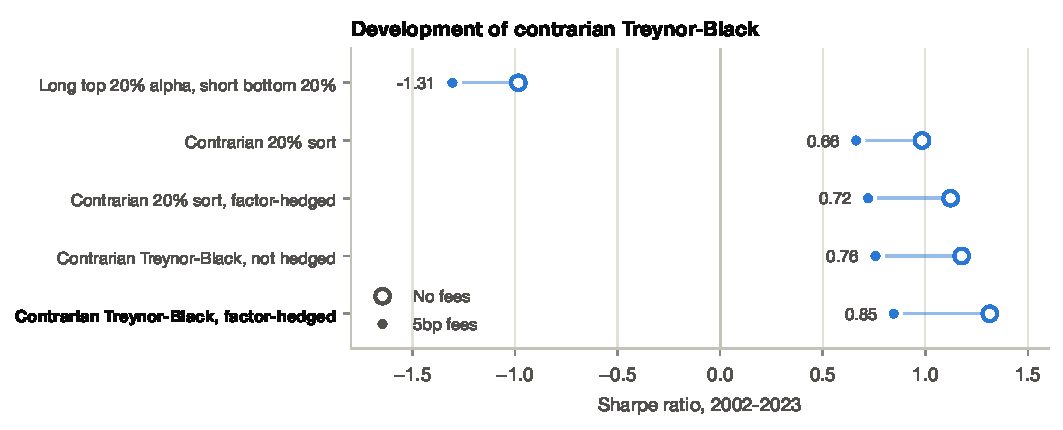
\includegraphics[width=0.85\textwidth]{figures/development_tb.pdf}
\caption{Development of the strategy (Table~\ref{tab:development}): Sharpe ratio of each step with 5bp fees (filled) and without fees (hollow).}
\label{fig:development-tb}
\end{figure}

\begin{figure}[!htbp]
\centering
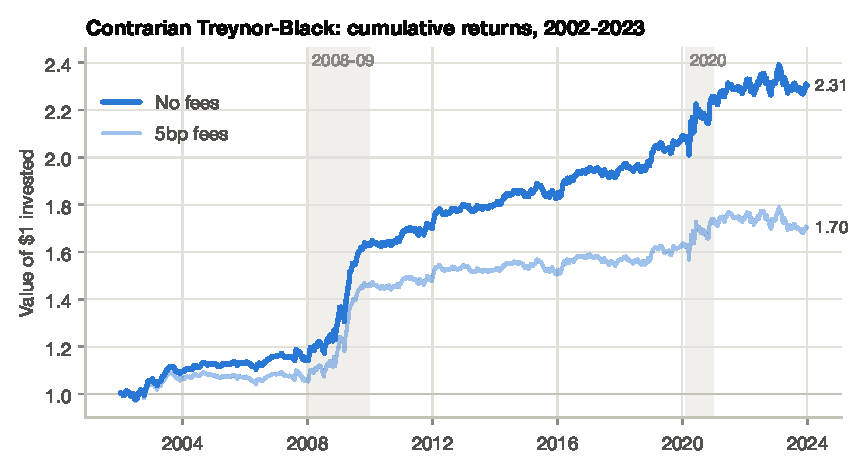
\includegraphics[width=0.88\linewidth]{figures/cumulative_returns_tb.pdf}
\caption{Growth of \$1 invested in Contrarian Treynor--Black, with and without 5bp transaction costs. Shaded regions mark the 2008--09 financial crisis and the 2020 COVID crash.}
\label{fig:cumulative-tb}
\end{figure}

\subsection{Strategy 2: PCA pairs trading}

\paragraph{Pair selection.} Every 21 trading days, we describe each stock by its loadings on the $K$ principal components, $\ell_i = (v_1[i]\sqrt{\lambda_1}, \dots, v_K[i]\sqrt{\lambda_K})$. We then greedily match the closest stocks in this space, keeping the 50 best non-overlapping pairs. Because the two stocks in a pair have nearly identical factor exposure, the spread between them is approximately factor neutral and driven mostly by stock-specific news.

\paragraph{Trading rule.} For each pair $(i, j)$, we track the log price ratio $\log(P_i / P_j)$ over the previous 60 days and compute its z-score $z$. When $z < -2$ we buy $i$ and short $j$; when $z > 2$ we do the reverse. We close the position once $|z| < 0.5$. Each pair is allocated a fixed $1/50$ of capital, so idle pairs hold cash.

Even though no industry data is used, the selected pairs are economically sensible: utilities (WEC/DUK, ATO/NI), natural gas producers (EQT/CNX), tower REITs (AMT/SBAC) and apartment REITs (EQR/MAA). The principal components recover industry structure from returns alone.

\begin{figure}[!htbp]
\centering
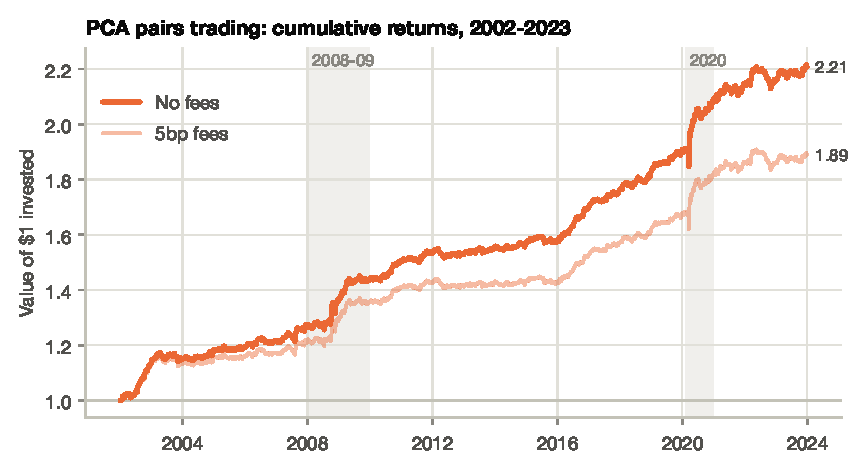
\includegraphics[width=0.88\linewidth]{figures/cumulative_returns_pairs.pdf}
\caption{Growth of \$1 invested in PCA pairs trading, with and without 5bp transaction costs. Shaded regions mark the 2008--09 financial crisis and the 2020 COVID crash.}
\label{fig:cumulative-pairs}
\end{figure}

\subsection{Strategy 3: Residual snapback}
\label{sec:snapback}

\paragraph{Idea.} The factor model splits each day's return into a part explained by the common factors and a stock-specific residual $\epsilon_{i,t}$. When a stock's residuals over the last few days are far more negative than usual, the stock has fallen much more than its factor exposures can explain. We treat this as an overreaction and buy the stock, expecting the gap to close. Treynor--Black trades on the \emph{level} of a stock's estimated alpha over the past year; snapback trades on a sharp, recent \emph{move} away from the model's prediction.

\paragraph{Lagged factor model.} Snapback uses its own version of the factor model. The PCA and the regression are fit on data through day $t-1$, and day $t$'s residual is then computed from those coefficients,
\[
    \epsilon_{i,t} = r_{i,t} - \alpha_i - \sum_{k=1}^{K} \beta_{k,i} f^k_t ,
\]
so the return being judged never enters the regression that judges it. The regression uses a 100-day window rather than Treynor--Black's 250 days. For Treynor--Black the alpha estimate \emph{is} the signal, so a long window reduces noise. For snapback the regression only provides a baseline for measuring surprises, and a shorter window lets that baseline follow recent changes in each stock's factor exposures, at the cost of noisier coefficient estimates.

\paragraph{Score.} A residual of $-5\%$ is extreme for a stable utility but routine for a volatile biotech, so we measure each residual against the stock's typical residual size. Let $\hat\sigma_{i,t}$ be the sample standard deviation of stock $i$'s residuals over the 60 days before the last three,
\[
    \hat\sigma_{i,t} = \sqrt{\frac{1}{59} \sum_{k=3}^{62} \left(\epsilon_{i,t-k} - \bar\epsilon_{i,t}\right)^2},
    \qquad
    \bar\epsilon_{i,t} = \frac{1}{60} \sum_{k=3}^{62} \epsilon_{i,t-k} .
\]
The score is the sum of the last three residuals in units of their expected spread,
\[
    s_{i,t} = \frac{\epsilon_{i,t-2} + \epsilon_{i,t-1} + \epsilon_{i,t}}{\sqrt{3}\, \hat\sigma_{i,t}} .
\]
The numerator is how far the stock has fallen short of (if negative) or run ahead of (if positive) the factor model over three days. If residuals have mean zero and are uncorrelated from day to day, the sum of three has variance $3\sigma_i^2$, so dividing by $\sqrt{3}\,\hat\sigma_{i,t}$ puts the score in standard-deviation units. Under these assumptions $s_{i,t}$ is roughly a standard normal draw, and $s_{i,t} \le -2$ marks an unusually large shortfall.

\paragraph{Checking the assumptions.} Both assumptions can be tested on the residuals themselves (Table~\ref{tab:residuals}). If the lagged model were biased, a negative residual sum could reflect the model's own error rather than a genuine shortfall. It is not biased: the mean residual across all stocks and days is $-0.003$bp per day ($t = -0.02$). The average across stocks of each stock's 60-day mean residual stays within a few basis points of zero throughout 2002--2023, including 2008--09 and 2020 (Figure~\ref{fig:residual-means}). Individual stocks' 60-day means spread about $\pm 25$bp per day (10th to 90th percentile), no wider than sampling noise alone would produce: with a typical daily residual volatility of 1.8\%, a 60-day mean has a standard error of about 23bp. One might expect the second assumption to fail in the other direction: if overreaction persists for several days, residuals would be positively correlated and $\sqrt{3}$ would understate the spread of their sum. In fact residuals are slightly \emph{negatively} correlated (median lag-1 autocorrelation $-0.03$), so a three-day sum varies about 5\% less than $\sqrt{3}$ assumes. The reversal the strategy bets on already begins within the three days. The $\sqrt{3}$ scaling is therefore close to right. Because it applies to every stock alike, a small error in it would mainly change how many stocks pass the $-2$ cutoff, not which stocks rank lowest. Across all stocks and days the scores have a standard deviation of 1.08, slightly above 1, because $\hat\sigma_{i,t}$ is estimated from only 60 days and residuals have fat tails.

\begin{table}[!htbp]
\centering
\caption{Residual diagnostics: lagged factor model, every stock and trading day, April 2002--2023.}
\label{tab:residuals}
\begin{adjustbox}{max width=\linewidth}
\begin{tabular}{lr}
\toprule
Measure & Value \\
\midrule
Mean residual (bp per day) & $-0.003$ \\
Newey--West $t$-statistic of the daily cross-sectional mean & $-0.02$ \\
Median daily residual volatility & 1.8\% \\
60-day mean residual, 10th / 90th percentile across stocks (bp per day) & $-25$ / 24 \\
Median autocorrelation of residuals, lag 1 / lag 2 & $-0.034$ / $-0.009$ \\
Median variance of 3-day sum / (3 $\times$ daily variance) & 0.95 \\
Standard deviation of the snapback score & 1.08 \\
\bottomrule
\end{tabular}
\end{adjustbox}
\end{table}

\begin{figure}[!htbp]
\centering
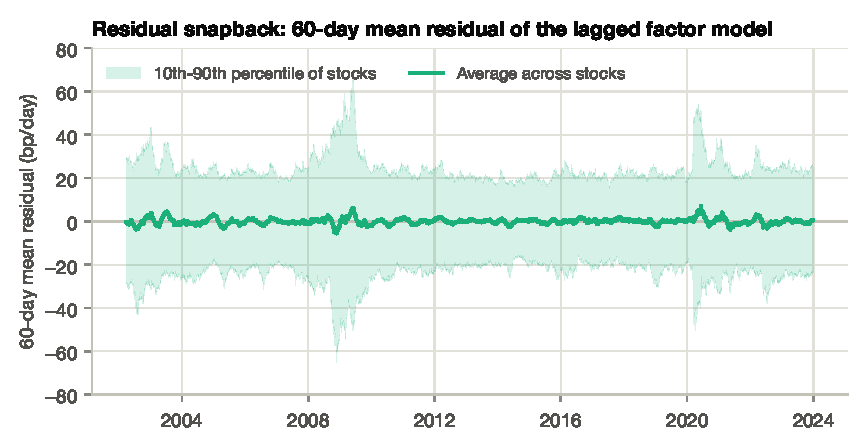
\includegraphics[width=0.88\linewidth]{figures/residual_means.pdf}
\caption{Residual diagnostics (Table~\ref{tab:residuals}): each stock's trailing 60-day mean residual from the lagged factor model. The line is the average across stocks, the band the 10th to 90th percentile.}
\label{fig:residual-means}
\end{figure}

\paragraph{Long-only version (default).} On the last trading day of each week we buy up to 20 stocks with the lowest scores, among those with $s_{i,t} \le -2$, in equal weights, and hold them until the next rebalance. If no stock qualifies, the portfolio holds cash. This default version is \emph{long only}, so it also carries the market.

\paragraph{Fully hedged version.} Even if the signal picks stocks that will beat the market, the long-only portfolio carries their factor exposures: an equal-weighted basket of stocks that have just fallen can load heavily on the market or on a sector-like component. The fully hedged version removes this exposure by trading the signal on both sides. On each rebalance date it takes up to 40 stocks with the lowest scores at or below $-2$ as long candidates and up to 40 stocks with the highest scores at or above $+2$ as short candidates, betting that stocks that ran unusually far ahead of the model will fall back. The starting weights $w^{(0)}_t$ put half the capital equally into the longs and half equally into the shorts: $w^{(0)}_{i,t} = 0.5 / n_L$ for each of the $n_L$ long candidates and $-0.5 / n_S$ for each of the $n_S$ short candidates. Let $B_t$ be the $K \times (n_L + n_S)$ matrix of the candidates' estimated betas, so $B_t w_t$ is the portfolio's factor exposure. We choose the weights closest to the starting weights that are factor neutral, have gross exposure 1 and keep the direction of each trade:
\[
\begin{aligned}
\min_{w_t} \quad & \tfrac{1}{2} \lVert w_t - w^{(0)}_t \rVert_2^2 \\
\text{subject to} \quad & B_t w_t = 0, \qquad \textstyle\sum_i |w_{i,t}| = 1, \\
& w_{i,t} \ge 0 \text{ for long candidates}, \qquad w_{i,t} \le 0 \text{ for short candidates}.
\end{aligned}
\]
Because each weight's sign is fixed, the gross-exposure constraint is linear, so this is a convex quadratic program; we solve it numerically (SLSQP). If either side has no candidates, or no weights satisfy the constraints, the hedged portfolio holds cash. The weights are not forced to be dollar neutral, but since the first factor is essentially the market, the portfolio is close to market neutral. An earlier version hedged only the long picks, projecting their equal weights onto the null space of their betas, which could short some of the 20 picks regardless of their scores. We keep it as a comparison row in Table~\ref{tab:snapback-variants}.

\paragraph{Fixed-weight hybrids.} The long-only version has the higher return; the hedged version has less risk. The hybrids construct both portfolios exactly as above and combine their weights,
\[
    w_t^{\text{hybrid}} = \lambda\, w_t^{\text{long only}} + (1 - \lambda)\, w_t^{\text{hedged}},
\]
for $\lambda = 0.7$, 0.5 and 0.3, to test whether a blend keeps some of the long-only upside while reducing exposure to common factor moves.

\paragraph{Volatility-weighted hybrid (dynamic).} A fixed $\lambda$ treats calm and turbulent markets alike, although factor risk matters most when markets are volatile. The dynamic version hedges more when volatility is high. Each day we compute the return of the equal-weighted universe and its sample standard deviation over the trailing 30 trading days. On each rebalance date we compare the current reading with all $n_t$ earlier readings and count the $k_t$ that are lower, with ties counting $\tfrac12$. The raw percentile $k_t / n_t$ is unstable when there are few earlier readings: the very first reading is both the highest and the lowest seen so far. We therefore add 126 pseudo-readings on each side (Laplace smoothing). The hedged weight is
\[
    \tilde p_t = \frac{k_t + 126}{n_t + 252}, \qquad
    w_t^{\text{dynamic}} = (1 - \tilde p_t)\, w_t^{\text{long only}} + \tilde p_t\, w_t^{\text{hedged}} .
\]
With no earlier readings the mix starts at 50/50, and the starting mix gets weight $252 / (n_t + 252)$, which shrinks as readings accumulate. For example, with 252 earlier readings a raw percentile of 90\% becomes a hedged weight of 70\%. When trading begins in 2002 about 470 readings are available, so the smoothing pulls the raw percentile about a third of the way towards 50\%; by 2023 the pull is about 4\% (Figure~\ref{fig:hedge-allocation}). An earlier version used the raw percentile and stayed fully long-only until 252 readings had accumulated; we keep it as a comparison row.

\begin{figure}[!htbp]
\centering
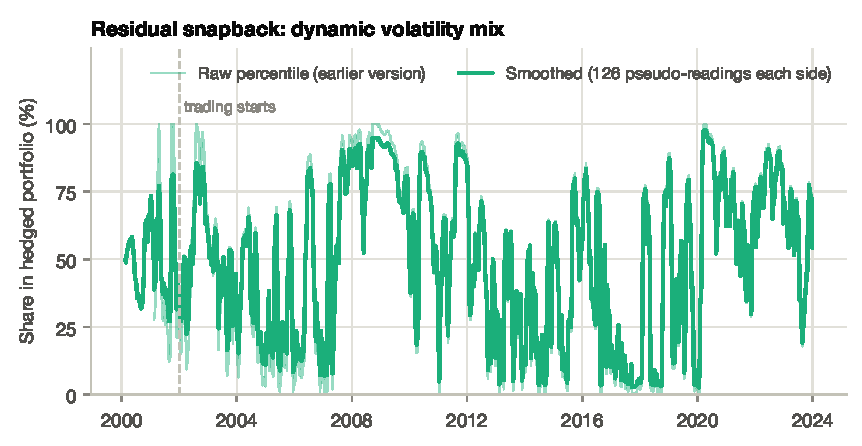
\includegraphics[width=0.88\linewidth]{figures/hedge_allocation.pdf}
\caption{Dynamic volatility mix: share of the portfolio in the fully hedged book at each weekly rebalance, using the smoothed percentile $\tilde p_t$ (dark) and the raw percentile of the earlier version (light).}
\label{fig:hedge-allocation}
\end{figure}

\paragraph{Cumulative residual score.} The snapback score only looks at the last three days. A stock that drifts below the factor model for weeks but then trades in line with it for three days has a snapback score near zero, even though its cumulative shortfall may be large. The cumulative score captures such drifts. We add each day's residual to a running total and compare today's level with its previous 60 levels:
\[
    X_{i,t} = X_{i,t-1} + \epsilon_{i,t}, \qquad
    z_{i,t} = \frac{X_{i,t} - \overline{X}^{(60)}_{i,t}}{s^{(60)}_{i,t}},
\]
where $\overline{X}^{(60)}_{i,t}$ and $s^{(60)}_{i,t}$ are the mean and sample standard deviation of $X_{i,t-60}, \dots, X_{i,t-1}$. The 60 days provide the reference level and scale, while the running total itself carries forward from day to day. A negative score means the running total is unusually far below its recent levels, and the hypothesis is again that unusually low levels rise and unusually high levels fall. The two scores are related but distinct: across all stocks and days their correlation is 0.47. We trade the cumulative score in two ways. First, with exactly the snapback rules above (weekly, long only or the 40/40 long-short book, cutoff $\pm 2$), using the same lagged factor model, so the only change is the score. Second, as a \emph{daily rank book}, the version developed on our group's residual-reversion branch: every day it buys the 20\% of stocks with the lowest scores and shorts the 20\% with the highest, with at most 2\% in any stock, then shrinks positions until the book is both dollar and factor neutral. This version uses an unlagged regression refit every five days, as on that branch.

\begin{table}[!htbp]
\centering
\caption{Residual snapback variants (out-of-sample, April 2002--2023).}
\label{tab:snapback-variants}
\begin{adjustbox}{max width=\linewidth}
\begin{tabular}{lrrrrrr}
\toprule
Variant & Sharpe & Sharpe (no fees) & Return & Volatility & Market beta & Max drawdown \\
\midrule
Equal-weight benchmark & 0.82 & 0.83 & 14.7\% & 18.8\% & 1.00 & $-53.0\%$ \\
\textbf{Long only (default)} & \textbf{0.82} & \textbf{1.03} & 19.1\% & 25.2\% & 1.08 & $-58.5\%$ \\
Stricter cutoff ($s_i \le -2.5$) & 0.67 & 0.86 & 15.3\% & 26.5\% & 1.08 & $-74.8\%$ \\
Hybrid, 70\% long only & 0.87 & 1.14 & 15.7\% & 18.8\% & 0.77 & $-45.0\%$ \\
Hybrid, 50\% long only & 0.91 & 1.26 & 13.1\% & 14.8\% & 0.57 & $-36.1\%$ \\
Hybrid, 30\% long only & 0.94 & 1.39 & 10.4\% & 11.3\% & 0.36 & $-30.3\%$ \\
Dynamic volatility mix & 0.96 & 1.39 & 11.3\% & 11.9\% & 0.31 & $-27.8\%$ \\
\textbf{Fully hedged (long-short)} & \textbf{0.76} & \textbf{1.38} & 6.1\% & 8.2\% & 0.06 & $-21.5\%$ \\
\midrule
\multicolumn{7}{l}{\emph{Earlier versions, for comparison}} \\
Projection hedge of the long picks & 0.83 & 1.23 & 10.2\% & 12.7\% & 0.12 & $-28.7\%$ \\
Dynamic mix, unsmoothed, projection hedge & 1.00 & 1.33 & 13.4\% & 13.5\% & 0.33 & $-32.8\%$ \\
\midrule
\multicolumn{7}{l}{\emph{Cumulative residual score}} \\
Long only (snapback rules) & 1.18 & 1.36 & 28.9\% & 23.9\% & 1.08 & $-53.2\%$ \\
Long-short (snapback rules) & 1.76 & 2.36 & 12.6\% & 6.9\% & 0.07 & $-10.4\%$ \\
Daily rank book & 3.01 & 4.41 & 9.5\% & 3.0\% & 0.05 & $-8.3\%$ \\
\bottomrule
\end{tabular}
\end{adjustbox}
\\[4pt]
\small 5bp fees unless stated. The benchmark holds every stock in equal weights, rebalanced weekly. Market beta is measured against the equal-weighted universe, as in Table~\ref{tab:development}.
\end{table}

The long-only default earns 19.1\% a year, but its Sharpe ratio after fees (0.82) only matches the equal-weight benchmark: most of its return and nearly all of its risk come from the market (beta 1.08). Regressing its daily returns on the market leaves an alpha of 3.6\% a year with 14.0\% residual volatility, an information ratio of 0.26. Hedging removes the market: the fully hedged long-short version has beta 0.06 and a market-adjusted alpha of 5.3\% a year with 8.2\% residual volatility (information ratio 0.65, close to Treynor--Black's 0.64 and below pairs trading's 1.05). Before fees its Sharpe ratio (1.38) is well above the long-only version's (1.03), but it trades as much as the long-only version on a smaller return, so after fees it falls to 0.76. Compared with the earlier projection hedge, the long-short book has lower risk (8.2\% vs.\ 12.7\% volatility, $-21.5\%$ vs.\ $-28.7\%$ drawdown) and a higher Sharpe ratio before fees (1.38 vs.\ 1.23), but a lower one after fees (0.76 vs.\ 0.83) and less alpha (5.3\% vs.\ 8.6\%). The hybrids and the dynamic mix have the highest Sharpe ratios after fees (0.87--0.96) because the long-only and hedged returns are imperfectly correlated. The mixes were chosen with the full sample in view; Section~\ref{sec:holdout} checks them out-of-sample. Because the long-only default is what the strategy was designed as, and the fully hedged version is the one comparable to the two market-neutral strategies, we test both throughout.

\begin{figure}[!htbp]
\centering
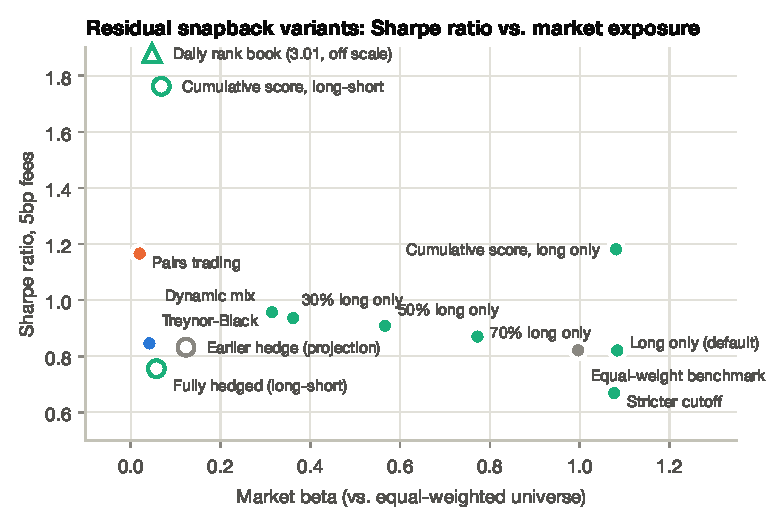
\includegraphics[width=0.75\textwidth]{figures/snapback_variants.pdf}
\caption{Residual snapback variants (Table~\ref{tab:snapback-variants}): Sharpe ratio with 5bp fees against market beta. Hollow markers are long-short books. The earlier projection hedge (gray) and the two market-neutral strategies are shown for reference. The daily rank book (Sharpe 3.01) is off scale.}
\label{fig:snapback-variants}
\end{figure}

Replacing the snapback score with the cumulative score improves both versions substantially, with nothing else changed: the long-only Sharpe ratio after fees rises from 0.82 to 1.18 and the long-short one from 0.76 to 1.76, above pairs trading's 1.17. The cumulative score also trades less (about 80--87 times a year rather than 100), so the long-short version breaks even at 20bp rather than 11bp. Both improvements hold in the 2018--2023 holdout (Table~\ref{tab:delay}). The daily rank book reaches a Sharpe ratio of 3.01 after fees (2.70 from 2004, reproducing the residual-reversion branch's result exactly).

Results this strong call for a check of how they would be executed. All our backtests trade at the closing price of the day the signal is computed. If part of a stock's residual on that day is noise in the closing price, such as a trade at the bid or the ask, the price partly reverts the next day. Trading at that same close then captures a reversal that could not be traded in practice. Table~\ref{tab:delay} repeats each version with every trade executed one day late. The daily rank book collapses from 3.01 to 0.25: almost all of its profit comes from the first day after the signal. The original snapback long-short book falls from 0.76 to 0.16. The weekly cumulative versions are the most robust, keeping a Sharpe ratio of 0.97 (long only) and 1.07 (long-short) when executed a day late. Their edge comes from a reversal that builds over weeks, not from the next day's bounce.

\begin{table}[!htbp]
\centering
\caption{Execution delay: Sharpe ratios (5bp fees) when trading at the signal's close and one day later.}
\label{tab:delay}
\begin{adjustbox}{max width=\linewidth}
\begin{tabular}{lrrrrr}
\toprule
& \multicolumn{2}{c}{Full period} & \multicolumn{2}{c}{At the signal's close} & \\
\cmidrule(lr){2-3} \cmidrule(lr){4-5}
Version & At close & One day late & 2002--2017 & 2018--2023 & Break-even fee \\
\midrule
Snapback score, long only & 0.82 & 0.65 & 0.91 & 0.62 & 25bp \\
Snapback score, long-short & 0.76 & 0.16 & 0.85 & 0.59 & 11bp \\
Cumulative score, long only & 1.18 & 0.97 & 1.27 & 0.97 & 37bp \\
Cumulative score, long-short & 1.76 & 1.07 & 2.03 & 1.26 & 20bp \\
Daily rank book & 3.01 & 0.25 & 3.93 & 1.43 & 16bp \\
\bottomrule
\end{tabular}
\end{adjustbox}
\\[4pt]
\small Each version from its first trade (April 2002). The selection and holdout columns therefore differ slightly from Table~\ref{tab:holdout}, which uses a common period from March 2004.
\end{table}

\begin{figure}[!htbp]
\centering
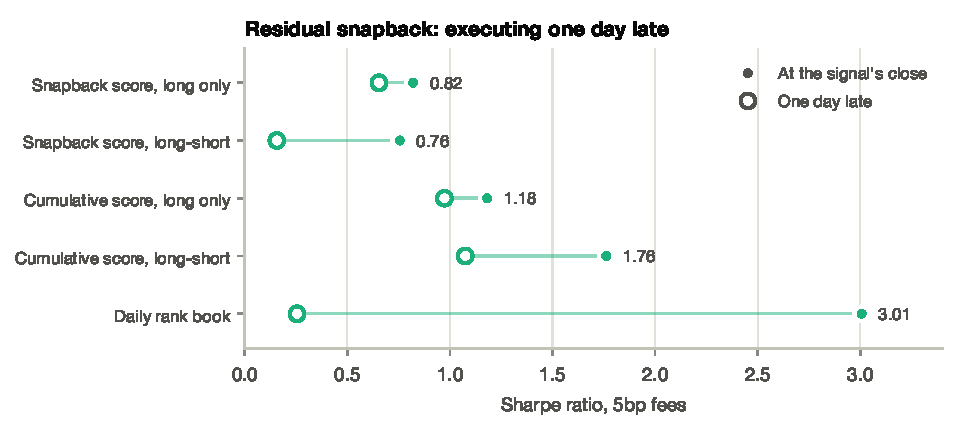
\includegraphics[width=0.85\textwidth]{figures/execution_delay.pdf}
\caption{Execution delay (Table~\ref{tab:delay}): Sharpe ratio with 5bp fees when trading at the signal's close (filled) and one day later (hollow).}
\label{fig:execution-delay}
\end{figure}

\begin{figure}[!htbp]
\centering
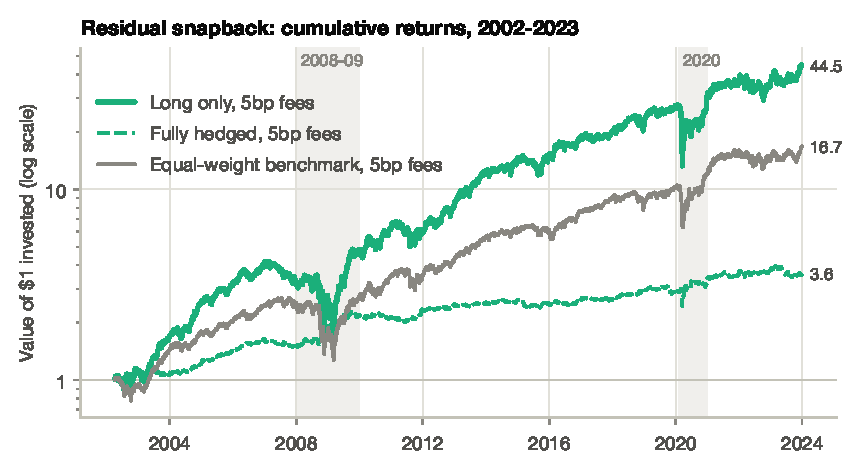
\includegraphics[width=0.88\linewidth]{figures/cumulative_returns_snap.pdf}
\caption{Growth of \$1 invested in residual snapback (long only and fully hedged) and the equal-weight benchmark, with 5bp transaction costs, on a log scale. Shaded regions mark the 2008--09 financial crisis and the 2020 COVID crash.}
\label{fig:cumulative-snap}
\end{figure}

\subsection{Backtest design}

\paragraph{Timing and look-ahead bias.} Weights chosen at the close of day $t$ use only returns up to and including day $t$, and they earn the returns of day $t+1$: $r_{\text{port},t+1} = \sum_i w_{i,t} r_{i,t+1}$. We verified this directly: re-running the backtest on data truncated at December 2011 leaves every earlier position unchanged, up to floating-point rounding of order $10^{-13}$. Residual snapback follows the same convention and additionally fits its factor model only through day $t-1$. Between weekly rebalances its positions drift with prices and are not traded.

\paragraph{Transaction costs.} The assignment defines returns without costs, so we report results both without fees and with a cost of 5 basis points per dollar traded.

\paragraph{Survivorship bias.} Every stock in the sample trades continuously from 2000 to 2023, so the universe consists of firms that survived the full period. Firms that failed or were acquired are missing. This likely flatters all three strategies, since buying a stock after a fall never ends in a delisting in this sample. Residual snapback is the most exposed, because buying stocks right after unusually large drops is its entire signal. This is a limitation of the data, not of the strategy code.

\section{Strategy testing}

We test all three strategies along six dimensions, reporting residual snapback in both its long-only and fully hedged forms. Unless stated otherwise, all results are out-of-sample, from January 2002 (April 2002 for snapback) to December 2023.

\subsection{Regime robustness}

\begin{table}[!htbp]
\centering
\caption{Annual returns and Sharpe ratios.}
\label{tab:yearly}
\begin{adjustbox}{max width=\linewidth}
\begin{tabular}{lrrrrrr}
\toprule
& \multicolumn{3}{c}{Contrarian Treynor--Black} & \multicolumn{3}{c}{PCA pairs trading} \\
\cmidrule(lr){2-4} \cmidrule(lr){5-7}
Year & Return & Return (5bp) & Sharpe & Return & Return (5bp) & Sharpe \\
\midrule
2002 & 5.6\% & 4.2\% & 1.93 & 13.8\% & 13.0\% & 3.52 \\
2003 & 3.6\% & 2.2\% & 1.64 & 0.9\% & 0.1\% & 0.33 \\
2004 & 2.6\% & 1.2\% & 1.51 & 2.6\% & 1.9\% & 1.02 \\
2005 & 0.7\% & $-0.7\%$ & 0.40 & 1.4\% & 0.7\% & 0.69 \\
2006 & 2.4\% & 1.1\% & 1.29 & 1.6\% & 0.8\% & 0.85 \\
2007 & $-1.1\%$ & $-2.4\%$ & $-0.38$ & 4.8\% & 4.0\% & 1.77 \\
2008 & 15.6\% & 13.7\% & 3.00 & 7.2\% & 6.2\% & 1.53 \\
2009 & 23.4\% & 21.5\% & 4.83 & 5.5\% & 4.8\% & 2.02 \\
2010 & 2.2\% & 0.8\% & 1.14 & 4.8\% & 4.1\% & 2.49 \\
2011 & 2.3\% & 0.8\% & 0.90 & 2.1\% & 1.3\% & 1.12 \\
2012 & 5.3\% & 3.9\% & 2.58 & $-0.6\%$ & $-1.2\%$ & $-0.42$ \\
2013 & 0.2\% & $-1.1\%$ & 0.14 & 1.8\% & 1.1\% & 0.94 \\
2014 & 2.7\% & 1.3\% & 1.62 & 1.1\% & 0.4\% & 0.79 \\
2015 & $-0.3\%$ & $-1.6\%$ & $-0.14$ & 0.1\% & $-0.6\%$ & 0.07 \\
2016 & 5.5\% & 4.1\% & 2.50 & 7.8\% & 7.0\% & 3.80 \\
2017 & 0.3\% & $-0.9\%$ & 0.14 & 3.9\% & 3.2\% & 2.28 \\
2018 & 1.7\% & 0.4\% & 0.70 & 3.6\% & 2.8\% & 2.06 \\
2019 & 5.1\% & 3.7\% & 2.46 & 4.5\% & 3.9\% & 2.71 \\
2020 & 8.1\% & 6.5\% & 1.26 & 9.5\% & 8.6\% & 1.91 \\
2021 & 1.6\% & 0.1\% & 0.61 & 2.7\% & 2.1\% & 1.14 \\
2022 & 1.6\% & 0.2\% & 0.44 & 0.7\% & $-0.1\%$ & 0.32 \\
2023 & $-0.8\%$ & $-2.1\%$ & $-0.22$ & 2.2\% & 1.6\% & 1.05 \\
\bottomrule
\end{tabular}
\end{adjustbox}
\\[4pt]
\small Returns and Sharpe ratios are without fees unless marked 5bp.
\end{table}

\begin{table}[!htbp]
\centering
\caption{Annual returns and Sharpe ratios: residual snapback.}
\label{tab:yearly-snap}
\begin{adjustbox}{max width=\linewidth}
\begin{tabular}{lrrrrrr}
\toprule
& \multicolumn{3}{c}{Long only} & \multicolumn{3}{c}{Fully hedged} \\
\cmidrule(lr){2-4} \cmidrule(lr){5-7}
Year & Return & Return (5bp) & Sharpe & Return & Return (5bp) & Sharpe \\
\midrule
2002 & 14.1\% & 9.9\% & 0.77 & 13.8\% & 9.7\% & 1.97 \\
2003 & 64.3\% & 56.1\% & 3.28 & 5.2\% & 0.0\% & 0.71 \\
2004 & 59.0\% & 50.9\% & 2.79 & 17.6\% & 11.7\% & 2.50 \\
2005 & 27.1\% & 20.7\% & 1.90 & 21.6\% & 15.5\% & 3.78 \\
2006 & 36.2\% & 29.4\% & 2.26 & 19.7\% & 13.7\% & 3.49 \\
2007 & $-14.9\%$ & $-19.1\%$ & $-0.79$ & $-1.4\%$ & $-6.3\%$ & $-0.18$ \\
2008 & $-20.7\%$ & $-24.6\%$ & $-0.18$ & 25.7\% & 19.6\% & 1.67 \\
2009 & 104.7\% & 94.3\% & 1.87 & 27.1\% & 20.9\% & 1.98 \\
2010 & 35.7\% & 28.9\% & 1.58 & 2.7\% & $-2.5\%$ & 0.44 \\
2011 & 1.5\% & $-3.5\%$ & 0.19 & 15.6\% & 9.8\% & 2.30 \\
2012 & 45.8\% & 38.5\% & 2.48 & 12.8\% & 7.2\% & 1.91 \\
2013 & 58.9\% & 51.0\% & 3.26 & 7.5\% & 2.2\% & 1.63 \\
2014 & 20.4\% & 14.3\% & 1.36 & 7.8\% & 2.4\% & 1.56 \\
2015 & 11.8\% & 6.1\% & 0.68 & 1.4\% & $-3.8\%$ & 0.26 \\
2016 & 28.5\% & 22.1\% & 1.60 & 8.9\% & 3.4\% & 1.44 \\
2017 & 13.8\% & 8.1\% & 1.16 & 5.9\% & 0.6\% & 1.05 \\
2018 & 13.2\% & 7.5\% & 0.85 & 17.7\% & 11.9\% & 3.20 \\
2019 & 34.3\% & 27.6\% & 2.06 & 4.3\% & $-0.9\%$ & 0.69 \\
2020 & 20.5\% & 14.5\% & 0.62 & 23.4\% & 18.0\% & 1.26 \\
2021 & 24.1\% & 17.9\% & 1.35 & 10.2\% & 4.7\% & 1.37 \\
2022 & 1.2\% & $-3.9\%$ & 0.18 & 9.4\% & 4.0\% & 1.10 \\
2023 & 31.9\% & 25.3\% & 1.49 & 1.3\% & $-3.7\%$ & 0.21 \\
\bottomrule
\end{tabular}
\end{adjustbox}
\\[4pt]
\small Returns and Sharpe ratios are without fees unless marked 5bp. 2002 starts in April.
\end{table}

\begin{table}[!htbp]
\centering
\caption{Concentration and stability of returns.}
\label{tab:regime}
\resizebox{\textwidth}{!}{%
\begin{adjustbox}{max width=\linewidth}
\begin{tabular}{lcccc}
\toprule
& & & \multicolumn{2}{c}{Residual snapback} \\
\cmidrule(lr){4-5}
Measure & Treynor--Black & Pairs trading & Long only & Fully hedged \\
\midrule
Years positive (no fees / 5bp) & 19 / 16 of 22 & 21 / 19 of 22 & 20 / 18 of 22 & 21 / 16 of 22 \\
Share of total profit from best year & 25\% (2009) & 16\% (2002) & 15\% (2009) & 10\% (2009) \\
Share of total profit from best two years & 43\% (2008--09) & 28\% (2002, 2020) & 25\% (2003, 2009) & 20\% (2008, 2009) \\
Sharpe, all years (no fees / 5bp) & 1.31 / 0.85 & 1.45 / 1.17 & 1.03 / 0.82 & 1.38 / 0.76 \\
Sharpe excluding best two years (no fees / 5bp) & 0.91 / 0.41 & 1.28 / 0.97 & 0.90 / 0.68 & 1.34 / 0.65 \\
Sharpe 2002--2012 / 2013--2023 (5bp) & 1.41 / 0.32 & 1.18 / 1.16 & 0.86 / 0.78 & 1.06 / 0.45 \\
Maximum drawdown (no fees / 5bp) & $-5.2\%$ / $-6.1\%$ & $-3.6\%$ / $-3.9\%$ & $-54.6\%$ / $-58.5\%$ & $-19.6\%$ / $-21.5\%$ \\
\bottomrule
\end{tabular}
\end{adjustbox}}
\end{table}

No single year carries any of the strategies, but they differ markedly (Figures~\ref{fig:cumulative-tb}--\ref{fig:annual-snap}). Treynor--Black earns its best returns in crises: in 2008 it gained 15.6\% while the market fell 27\%, followed by 23.4\% in 2009 and 8.1\% in 2020. These are periods of panic selling and overreaction, when betting on reversal should pay. However, 2008--09 account for 43\% of its total profit, and its Sharpe ratio after fees fell from 1.41 in 2002--2012 to 0.32 in 2013--2023. Pairs trading is far more stable: profitable in 21 of 22 years, no more than 28\% of profit from any two years, and an essentially identical Sharpe ratio in both halves of the sample.

Residual snapback has the least concentrated profits of the three: its best two years supply only about a quarter of the total. But it behaves very differently in crises. Long-only snapback lost 19.1\% in 2007 while the market rose 2\%, and 24.6\% in 2008, then gained 94\% in 2009. Buying the stocks that have just fallen hardest means catching falling knives in a sustained sell-off, and the long-only version carries the full market drawdown on top ($-58.5\%$ peak to trough, versus $-53\%$ for the benchmark). The fully hedged version behaves more like Treynor--Black: 2008 (25.7\%) and 2009 (27.1\%) are its two best years, and it cuts the maximum drawdown to $-21.5\%$. But its edge has faded: its Sharpe ratio after fees fell from 1.06 in 2002--2012 to 0.45 in 2013--2023, the second-largest decline after Treynor--Black's. Since 2013 it has lost money after fees in 2015, 2019 and 2023 and earned less than 2.5\% in 2013, 2014 and 2017.

\begin{figure}[!htbp]
\centering
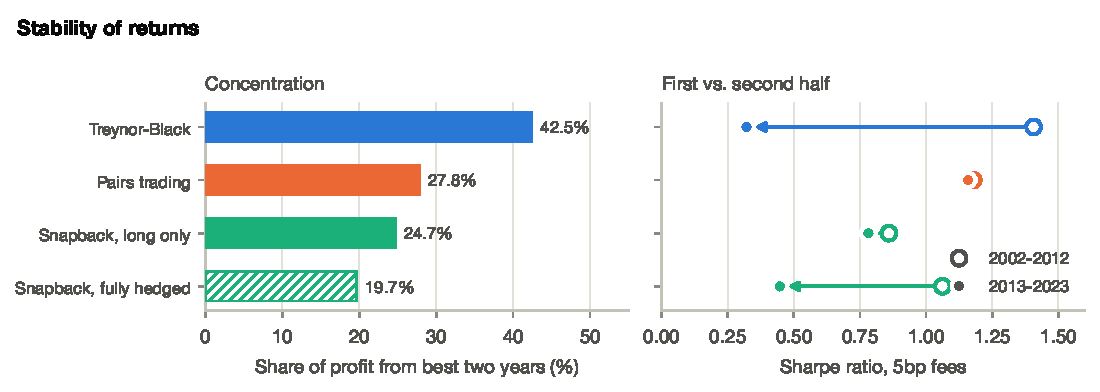
\includegraphics[width=\textwidth]{figures/regime_stability.pdf}
\caption{Concentration and stability of returns (Table~\ref{tab:regime}). Left: share of total profit (no fees) earned in each strategy's best two years. Right: Sharpe ratio with 5bp fees in 2002--2012 (hollow) and 2013--2023 (filled).}
\label{fig:regime-stability}
\end{figure}

\begin{figure}[!htbp]
\centering
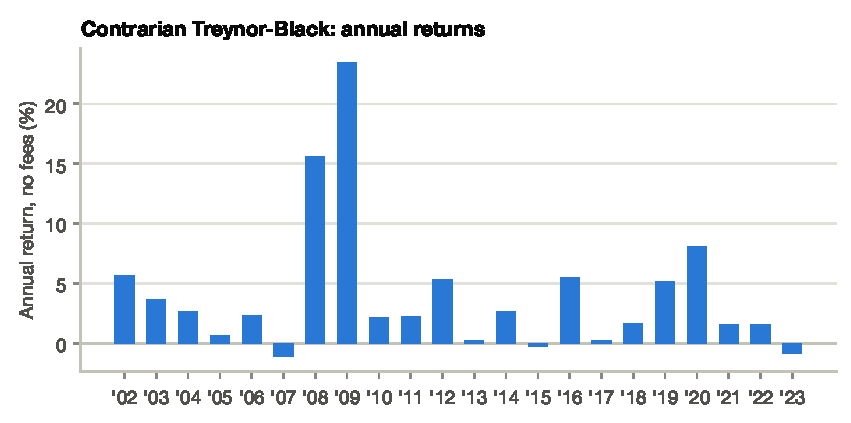
\includegraphics[width=0.88\linewidth]{figures/annual_returns_tb.pdf}
\caption{Annual returns of Contrarian Treynor--Black (no fees).}
\label{fig:annual-tb}
\end{figure}

\begin{figure}[!htbp]
\centering
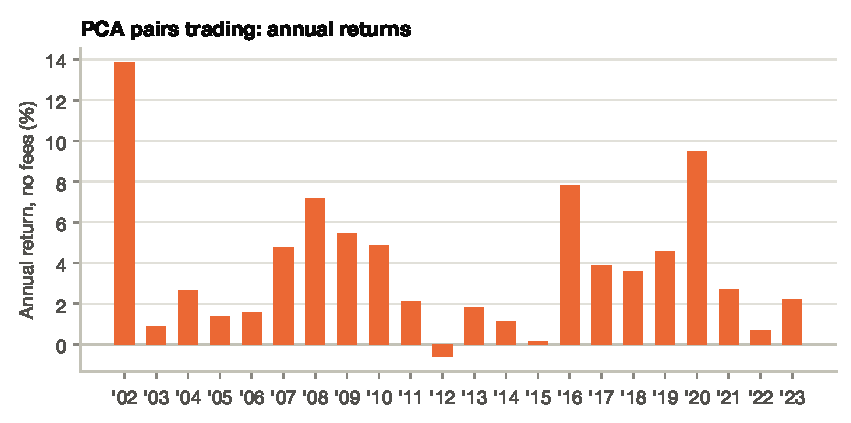
\includegraphics[width=0.88\linewidth]{figures/annual_returns_pairs.pdf}
\caption{Annual returns of PCA pairs trading (no fees).}
\label{fig:annual-pairs}
\end{figure}

\begin{figure}[!htbp]
\centering
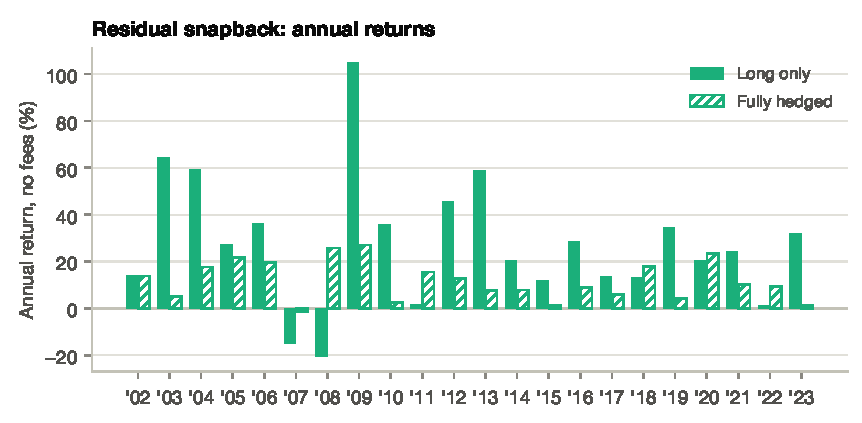
\includegraphics[width=0.88\linewidth]{figures/annual_returns_snap.pdf}
\caption{Annual returns of residual snapback, long only (solid) and fully hedged (hatched), no fees. 2002 starts in April.}
\label{fig:annual-snap}
\end{figure}

\subsection{Parameter sensitivity}

We vary one parameter at a time around the defaults. Because a 1000-day PCA window needs four years of history, all variants are compared over a common period: December 2003 onward for Treynor--Black and pairs trading, and March 2004 onward for residual snapback, whose lagged model and residual history need a few more months. The selection and holdout columns split this period into a selection period (through 2017) and a holdout period (2018--2023); see Section~\ref{sec:holdout}.

\begin{table}[!htbp]
\centering
\caption{Parameter sensitivity: contrarian Treynor--Black.}
\label{tab:sensitivity-tb}
\begin{adjustbox}{max width=\linewidth}
\begin{tabular}{llrrrrr}
\toprule
Parameter & Value & Sharpe & Sharpe (5bp) & Return (5bp) & Selection & Holdout \\
\midrule
Default & --- & 1.27 & 0.81 & 2.4\% & 1.08 & 0.40 \\
Alpha window (days) & 60 & 1.93 & 1.00 & 2.8\% & 1.13 & 0.83 \\
& 125 & 1.55 & 0.93 & 2.7\% & 1.13 & 0.64 \\
& 500 & 1.15 & 0.79 & 2.2\% & 0.88 & 0.64 \\
PCA window (days) & 250 & 1.25 & 0.78 & 2.3\% & 1.06 & 0.37 \\
& 1000 & 1.17 & 0.72 & 2.1\% & 0.96 & 0.36 \\
Score cap & 2 & 1.27 & 0.81 & 2.4\% & 1.10 & 0.39 \\
& 5 & 1.27 & 0.80 & 2.3\% & 1.06 & 0.41 \\
\bottomrule
\end{tabular}
\end{adjustbox}
\\[4pt]
\small Defaults: alpha window 250 days, PCA window 500 days, score cap 3. Selection and holdout columns include 5bp fees.
\end{table}

\begin{table}[!htbp]
\centering
\caption{Parameter sensitivity: PCA pairs trading.}
\label{tab:sensitivity-pairs}
\begin{adjustbox}{max width=\linewidth}
\begin{tabular}{llrrrrr}
\toprule
Parameter & Value & Sharpe & Sharpe (5bp) & Return (5bp) & Selection & Holdout \\
\midrule
Default & --- & 1.36 & 1.07 & 2.6\% & 1.04 & 1.15 \\
Entry threshold $|z|$ & 1.5 & 1.59 & 1.21 & 3.4\% & 1.20 & 1.25 \\
& 2.5 & 1.21 & 1.01 & 2.0\% & 0.92 & 1.19 \\
& 3 & 1.15 & 1.03 & 1.5\% & 0.99 & 1.14 \\
Exit threshold $|z|$ & 0 & 1.25 & 0.98 & 2.5\% & 0.97 & 1.02 \\
& 1 & 1.49 & 1.15 & 2.6\% & 1.05 & 1.37 \\
Spread window (days) & 20 & 1.93 & 1.43 & 3.4\% & 1.63 & 1.05 \\
& 40 & 1.59 & 1.25 & 3.1\% & 1.27 & 1.20 \\
& 120 & 1.29 & 1.08 & 2.6\% & 1.06 & 1.14 \\
Number of pairs & 20 & 0.68 & 0.48 & 1.7\% & 0.43 & 0.58 \\
& 100 & 1.73 & 1.38 & 2.7\% & 1.51 & 1.20 \\
Re-selection interval (days) & 5 & 1.54 & 1.14 & 2.5\% & 1.06 & 1.32 \\
& 63 & 1.42 & 1.19 & 3.1\% & 1.03 & 1.55 \\
PCA window (days) & 250 & 1.21 & 0.88 & 2.0\% & 0.76 & 1.13 \\
& 1000 & 1.54 & 1.28 & 3.3\% & 1.10 & 1.66 \\
Selection method & correlation & 1.89 & 1.35 & 1.6\% & 1.37 & 1.33 \\
\bottomrule
\end{tabular}
\end{adjustbox}
\\[4pt]
\small Defaults: entry 2, exit 0.5, spread window 60 days, 50 pairs, re-selection every 21 days, PCA window 500 days, selection by PCA loadings.
\end{table}

\begin{table}[!htbp]
\centering
\caption{Parameter sensitivity: residual snapback (Sharpe ratios, 5bp fees).}
\label{tab:sensitivity-snap}
\begin{adjustbox}{max width=\linewidth}
\begin{tabular}{llrrrrrr}
\toprule
& & \multicolumn{3}{c}{Long only} & \multicolumn{3}{c}{Fully hedged} \\
\cmidrule(lr){3-5} \cmidrule(lr){6-8}
Parameter & Value & Sharpe & Selection & Holdout & Sharpe & Selection & Holdout \\
\midrule
Default & --- & 0.76 & 0.83 & 0.62 & 0.76 & 0.87 & 0.59 \\
Signal days & 1 & 1.04 & 1.23 & 0.69 & 1.46 & 1.71 & 1.03 \\
& 5 & 0.84 & 0.92 & 0.68 & 0.80 & 0.52 & 1.40 \\
Volatility window (days) & 20 & 0.61 & 0.67 & 0.51 & 0.92 & 0.88 & 1.02 \\
& 120 & 0.78 & 0.81 & 0.72 & 0.93 & 1.03 & 0.78 \\
Score threshold & $-1.5$ & 0.83 & 0.91 & 0.67 & 0.91 & 1.15 & 0.68 \\
& $-2.5$ & 0.58 & 0.45 & 0.83 & 0.68 & 0.89 & 0.31 \\
& $-3$ & 0.48 & 0.33 & 0.77 & 0.36 & 0.44 & 0.20 \\
Maximum positions & 10 & 0.67 & 0.75 & 0.52 & 0.79 & 0.80 & 0.76 \\
& 50 & 0.81 & 0.87 & 0.68 & 0.83 & 0.87 & 0.77 \\
Rebalancing & daily & 0.84 & 0.96 & 0.60 & 0.89 & 0.96 & 0.83 \\
Regression window (days) & 60 & 0.75 & 0.83 & 0.59 & 0.56 & 0.64 & 0.43 \\
& 250 & 0.84 & 0.91 & 0.71 & 0.82 & 1.06 & 0.68 \\
PCA window (days) & 250 & 0.74 & 0.79 & 0.66 & 0.72 & 0.75 & 0.69 \\
& 1000 & 0.78 & 0.83 & 0.69 & 0.75 & 0.84 & 0.61 \\
Hedge mix & 70\% long only & 0.81 & 0.89 & 0.66 & & & \\
& 50\% long only & 0.86 & 0.95 & 0.69 & & & \\
& 30\% long only & 0.90 & 1.00 & 0.71 & & & \\
& dynamic & 0.88 & 1.06 & 0.51 & & & \\
\bottomrule
\end{tabular}
\end{adjustbox}
\\[4pt]
\small Defaults: 3 signal days, 60-day volatility window, threshold $-2$, up to 20 positions, weekly rebalancing, 100-day regression window, PCA window 500 days. The fully hedged version takes up to twice the maximum positions on each side (40 by default). Common period March 2004--2023.
\end{table}

Both strategies remain profitable after fees under every variant tested (Figures~\ref{fig:sensitivity-tb} and~\ref{fig:sensitivity-pairs}). Pairs trading is robust, with most Sharpe ratios between 0.9 and 1.4 after fees. The one weak variant is trading only 20 pairs (0.48), which concentrates risk in too few positions. Selecting pairs by return correlation gives a similar Sharpe ratio but a much lower return, partly because it selects two share classes of the same company (e.g.\ Brown-Forman, Berkshire Hathaway), which barely diverge. For Treynor--Black, shorter alpha windows perform better. This suggests that part of its edge comes from short-term reversal in the most recent returns entering the estimation window.

Residual snapback stays profitable after fees under every variant (Figure~\ref{fig:sensitivity-snap}). For the long-only version the model choices (regression window, PCA window) matter little; the hedged version is more sensitive to the regression window, falling to 0.56 with a 60-day window, presumably because noisier betas make the factor hedge less accurate. The signal design matters more. A one-day signal is the best variant in both versions (1.04 long only, 1.46 hedged), again pointing to very short-term reversal. Stricter thresholds lower the Sharpe ratio in both versions, plausibly because fewer stocks qualify and the portfolio is more concentrated, although for the long-only version they did better in the holdout. A 20-day volatility window gives a noisy estimate of $\hat\sigma_{i,t}$ and is the weakest choice for the long-only version. The hedged version's results move more between periods: its holdout Sharpe ratios range from 0.20 (threshold $-3$) to 1.40 (five signal days, which was among the worst variants in the selection period).

\begin{figure}[!htbp]
\centering
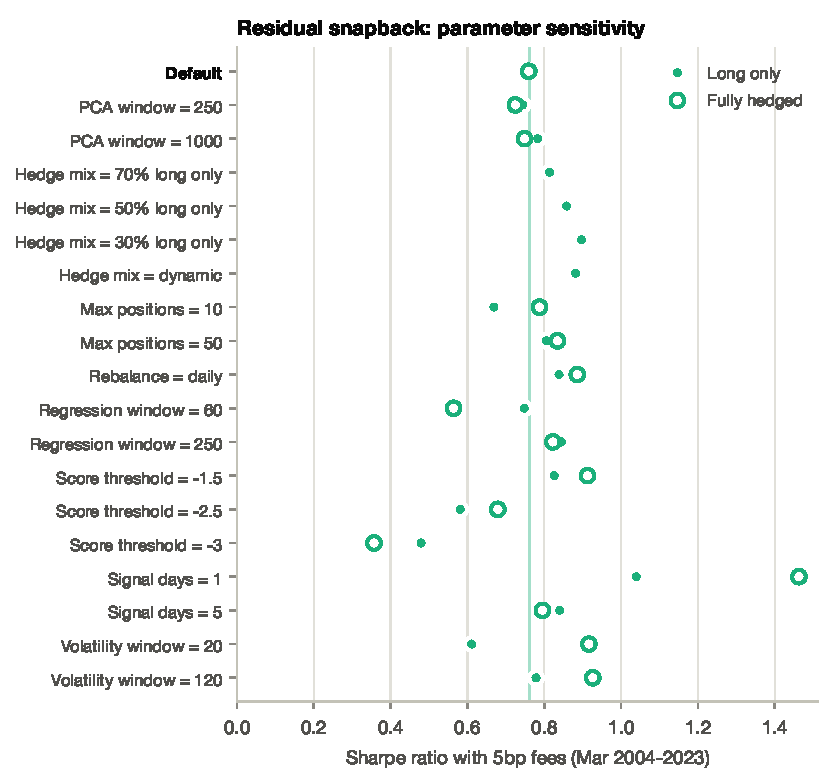
\includegraphics[width=0.7\textwidth]{figures/parameter_sensitivity_snap.pdf}
\caption{Sharpe ratio (5bp fees) of residual snapback for each parameter variant, long only (filled) and fully hedged (hollow). The vertical line marks the long-only default. Hedge mixes apply only to the long-only version.}
\label{fig:sensitivity-snap}
\end{figure}

\begin{figure}[!htbp]
\centering
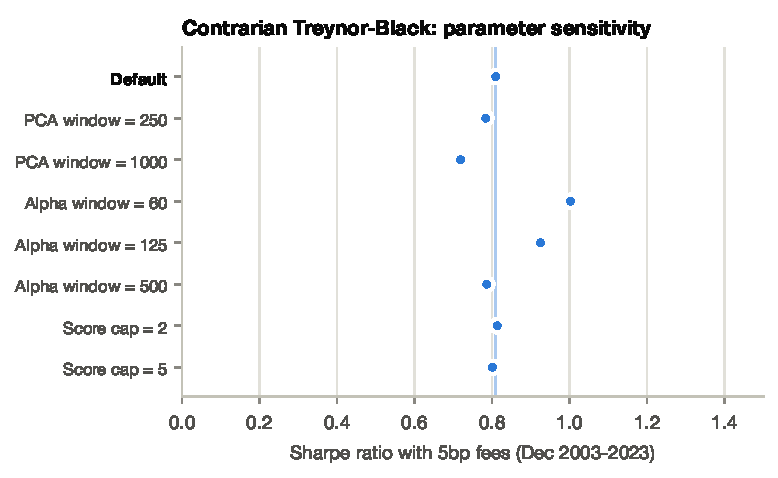
\includegraphics[width=0.7\textwidth]{figures/parameter_sensitivity_tb.pdf}
\caption{Sharpe ratio (5bp fees) of Contrarian Treynor--Black for each parameter variant. The vertical line marks the default settings.}
\label{fig:sensitivity-tb}
\end{figure}

\begin{figure}[!htbp]
\centering
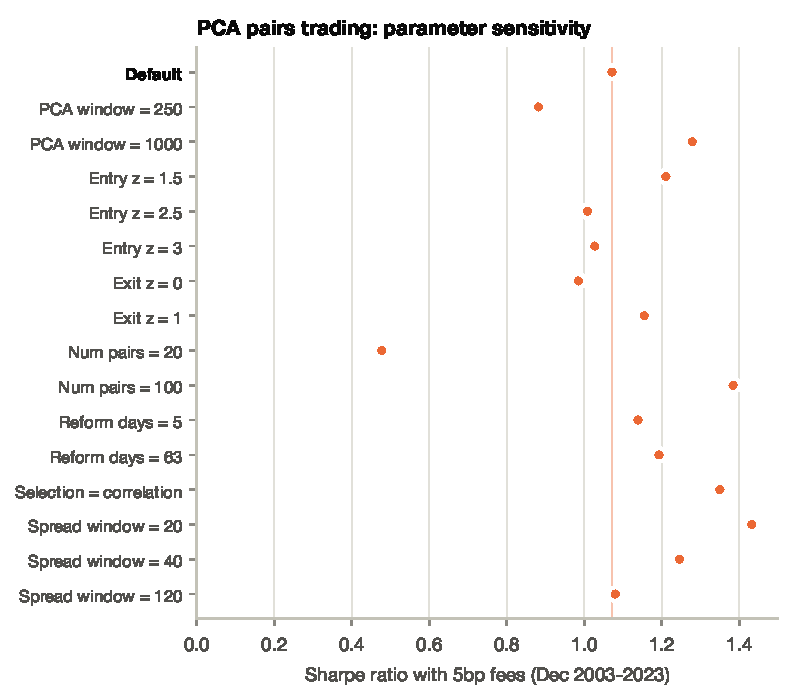
\includegraphics[width=0.7\textwidth]{figures/parameter_sensitivity_pairs.pdf}
\caption{Sharpe ratio (5bp fees) of PCA pairs trading for each parameter variant. The vertical line marks the default settings.}
\label{fig:sensitivity-pairs}
\end{figure}

\subsection{Trading costs}

\begin{table}[!htbp]
\centering
\caption{Turnover and the cost of trading.}
\label{tab:costs}
\begin{adjustbox}{max width=\linewidth}
\begin{tabular}{lcccc}
\toprule
& & & \multicolumn{2}{c}{Residual snapback} \\
\cmidrule(lr){4-5}
& Treynor--Black & Pairs trading & Long only & Fully hedged \\
\midrule
Daily turnover & 10.9\% & 5.6\% & 40.8\% & 40.3\% \\
Annual turnover & 28$\times$ & 14$\times$ & 103$\times$ & 102$\times$ \\
Gross return (annual mean) & 3.8\% & 3.6\% & 25.8\% & 11.3\% \\
Fee drag at 5bp (annual) & 1.4\% & 0.7\% & 5.2\% & 5.1\% \\
Share of edge lost at 5bp & 36\% & 20\% & 20\% & 45\% \\
Break-even fee & 14.0bp & 25.7bp & 25.0bp & 11.1bp \\
\midrule
Sharpe at 0bp & 1.31 & 1.45 & 1.03 & 1.38 \\
Sharpe at 2bp & 1.13 & 1.33 & 0.94 & 1.13 \\
Sharpe at 5bp & 0.85 & 1.17 & 0.82 & 0.76 \\
Sharpe at 10bp & 0.38 & 0.88 & 0.62 & 0.14 \\
Sharpe at 20bp & $-0.57$ & 0.32 & 0.21 & $-1.05$ \\
\bottomrule
\end{tabular}
\end{adjustbox}
\end{table}

Figures~\ref{fig:fees-tb}--\ref{fig:fees-snap} show how each strategy's Sharpe ratio falls with costs. Treynor--Black rebalances daily and turns over its portfolio 28 times a year, so costs take about a third of its edge, and it stops being profitable at around 14bp per trade. Pairs trading holds each position until the spread converges, halving turnover. It loses only a fifth of its edge to costs and survives fees up to about 26bp.

Residual snapback trades by far the most. Its holdings change almost completely every week, for a turnover of about 100 times a year, and fees cost 5\% a year at 5bp. The long-only version appears to survive this well (break-even 25bp), but only because its gross return includes the market, which costs nothing to trade. The fully hedged version, whose return is the strategy's own edge, loses 45\% of that edge at 5bp and breaks even at about 11bp, below Treynor--Black's 14bp. Trading costs are the main reason its Sharpe ratio of 1.38 before fees, close to pairs trading's 1.45, shrinks to 0.76.

\begin{figure}[!htbp]
\centering
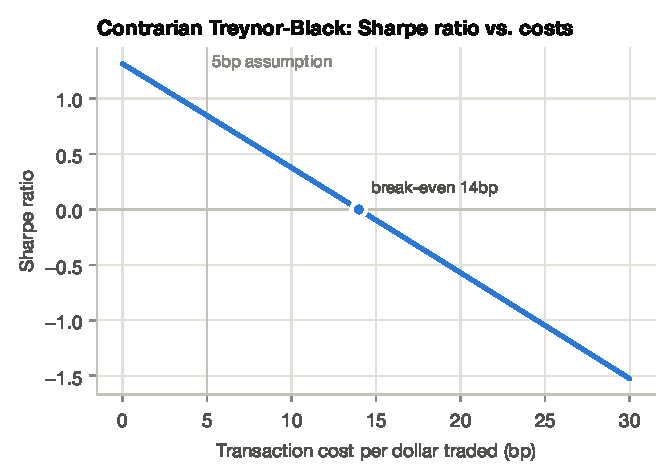
\includegraphics[width=0.65\textwidth]{figures/fee_sensitivity_tb.pdf}
\caption{Sharpe ratio of Contrarian Treynor--Black as a function of the transaction cost per dollar traded.}
\label{fig:fees-tb}
\end{figure}

\begin{figure}[!htbp]
\centering
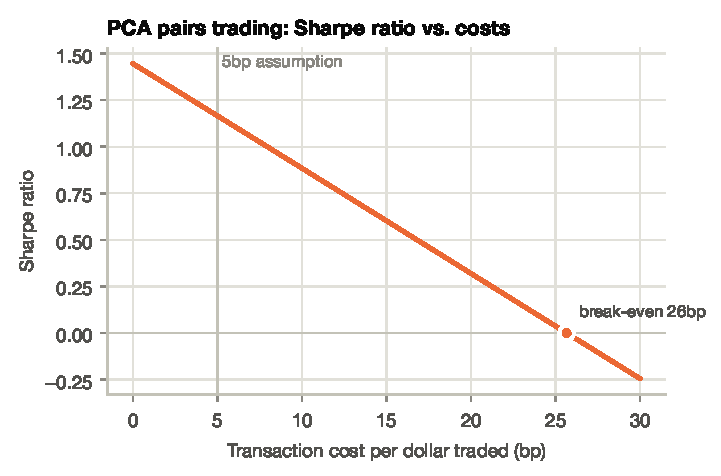
\includegraphics[width=0.65\textwidth]{figures/fee_sensitivity_pairs.pdf}
\caption{Sharpe ratio of PCA pairs trading as a function of the transaction cost per dollar traded.}
\label{fig:fees-pairs}
\end{figure}

\begin{figure}[!htbp]
\centering
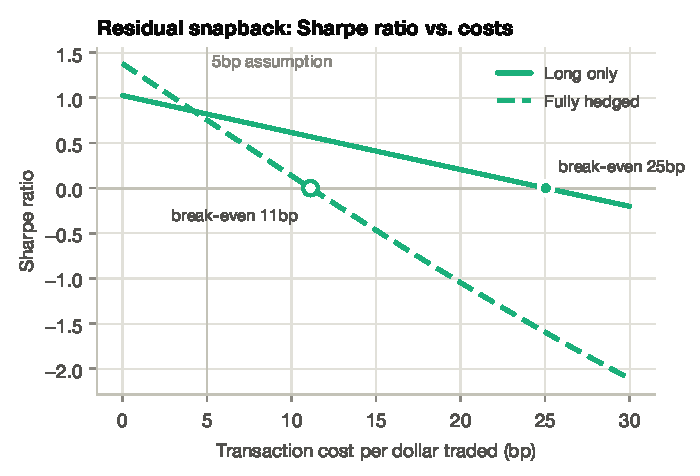
\includegraphics[width=0.65\textwidth]{figures/fee_sensitivity_snap.pdf}
\caption{Sharpe ratio of residual snapback, long only (solid) and fully hedged (dashed), as a function of the transaction cost per dollar traded.}
\label{fig:fees-snap}
\end{figure}

\subsection{Calibration}

To check that each signal predicts returns in the intended direction, we compare the signal on day $t$ with realized returns over the next $h$ days. For each day, we regress the realized return on the cross-sectionally standardized signal. Table~\ref{tab:calibration-slopes} reports the average slope with Newey--West $t$-statistics to account for overlapping horizons.

\begin{table}[!htbp]
\centering
\caption{Treynor--Black: mean excess return by signal decile (bp).}
\label{tab:calibration-tb}
\begin{adjustbox}{max width=\linewidth}
\begin{tabular}{lrrrrrrrrrr}
\toprule
Horizon & D1 & D2 & D3 & D4 & D5 & D6 & D7 & D8 & D9 & D10 \\
\midrule
1 day & $-3.0$ & $-2.0$ & $-1.3$ & $-1.0$ & 0.6 & 2.1 & 1.8 & 1.6 & 1.0 & 0.1 \\
5 days & $-10.7$ & $-6.6$ & $-1.7$ & $-1.0$ & 3.1 & 6.2 & 3.6 & 3.6 & 2.9 & 0.7 \\
20 days & $-34.4$ & $-17.4$ & $-0.5$ & 2.1 & 14.2 & 22.1 & 10.0 & 6.9 & 3.4 & $-6.1$ \\
\bottomrule
\end{tabular}
\end{adjustbox}
\\[4pt]
\small D1 is the decile the strategy shorts most (highest alpha), D10 the decile it buys most. Excess return is relative to the cross-sectional average.
\end{table}

\begin{table}[!htbp]
\centering
\caption{Pairs trading: mean change in the pair's log price ratio by spread z-score (bp).}
\label{tab:calibration-pairs}
\begin{adjustbox}{max width=\linewidth}
\begin{tabular}{lrrrr}
\toprule
Spread z-score & Next 1 day & Next 5 days & Next 20 days & Observations \\
\midrule
$z < -3$ & 48.4 & 108.4 & 157.9 & 2,251 \\
$-3$ to $-2$ & 17.7 & 20.8 & 43.9 & 16,811 \\
$-2$ to $-1$ & 7.0 & 13.5 & 8.3 & 56,696 \\
$-1$ to $0$ & 3.0 & 5.0 & $-0.8$ & 64,245 \\
$0$ to $1$ & $-3.5$ & $-6.3$ & $-31.8$ & 64,170 \\
$1$ to $2$ & $-7.2$ & $-14.3$ & $-53.1$ & 55,074 \\
$2$ to $3$ & $-18.3$ & $-46.2$ & $-101.7$ & 15,567 \\
$z > 3$ & $-59.7$ & $-143.8$ & $-267.5$ & 2,036 \\
\bottomrule
\end{tabular}
\end{adjustbox}
\end{table}

\begin{table}[!htbp]
\centering
\caption{Residual snapback: mean excess return by snapback score (bp).}
\label{tab:calibration-snap}
\begin{adjustbox}{max width=\linewidth}
\begin{tabular}{lrrrr}
\toprule
Snapback score $s_i$ & Next 1 day & Next 5 days & Next 20 days & Observations \\
\midrule
$s < -3$ & 13.1 & 46.6 & 67.1 & 52,973 \\
$-3$ to $-2$ & 10.8 & 25.8 & 40.4 & 118,870 \\
$-2$ to $-1$ & 9.7 & 17.4 & 24.5 & 653,346 \\
$-1$ to $0$ & 3.6 & 5.9 & 9.1 & 2,514,925 \\
$0$ to $1$ & $-4.2$ & $-6.8$ & $-9.5$ & 2,393,685 \\
$1$ to $2$ & $-7.7$ & $-15.2$ & $-27.0$ & 648,547 \\
$2$ to $3$ & $-9.3$ & $-22.9$ & $-34.4$ & 132,428 \\
$s > 3$ & $-18.3$ & $-42.8$ & $-39.4$ & 59,500 \\
\bottomrule
\end{tabular}
\end{adjustbox}
\\[4pt]
\small Every stock on every trading day, not only the stocks and weeks the strategy trades. Excess return is relative to the cross-sectional average. The strategy buys at $s \le -2$.
\end{table}

\begin{table}[!htbp]
\centering
\caption{Cumulative residual score: mean excess return by score (bp).}
\label{tab:calibration-cumulative}
\begin{adjustbox}{max width=\linewidth}
\begin{tabular}{lrrrr}
\toprule
Cumulative score $z_i$ & Next 1 day & Next 5 days & Next 20 days & Observations \\
\midrule
$z < -3$ & 19.8 & 60.5 & 86.3 & 83,025 \\
$-3$ to $-2$ & 8.8 & 18.7 & 32.2 & 408,691 \\
$-2$ to $-1$ & 3.9 & 8.5 & 17.8 & 1,282,369 \\
$-1$ to $0$ & 0.8 & 1.7 & 4.7 & 1,522,584 \\
$0$ to $1$ & $-0.7$ & $-2.2$ & $-3.6$ & 1,536,338 \\
$1$ to $2$ & $-4.2$ & $-8.9$ & $-19.7$ & 1,262,177 \\
$2$ to $3$ & $-8.5$ & $-19.6$ & $-38.0$ & 397,668 \\
$z > 3$ & $-19.4$ & $-45.7$ & $-56.9$ & 83,824 \\
\bottomrule
\end{tabular}
\end{adjustbox}
\\[4pt]
\small Same stocks, days and target as Table~\ref{tab:calibration-snap}, using the lagged factor model's residuals. Observations are for the next-day horizon.
\end{table}

\begin{table}[!htbp]
\centering
\caption{Return per one standard deviation of signal.}
\label{tab:calibration-slopes}
\resizebox{\textwidth}{!}{%
\begin{adjustbox}{max width=\linewidth}
\begin{tabular}{lrrrrrrrr}
\toprule
& \multicolumn{2}{c}{Treynor--Black} & \multicolumn{2}{c}{Pairs trading} & \multicolumn{2}{c}{Snapback score} & \multicolumn{2}{c}{Cumulative score} \\
\cmidrule(lr){2-3} \cmidrule(lr){4-5} \cmidrule(lr){6-7} \cmidrule(lr){8-9}
Horizon & Slope & $t$-stat & Slope & $t$-stat & Slope & $t$-stat & Slope & $t$-stat \\
\midrule
1 day & 1.1bp & 5.2 & 9.6bp & 13.3 & 6.0bp & 21.6 & 5.0bp & 18.1 \\
5 days & 3.4bp & 3.4 & 19.3bp & 7.3 & 11.4bp & 13.3 & 11.1bp & 10.9 \\
20 days & 7.7bp & 1.8 & 39.0bp & 4.7 & 17.1bp & 10.7 & 20.6bp & 7.4 \\
\bottomrule
\end{tabular}
\end{adjustbox}}
\\[4pt]
\small The pairs slope is per pair spread; the Treynor--Black and snapback slopes are per stock.
\end{table}

The pairs signal is very well calibrated (Figures~\ref{fig:calibration-tb} and~\ref{fig:calibration-pairs}). Future spread returns fall steadily with the z-score in every bucket and at every horizon, and the relationship is highly significant ($t = 13.3$ at one day). The Treynor--Black signal is significant at short horizons ($t = 5.2$) but only partly monotonic. Its predictive power is concentrated in the stocks it shorts: the highest-alpha decile underperforms strongly and persistently. The lowest-alpha stocks it buys most do not outperform, and at 20 days they underperform. In other words, high past alpha reverses, but very low past alpha does not. The edge also fades with horizon, consistent with the strategy's need for daily rebalancing.

The snapback score is as well calibrated as the pairs signal and the most statistically significant of the three (Figure~\ref{fig:calibration-snap}). Future excess returns fall monotonically across all eight score buckets at every horizon, and the slope has the highest $t$-statistic of any signal (21.6 at one day, still 10.7 at 20 days), helped by the much larger number of observations. Stocks in the buy zone ($s \le -2$) beat the cross-section by 26--47bp over the following week. The relationship is symmetric: stocks with unusually \emph{positive} residuals underperform just as reliably, which is what the fully hedged version's short leg exploits. Because the signal is so well calibrated, the strategy's modest Sharpe ratio comes from how the signal is traded (the market exposure of the long-only version and the heavy turnover), not from the signal itself.

The cumulative score is also monotonic in every bucket at every horizon (Table~\ref{tab:calibration-cumulative}). Its slope is slightly smaller than the snapback score's at one day (5.0bp vs.\ 6.0bp) but larger at 20 days (20.6bp vs.\ 17.1bp), and its most extreme buckets have larger returns ($+60$bp over five days for $z < -3$, against $+47$bp for the snapback score). This fits the execution-delay results: the cumulative score's predictive power lasts longer, so less of it is lost when trading weekly or a day late.

\begin{figure}[!htbp]
\centering
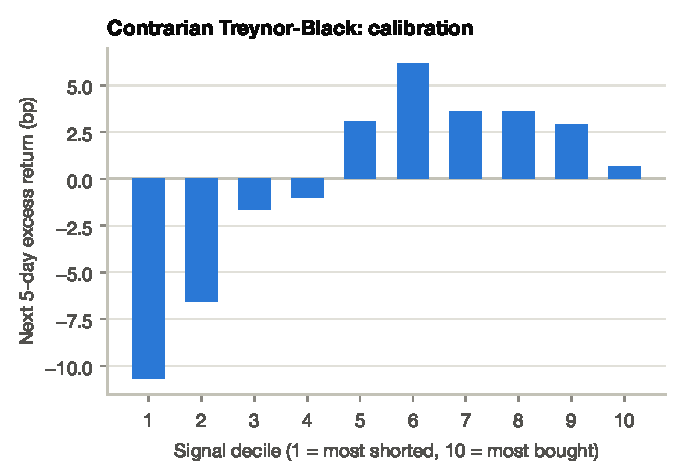
\includegraphics[width=0.65\textwidth]{figures/calibration_tb.pdf}
\caption{Calibration of Contrarian Treynor--Black: next 5-day excess return by signal decile.}
\label{fig:calibration-tb}
\end{figure}

\begin{figure}[!htbp]
\centering
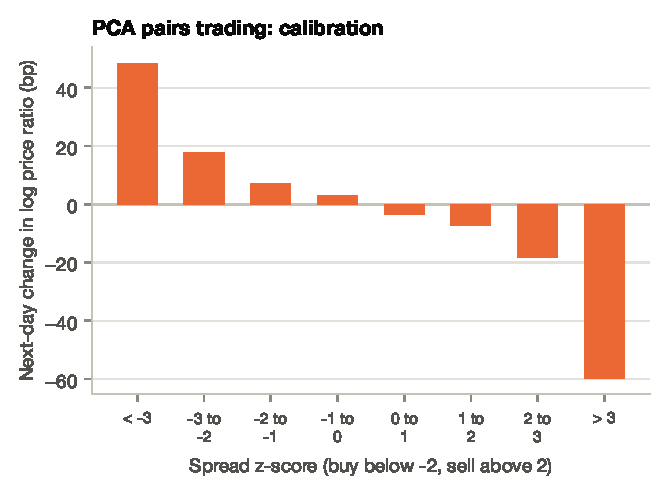
\includegraphics[width=0.65\textwidth]{figures/calibration_pairs.pdf}
\caption{Calibration of PCA pairs trading: next-day change in the pair log price ratio by spread z-score.}
\label{fig:calibration-pairs}
\end{figure}

\begin{figure}[!htbp]
\centering
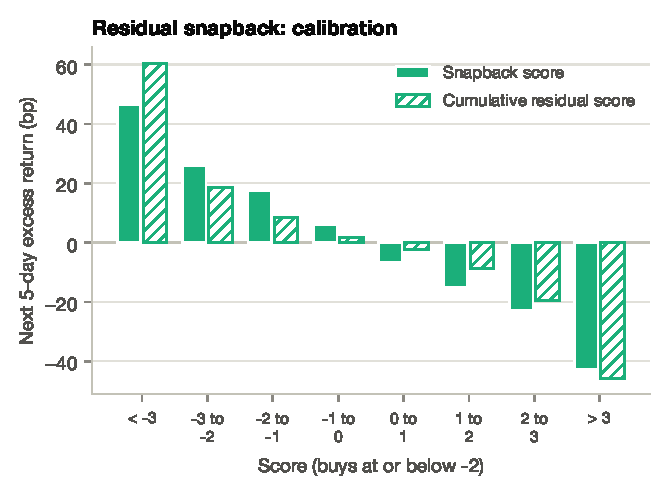
\includegraphics[width=0.65\textwidth]{figures/calibration_snap.pdf}
\caption{Calibration of residual snapback (Tables~\ref{tab:calibration-snap} and~\ref{tab:calibration-cumulative}): next 5-day excess return by snapback score (solid) and by cumulative residual score (hatched).}
\label{fig:calibration-snap}
\end{figure}

\begin{figure}[!htbp]
\centering
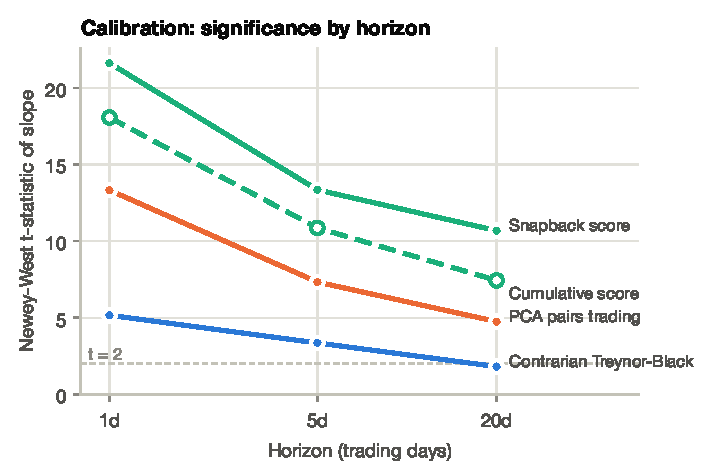
\includegraphics[width=0.65\textwidth]{figures/calibration_slopes.pdf}
\caption{Newey--West $t$-statistic of each signal's slope by horizon (Table~\ref{tab:calibration-slopes}); the cumulative residual score is dashed. The gray dashed line marks $t = 2$. The $t$-statistics are comparable across strategies even though the slopes are in different units.}
\label{fig:calibration-slopes}
\end{figure}

\subsection{Holdout}
\label{sec:holdout}

To check that our design choices are not overfit, we treat 2018--2023 as a holdout. Any choice is made using only 2002--2017 data and then evaluated once on the holdout.

\begin{table}[!htbp]
\centering
\caption{Selection period vs.\ holdout (Sharpe ratios, 5bp fees).}
\label{tab:holdout}
\begin{adjustbox}{max width=\linewidth}
\begin{tabular}{llrr}
\toprule
Strategy & Choice & 2002--2017 & 2018--2023 \\
\midrule
Treynor--Black & Default settings & 1.08 & 0.40 \\
& Best setting on 2002--2017 (alpha window 60) & 1.13 & 0.83 \\
& Best $K$ on 2002--2017 ($K = 20$) & 1.11 & 0.63 \\
Pairs trading & Default settings & 1.04 & 1.15 \\
& Best setting on 2002--2017 (spread window 20) & 1.63 & 1.05 \\
& Best $K$ on 2002--2017 ($K = 15$) & 1.41 & 0.58 \\
Snapback, long only & Default settings & 0.83 & 0.62 \\
& Best setting on 2002--2017 (1 signal day) & 1.23 & 0.69 \\
& Best $K$ on 2002--2017 ($K = 5$, the default) & 0.91 & 0.62 \\
& Best hedge mix on 2002--2017 (dynamic) & 1.06 & 0.51 \\
Snapback, fully hedged & Default settings & 0.87 & 0.59 \\
& Best setting on 2002--2017 (1 signal day) & 1.71 & 1.03 \\
& Best $K$ on 2002--2017 ($K = 3$) & 0.98 & 0.79 \\
\midrule
Following alpha (no fees) & Sign check & $-1.63$ & $-0.77$ \\
\bottomrule
\end{tabular}
\end{adjustbox}
\\[4pt]
\small Default, best-setting and hedge-mix rows use the common period of the parameter variants, starting December 2003 (March 2004 for snapback). Best-$K$ rows start in 2002, so the $K = 5$ row differs slightly from the default row.
\end{table}

\begin{figure}[!htbp]
\centering
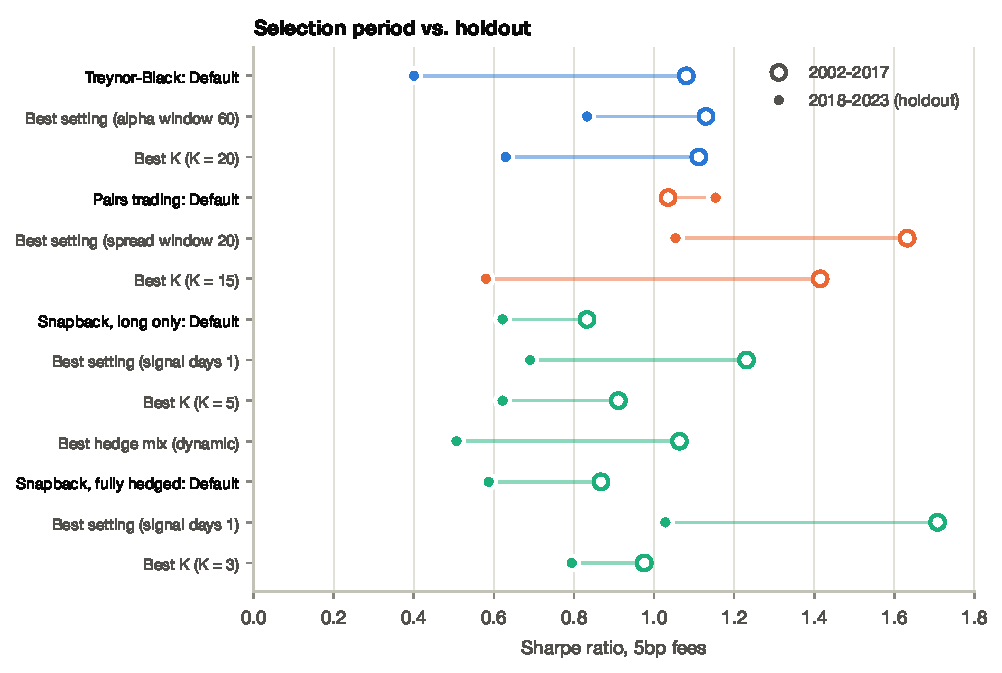
\includegraphics[width=0.85\textwidth]{figures/holdout.pdf}
\caption{Selection period vs.\ holdout (Table~\ref{tab:holdout}): Sharpe ratio with 5bp fees in 2002--2017 (hollow) and in the 2018--2023 holdout (filled). The no-fee sign check is omitted.}
\label{fig:holdout}
\end{figure}

Four results stand out. First, the contrarian direction is justified using the selection period alone: following alpha loses money in 2002--2017 (Sharpe $-1.63$), so reversing the sign was not chosen by looking at the full sample. Second, pairs trading holds up in the holdout (Sharpe 1.15, versus 1.04 before). Optimizing its parameters on the selection period did \emph{not} help: every optimized choice did worse in the holdout than the defaults, the classic signature of overfitting. Third, Treynor--Black weakens substantially in the holdout (Sharpe 0.40 with default settings), consistent with the decline in its second-half performance in Table~\ref{tab:regime}.

Fourth, residual snapback weakens in the holdout but less than Treynor--Black (0.62 long only and 0.59 hedged, from 0.83 and 0.87). Unlike for the other two strategies, some choices made on the selection period carried over. The one-day signal beat the default in the holdout in both versions (0.69 vs.\ 0.62 long only, 1.03 vs.\ 0.59 hedged), and $K = 3$ helped the hedged version (0.79). The best hedge mix on 2002--2017, the dynamic volatility mix, did not: it reached only 0.51 in the holdout, below the long-only default. Even where choices carried over, the holdout gains were smaller than the selection-period gains (for the one-day signal, $+0.07$ vs.\ $+0.40$ long only and $+0.44$ vs.\ $+0.84$ hedged), so part of the apparent improvement is overfitting.

\subsection{Number of factors $K$}

Finally, we re-run all three strategies for $K \in \{1, 2, 3, 5, 8, 10, 15, 20\}$, both out-of-sample and in-sample. In the in-sample version, the PCA and the alphas are estimated once on the full 2000--2023 sample and then traded over the same period, which introduces look-ahead bias. For residual snapback, the in-sample version computes each day's residual from the full-sample coefficients.

\begin{table}[!htbp]
\centering
\caption{Sharpe ratios by number of factors $K$.}
\label{tab:k}
\begin{adjustbox}{max width=\linewidth}
\begin{tabular}{rrrrrrrr}
\toprule
& \multicolumn{4}{c}{Treynor--Black} & \multicolumn{3}{c}{Pairs trading} \\
\cmidrule(lr){2-5} \cmidrule(lr){6-8}
& \multicolumn{2}{c}{Out-of-sample} & \multicolumn{2}{c}{In-sample} & \multicolumn{2}{c}{Out-of-sample} & In-sample \\
\cmidrule(lr){2-3} \cmidrule(lr){4-5} \cmidrule(lr){6-7}
$K$ & No fees & 5bp & Contrarian & Follow $\alpha$ & No fees & 5bp & No fees \\
\midrule
1 & 0.95 & 0.68 & $-1.54$ & 1.54 & 0.78 & 0.52 & 0.62 \\
2 & 0.86 & 0.54 & $-2.12$ & 2.12 & 1.39 & 1.11 & 0.69 \\
3 & 0.87 & 0.51 & $-2.13$ & 2.13 & 1.13 & 0.86 & 1.13 \\
5 & 1.31 & 0.85 & $-2.18$ & 2.18 & 1.45 & 1.17 & 1.93 \\
8 & 1.46 & 0.92 & $-2.76$ & 2.76 & 1.41 & 1.09 & 2.18 \\
10 & 1.49 & 0.91 & $-2.77$ & 2.77 & 1.53 & 1.18 & 2.40 \\
15 & 1.58 & 0.94 & $-3.29$ & 3.29 & 1.51 & 1.14 & 2.39 \\
20 & 1.66 & 0.96 & $-3.42$ & 3.42 & 1.60 & 1.18 & 2.15 \\
\bottomrule
\end{tabular}
\end{adjustbox}
\end{table}

\begin{figure}[!htbp]
\centering
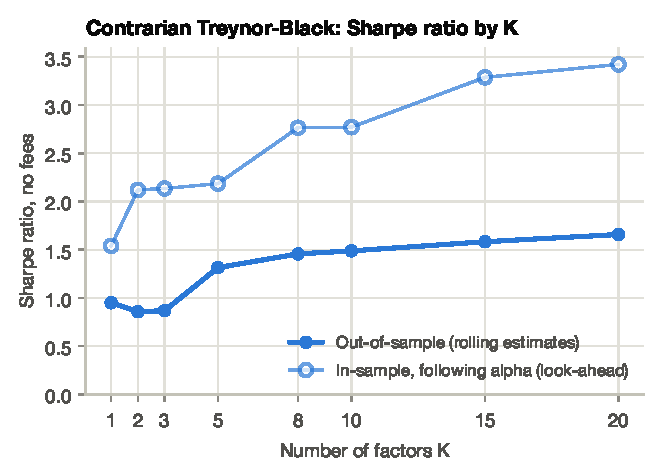
\includegraphics[width=0.65\textwidth]{figures/k_sweep_tb.pdf}
\caption{Sharpe ratio (no fees) of Contrarian Treynor--Black by number of factors $K$, out-of-sample vs.\ in-sample. The in-sample version follows alpha rather than trading against it.}
\label{fig:k-tb}
\end{figure}

\begin{figure}[!htbp]
\centering
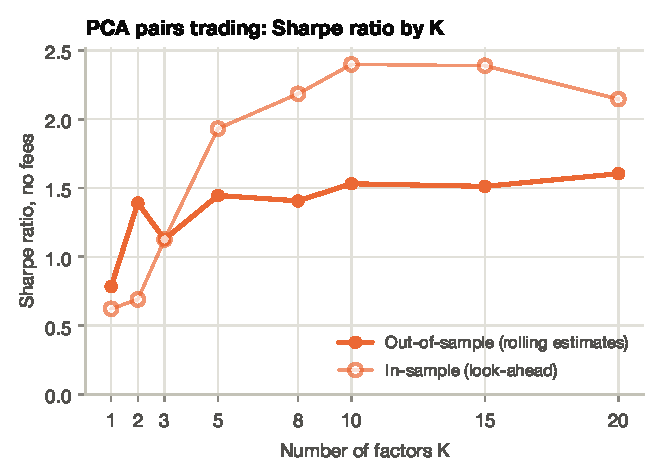
\includegraphics[width=0.65\textwidth]{figures/k_sweep_pairs.pdf}
\caption{Sharpe ratio (no fees) of PCA pairs trading by number of factors $K$, out-of-sample vs.\ in-sample.}
\label{fig:k-pairs}
\end{figure}

\begin{table}[!htbp]
\centering
\caption{Sharpe ratios by number of factors $K$: residual snapback.}
\label{tab:k-snap}
\begin{adjustbox}{max width=\linewidth}
\begin{tabular}{rrrrrrr}
\toprule
& \multicolumn{3}{c}{Long only} & \multicolumn{3}{c}{Fully hedged} \\
\cmidrule(lr){2-4} \cmidrule(lr){5-7}
& \multicolumn{2}{c}{Out-of-sample} & In-sample & \multicolumn{2}{c}{Out-of-sample} & In-sample \\
\cmidrule(lr){2-3} \cmidrule(lr){5-6}
$K$ & No fees & 5bp & No fees & No fees & 5bp & No fees \\
\midrule
1 & 1.01 & 0.81 & 1.03 & 1.41 & 0.89 & 1.40 \\
2 & 1.02 & 0.82 & 1.01 & 1.31 & 0.78 & 1.52 \\
3 & 1.03 & 0.82 & 1.07 & 1.53 & 0.91 & 1.64 \\
5 & 1.03 & 0.82 & 1.18 & 1.38 & 0.76 & 1.84 \\
8 & 1.00 & 0.79 & 1.13 & 1.50 & 0.77 & 1.86 \\
10 & 0.98 & 0.77 & 1.16 & 1.38 & 0.65 & 1.93 \\
15 & 1.01 & 0.80 & 1.12 & 1.01 & 0.29 & 1.88 \\
20 & 0.98 & 0.77 & 1.12 & 0.46 & $-0.21$ & 1.97 \\
\bottomrule
\end{tabular}
\end{adjustbox}
\end{table}

\begin{figure}[!htbp]
\centering
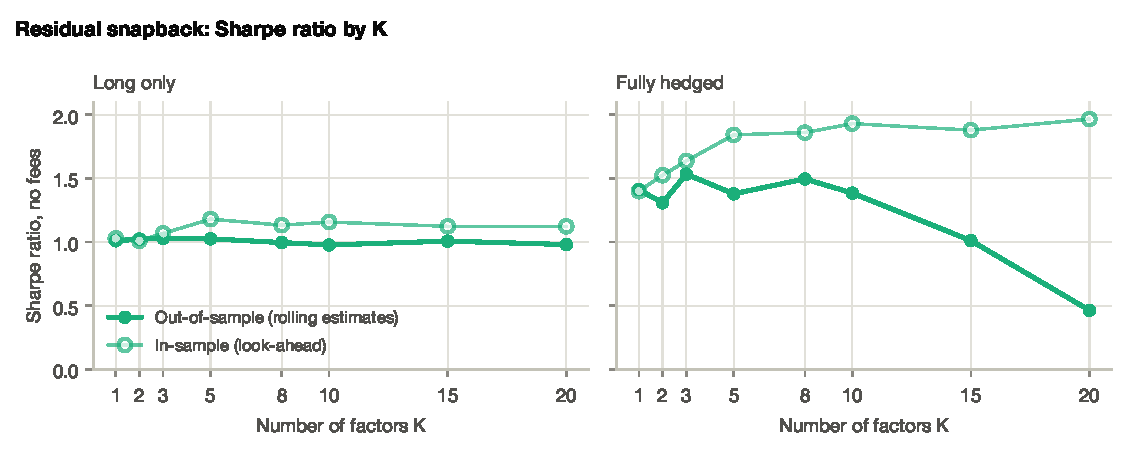
\includegraphics[width=0.65\textwidth]{figures/k_sweep_snap.pdf}
\caption{Sharpe ratio (no fees) of residual snapback by number of factors $K$, out-of-sample vs.\ in-sample, long only (left) and fully hedged (right).}
\label{fig:k-snap}
\end{figure}

\paragraph{In-sample vs.\ out-of-sample.} The difference is dramatic (Figures~\ref{fig:k-tb} and~\ref{fig:k-pairs}). In-sample, following alpha appears highly profitable, with Sharpe ratios of 2 to 3.4 that rise as more factors are added. This is look-ahead bias: the full-sample alpha is estimated from the very returns being traded, so stocks with high alpha mechanically earned high returns over the period. Out-of-sample, the same signal points the \emph{opposite} way: high past alpha predicts low future returns. An in-sample assessment would not just overstate performance; it would recommend the wrong strategy. Pairs trading is also inflated in-sample (Sharpe up to 2.4 vs.\ about 1.5 out-of-sample), though its direction is unchanged. Long-only residual snapback is the least affected (Figure~\ref{fig:k-snap}): its in-sample Sharpe ratios exceed out-of-sample ones by at most 0.18. Its signal is a short-lived residual relative to a stock's own recent volatility, which full-sample coefficients barely change, rather than an estimate of the long-run alpha that look-ahead contaminates directly. The hedged version is affected much more, increasingly so as $K$ grows (1.84 vs.\ 1.38 at $K = 5$, 1.97 vs.\ 0.46 at $K = 20$). Its hedge relies on the betas, and full-sample betas describe the factor exposures over the very period being traded, so in-sample the hedge removes factor risk almost perfectly. Out-of-sample, each extra factor adds another set of estimated betas to hedge against, and their estimation error accumulates.

\paragraph{Which $K$ works best?} Out-of-sample, performance improves up to roughly $K = 5$--$8$ and then levels off, especially after fees. For Treynor--Black, the Sharpe ratio after fees is 0.85 at $K = 5$ and only 0.96 at $K = 20$. For pairs trading, every $K \ge 2$ gives a Sharpe ratio between 0.86 and 1.18 after fees. Picking $K$ by its past performance also did not carry over to the holdout for Treynor--Black or pairs trading (Table~\ref{tab:holdout}). Long-only snapback is insensitive to $K$ (0.77--0.82 after fees for every value). The hedged version prefers \emph{few} factors: after fees it does best at $K = 1$--$3$ (0.78--0.91) and deteriorates beyond $K = 8$ (0.29 at $K = 15$, $-0.21$ at $K = 20$), because each extra factor to neutralize forces the weights further from the signal and adds estimation noise to the hedge. We therefore keep $K = 5$ for all three strategies: it captures most of the benefit, and larger values add estimation noise without a reliable improvement.

\section{Conclusion}

All three PCA strategies are profitable out-of-sample and after transaction costs, but they differ in robustness. Contrarian Treynor--Black shows that estimated alphas reverse rather than persist. It is factor neutral by construction (market beta 0.04) and performs best in crises, but it is concentrated in 2008--09, sensitive to trading costs, and has weakened since 2013. PCA pairs trading is the most robust strategy: it is profitable in 21 of 22 years, well calibrated, insensitive to its parameters, and stronger in the 2018--2023 holdout than before it. Residual snapback has the strongest signal of the three, with stocks that fall well short of the factor model's prediction reliably outperforming over the next one to twenty days. Its implementation captures only part of that signal. The long-only version mostly earns the market return (beta 1.08, the same Sharpe ratio as an equal-weight benchmark), and the fully hedged long-short version, comparable to the other two strategies, has a Sharpe ratio of 1.38 before fees but trades about 100 times a year and gives up almost half of its edge to costs. Both weaken in the holdout, and the hedged version's edge has faded since 2013. Measuring the shortfall cumulatively rather than over three days helps most: with the same trading rules, the cumulative residual score raises the long-short Sharpe ratio after fees to 1.76 (1.26 in the holdout) and keeps 1.07 when trades are executed a day late. A daily version of the same signal reaches 3.01, but it collapses to 0.25 with a one-day delay. Most of its profit comes from next-day price reversals that a real trader could probably not capture. The contrast between in-sample and out-of-sample results shows why rolling estimation matters. Estimating the model on the full sample does not merely inflate performance; for Treynor--Black it reverses the conclusion about which way to trade.


% BEGIN ARCHIVED: Earlier residual-strategy draft; integrated treatment is in Section 4
% ARCHIVE 
% ARCHIVE \quad
% ARCHIVE 
% ARCHIVE Strategy 3: Residual Mean Reversion Strategy
% ARCHIVE 
% ARCHIVE The underlying strategy for the residual mean reversion strategy has to do with the underlying belief that when stocks move down on d more than what we had predicted from the data from days 1,..., d-1, then we should buy these particular stocks as we believe that the market has undervalues/overreacted to these stocks (and that they have higher relative expected value to assets that have moved as expected in our regression or assets that have moved higher than our prediction from the regression. The difference between this strategy and the Treynor black method is the fact that Treynor Black relies on inspection on the alpha parameter while the residual snapback strategy relies on buying stocks that we believe are relatively undervalued due to an overreaction in the markets.
% ARCHIVE 
% ARCHIVE For Treynor–Black, we have used a 250-day regression window since the estimated alpha from this data directly determines the trading signal and a longer window of data would gives us many more observations and would reduce the influence of a  anomalies in the data. 
% ARCHIVE 
% ARCHIVE However, for residual snapback, the regression serves a different purpose. This regression is supposed to give us a baseline/prior against we need to measure these recent unexpected returns. A shorter window such as a 100-day window lets that baseline adapt more quickly to recent changes in the stock’s factor exposures, while also at the cost of estimates with higher standard devations.  However, due to the short term edge We therefore use 100 days for snapback as a design choice suited to its short-horizon signal.
% ARCHIVE \quad
% ARCHIVE 
% ARCHIVE Now, to understand the "signal" of the residual between the actual daily return compared to the regressions predictions, we need to get an understanding of how much of a deviation/size of residual is normal for a particular stock. For example, if a particular stock barely deviates from the regression prediction and then randomly is 5 percent different than what the regression predicts would have a different signal than a stock that on average has a 5 percent deviation from the regression prediction. To do this, we look at the last 60 trading days and fit the regression model to 1 day less than our current day. Then, we calculate the residuals on those 60 days. After we have these residuals, we use these 60 data points to get a sample variance for the residual as well as a sample mean. Then, we examine how the next three days of trading looks like after we have out 100 days of data. After normalizing the average residual by transforming it into a z score, we get a heuristic/z-score statistic for how much the stock has gone down compared to its "fair value." Although "fair value" is not the correct depicition since we have no way of understanding what is a "fair value." 
% ARCHIVE 
% ARCHIVE \[
% ARCHIVE \mathrm{Score}_{i,t}
% ARCHIVE =
% ARCHIVE \frac{\displaystyle\sum_{k=0}^{2}\varepsilon_{i,t-k}}
% ARCHIVE      {\sqrt{3}\,\widehat{\sigma}_{i,t}},
% ARCHIVE \qquad
% ARCHIVE \widehat{\sigma}_{i,t}
% ARCHIVE =
% ARCHIVE \sqrt{\frac{1}{59}
% ARCHIVE \sum_{k=3}^{62}
% ARCHIVE \left(\varepsilon_{i,t-k}-\overline{\varepsilon}_{i,t}\right)^2},
% ARCHIVE \qquad
% ARCHIVE \overline{\varepsilon}_{i,t}
% ARCHIVE =
% ARCHIVE \frac{1}{60}\sum_{k=3}^{62}\varepsilon_{i,t-k}.
% ARCHIVE \]
% ARCHIVE 
% ARCHIVE Note that the numerator here in the score function is the sum of the three errors (the days 1 day 2 day and 3 day after the 100 previous days of regression and the 60 previous days of understanding how our model is calibrated.) A negative value in the error refers to the stock underperforming the return compared to what our factor model was predicting over those three days. On the other hand, a positive value means that we thought that the market price has "overshot" what the factor model would have predicted. If we assume that the expected value of each of these errors is 0 (the factor model is an unbiased estimator of what the price of a stock should be condicitioned upon the rest of the market prices), then we essentially know that the sum in the numerator is how much the price and the "condiitonal mean disagree." Now, the denominator of the stock is used to "standardize" the error, as we have mentioned earlier. We have estimated summa i,t hat from the previous 60 days of trading data and then we know that the sum of three random variables has a variance that is 3 times a single one, since the standard deviation is sqrt of variance, then we know that the sum of three std devs is equivalent in expansion to sqrt(3) * standard dev which is why we divide by sqrt(3) in the denominator.
% ARCHIVE (An assumption that we are making when dividing by sqrt(3) is that the residuals are uncorrelated, which may be a strech given that this "error" is hypothesized to be due to irrational market sentiment, which would likely presist and be correlated throughout the three days. If we were to think about this strategy more, one way to add complexity would be to alter the denominator to match this. However, since this score applied to all of the stocks in our portfolio, it is likely not that important if our signal is supposed to be multiplied by a particular magnitude that is constant/not dependent on our stock (given that a signal is only important as it has relative information, meaning that its used to compare two stocks). 
% ARCHIVE 
% ARCHIVE The second expression is how we have calulated the standard deviation. Hopefully, the average error is ei,t which would mean that we predicted the error well and then we are only dividing by 59 instead of 60 because the expression is sqrt(1/(n-1) * rss) for the sample standard deviation. 
% ARCHIVE 
% ARCHIVE Below here, I have also attached the 60-day residual mean across stocks, so that we can examine if it is true that that the regression model likely is an unbiased conditional estimate of a securities market price:  
% ARCHIVE 
% ARCHIVE 
% ARCHIVE \begin{figure}[H]
% ARCHIVE     \centering
% ARCHIVE     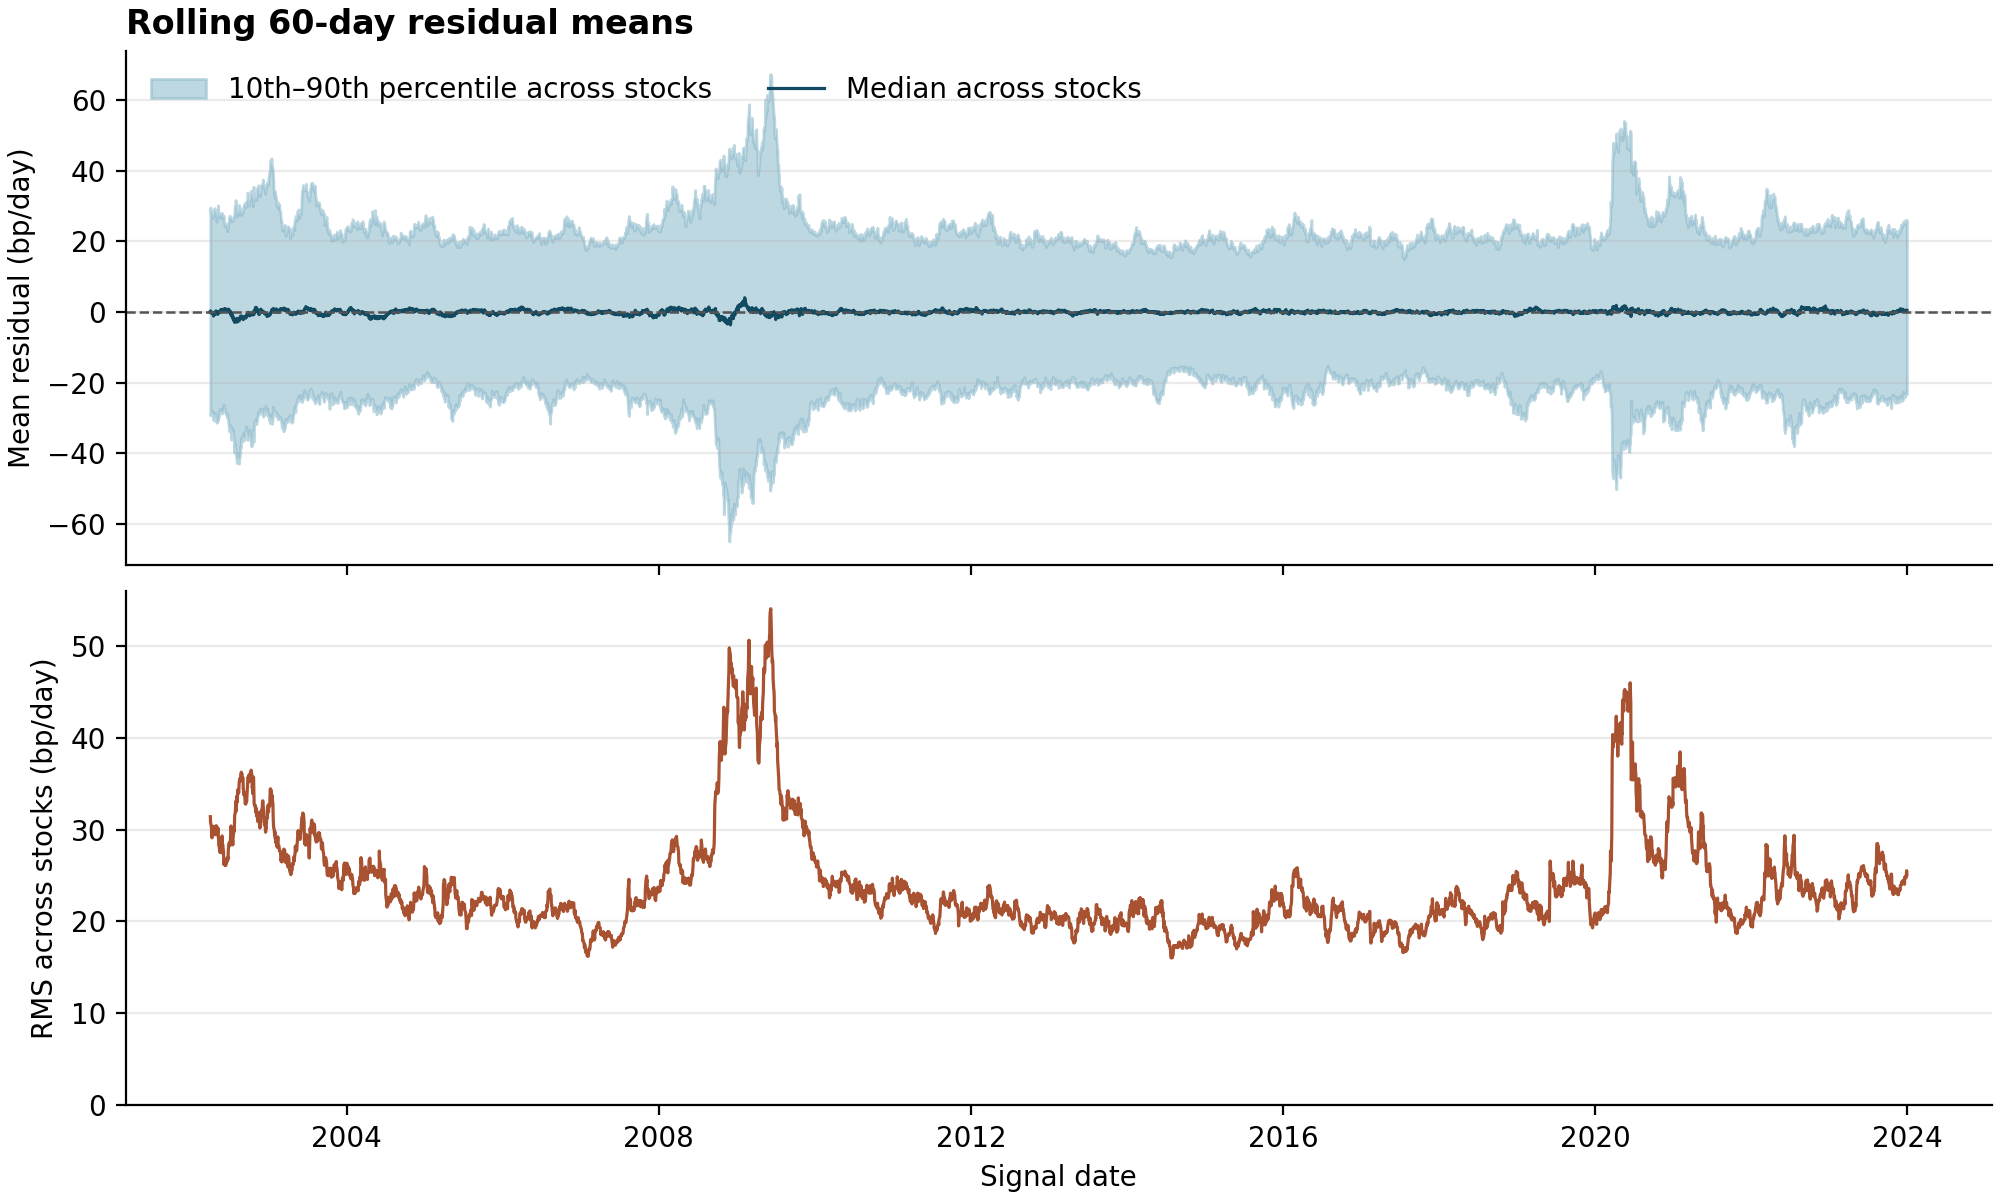
\includegraphics[width=0.5\linewidth]{errors.png}
% ARCHIVE     \caption{Enter Caption}
% ARCHIVE     \label{fig:}
% ARCHIVE \end{figure}
% ARCHIVE 
% ARCHIVE \begin{figure}[H]
% ARCHIVE     \centering
% ARCHIVE     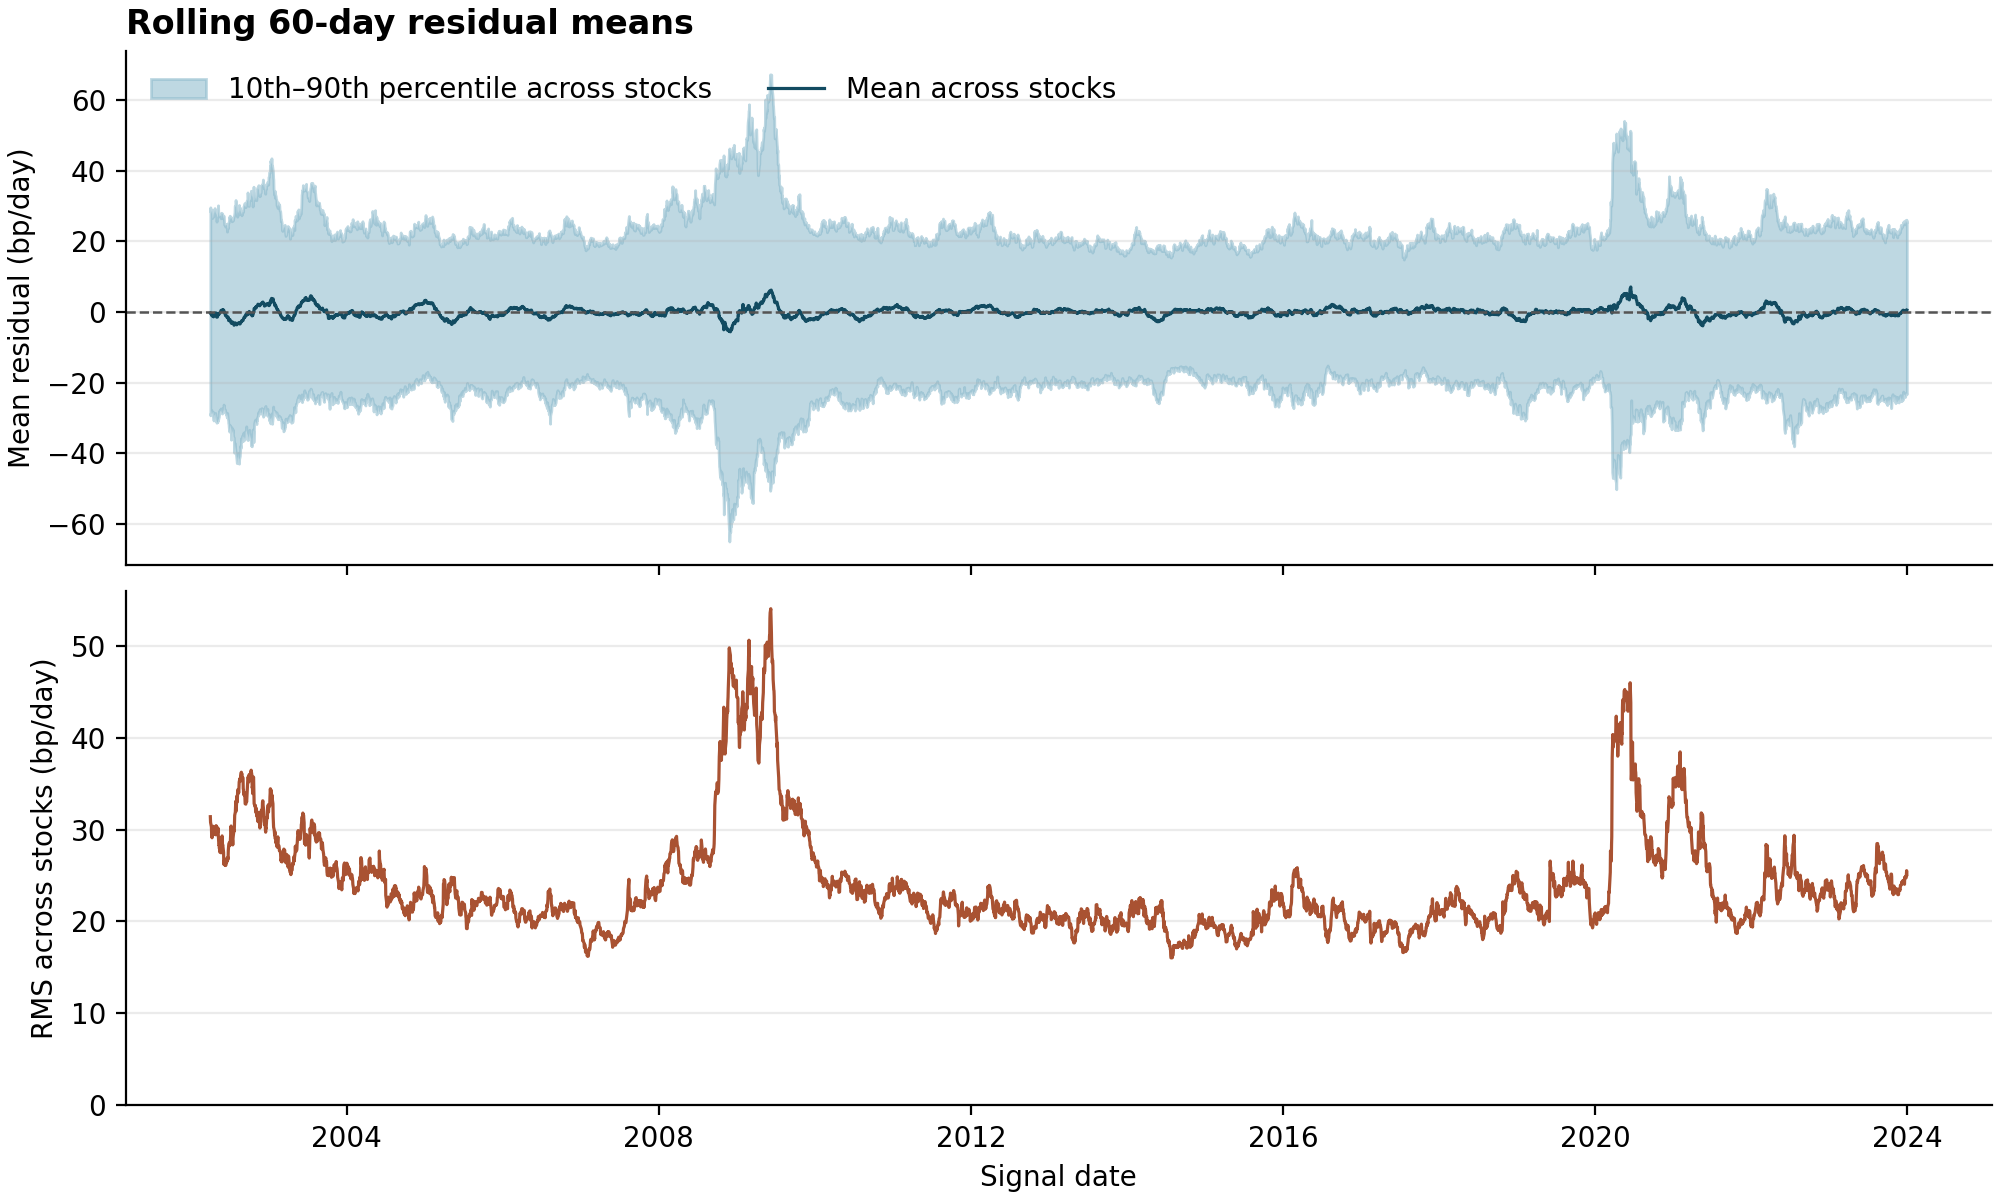
\includegraphics[width=0.5\linewidth]{erorrs_mean.png}
% ARCHIVE     \caption{Enter Caption}
% ARCHIVE     \label{fig:placeholder}
% ARCHIVE \end{figure}
% ARCHIVE 
% ARCHIVE 
% ARCHIVE Notice that after examining these figures, they show that the factor model has quite a small average signed error (0) across the stocks. 
% ARCHIVE  This suggests that when using the factor exposures and the regression used/fitted until the prior day, the model explains returns without a  tendency to overstate or understate them or understate them on average. 
% ARCHIVE 
% ARCHIVE 
% ARCHIVE  Trading Sub-Strategies:    
% ARCHIVE 
% ARCHIVE 
% ARCHIVE \paragraph{Naive residual snapback.}
% ARCHIVE 
% ARCHIVE On the last trading day of each week, we rank stocks by their residual
% ARCHIVE scores and select up to 20 stocks with "scores" of -2 or lower. If there are more than 20 stocks that have scores of -2 or lower, then we select the ones that have the lowest scores. If we have n stocks, we would go long in each stock with a proprtion of 1/n for each stock. If there are zero stocks that qualify, then we would hold all of our portfolio in cash. We re-evaluate our portfolio each trading day of the week by looking at the past 3 days, Wednesday throguh firsthand and the recalibrate our portfolio at the end of the week. 
% ARCHIVE 
% ARCHIVE \paragraph{Experimental Factor Hedging on Top of Naive Residual Snapback}
% ARCHIVE \begin{figure}[H]
% ARCHIVE     \centering
% ARCHIVE     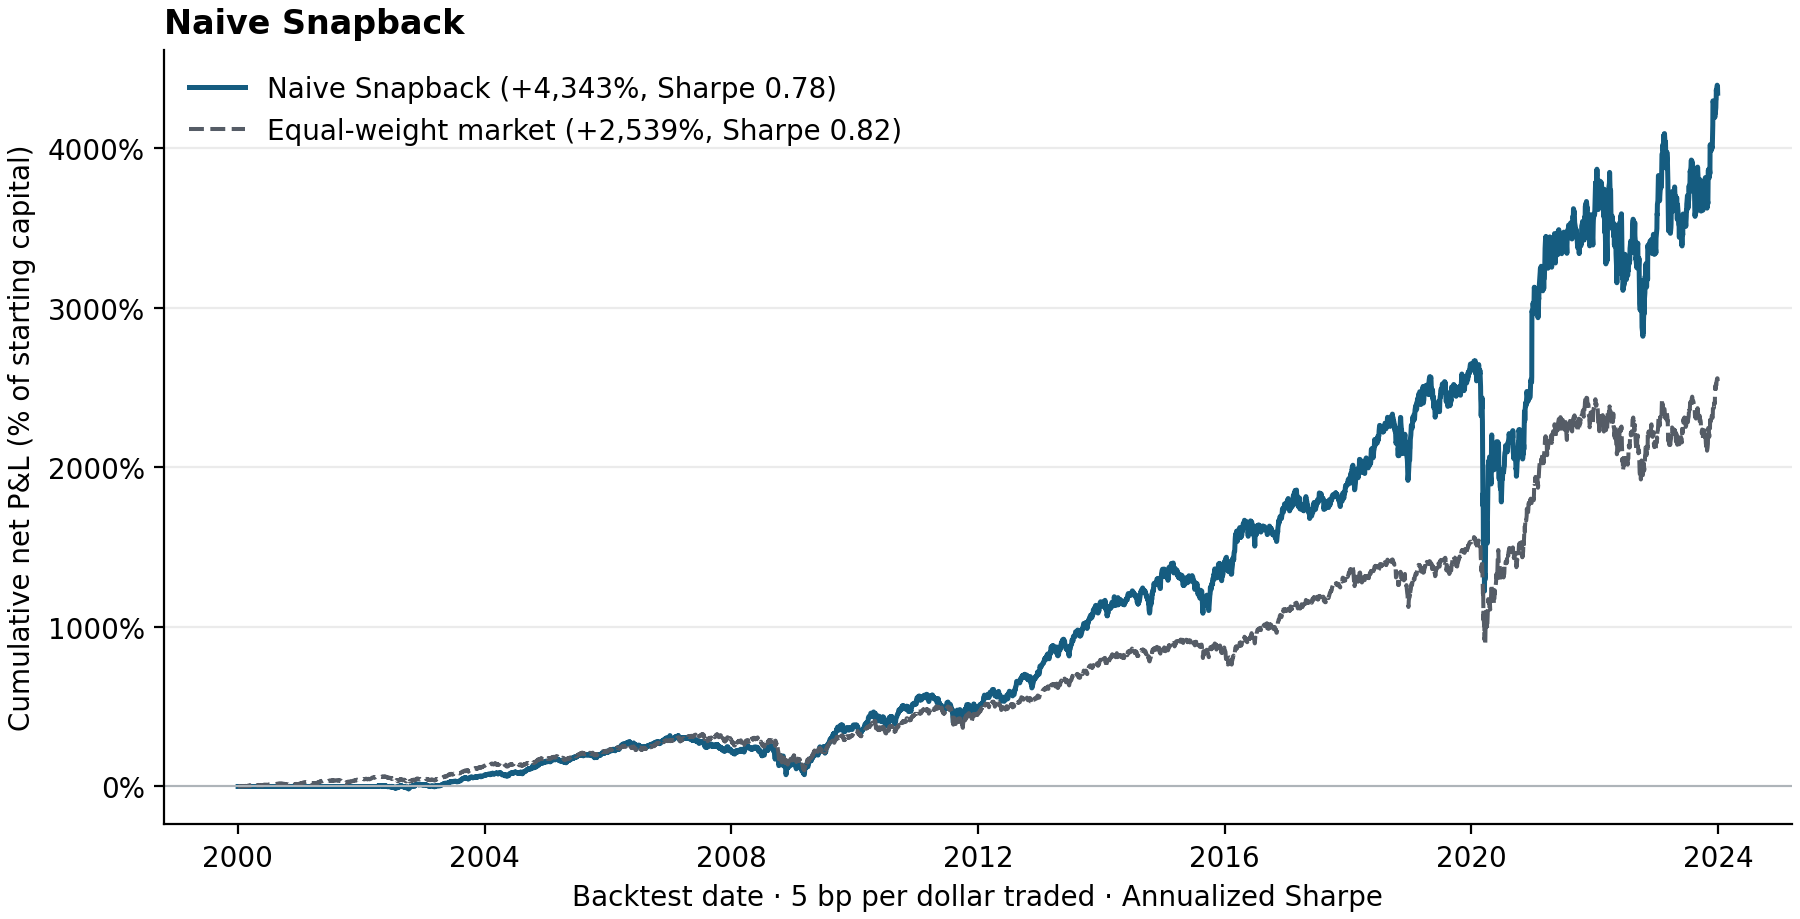
\includegraphics[width=0.5\linewidth]{naive_snapback.png}
% ARCHIVE     \caption{The naive}
% ARCHIVE     \label{fig:placeholder}
% ARCHIVE \end{figure}
% ARCHIVE 
% ARCHIVE 
% ARCHIVE 
% ARCHIVE 
% ARCHIVE 
% ARCHIVE \begin{figure}[H]
% ARCHIVE     \centering
% ARCHIVE     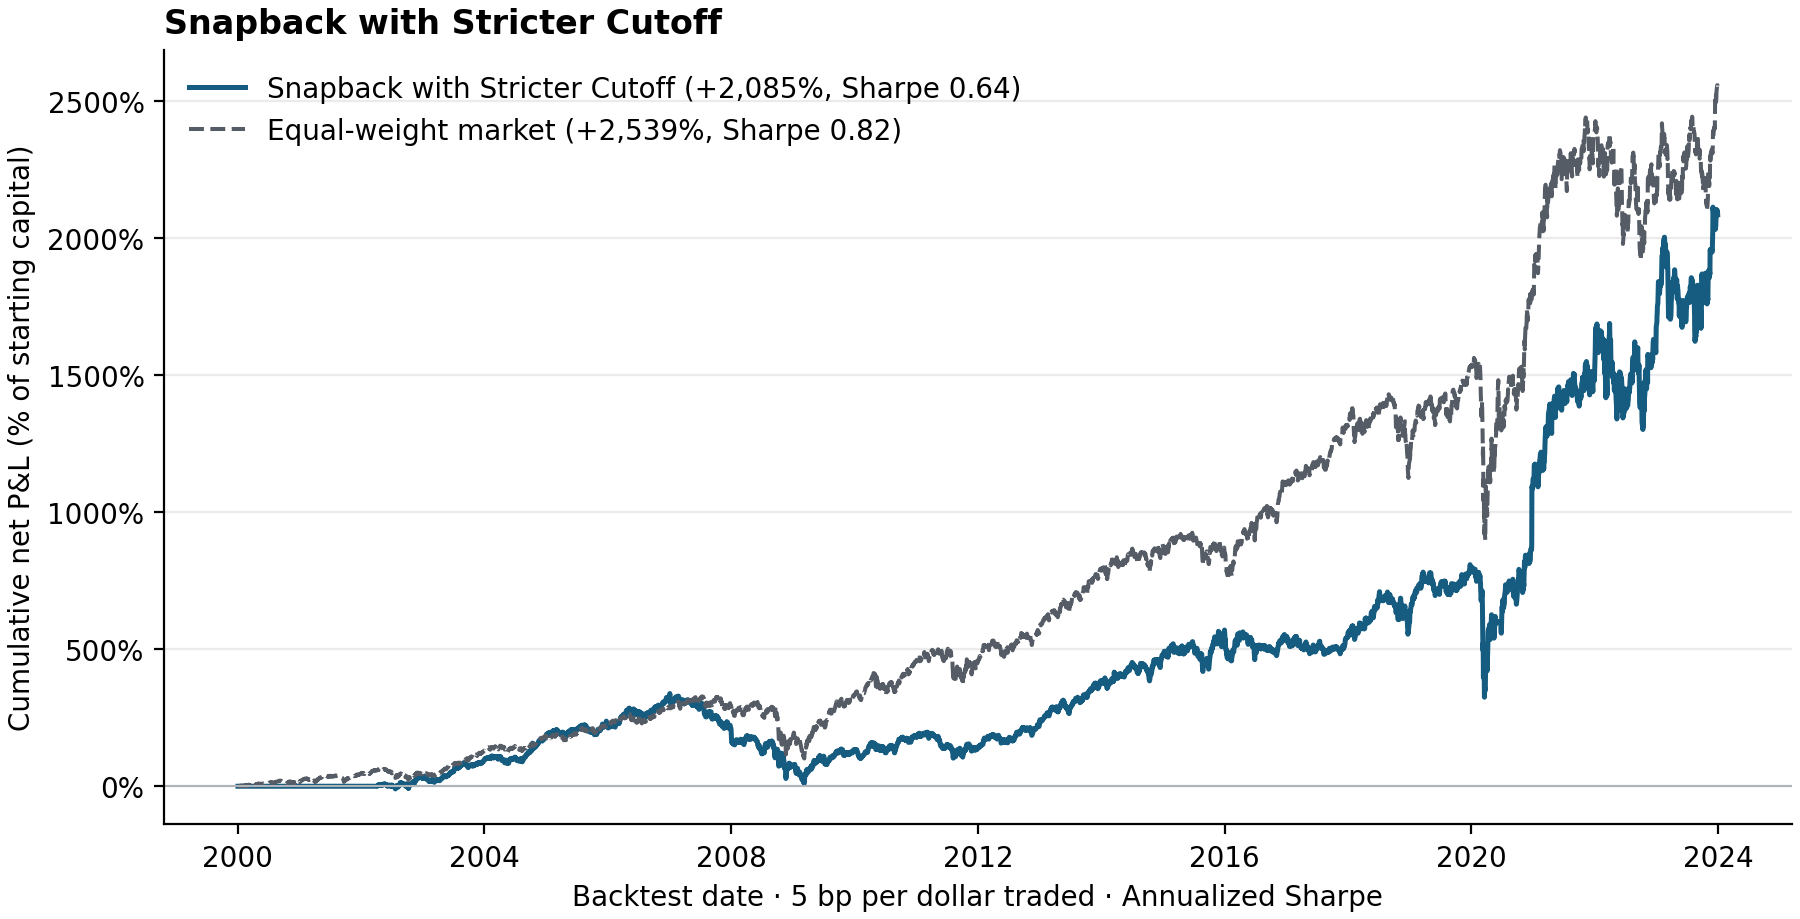
\includegraphics[width=0.5\linewidth]{stricter_cutoff.png}
% ARCHIVE     \caption{stricter cuttoff}
% ARCHIVE     \label{fig:placeholder}
% ARCHIVE \end{figure}
% ARCHIVE 
% ARCHIVE 
% ARCHIVE 
% ARCHIVE 
% ARCHIVE \begin{figure}[H]
% ARCHIVE     \centering
% ARCHIVE     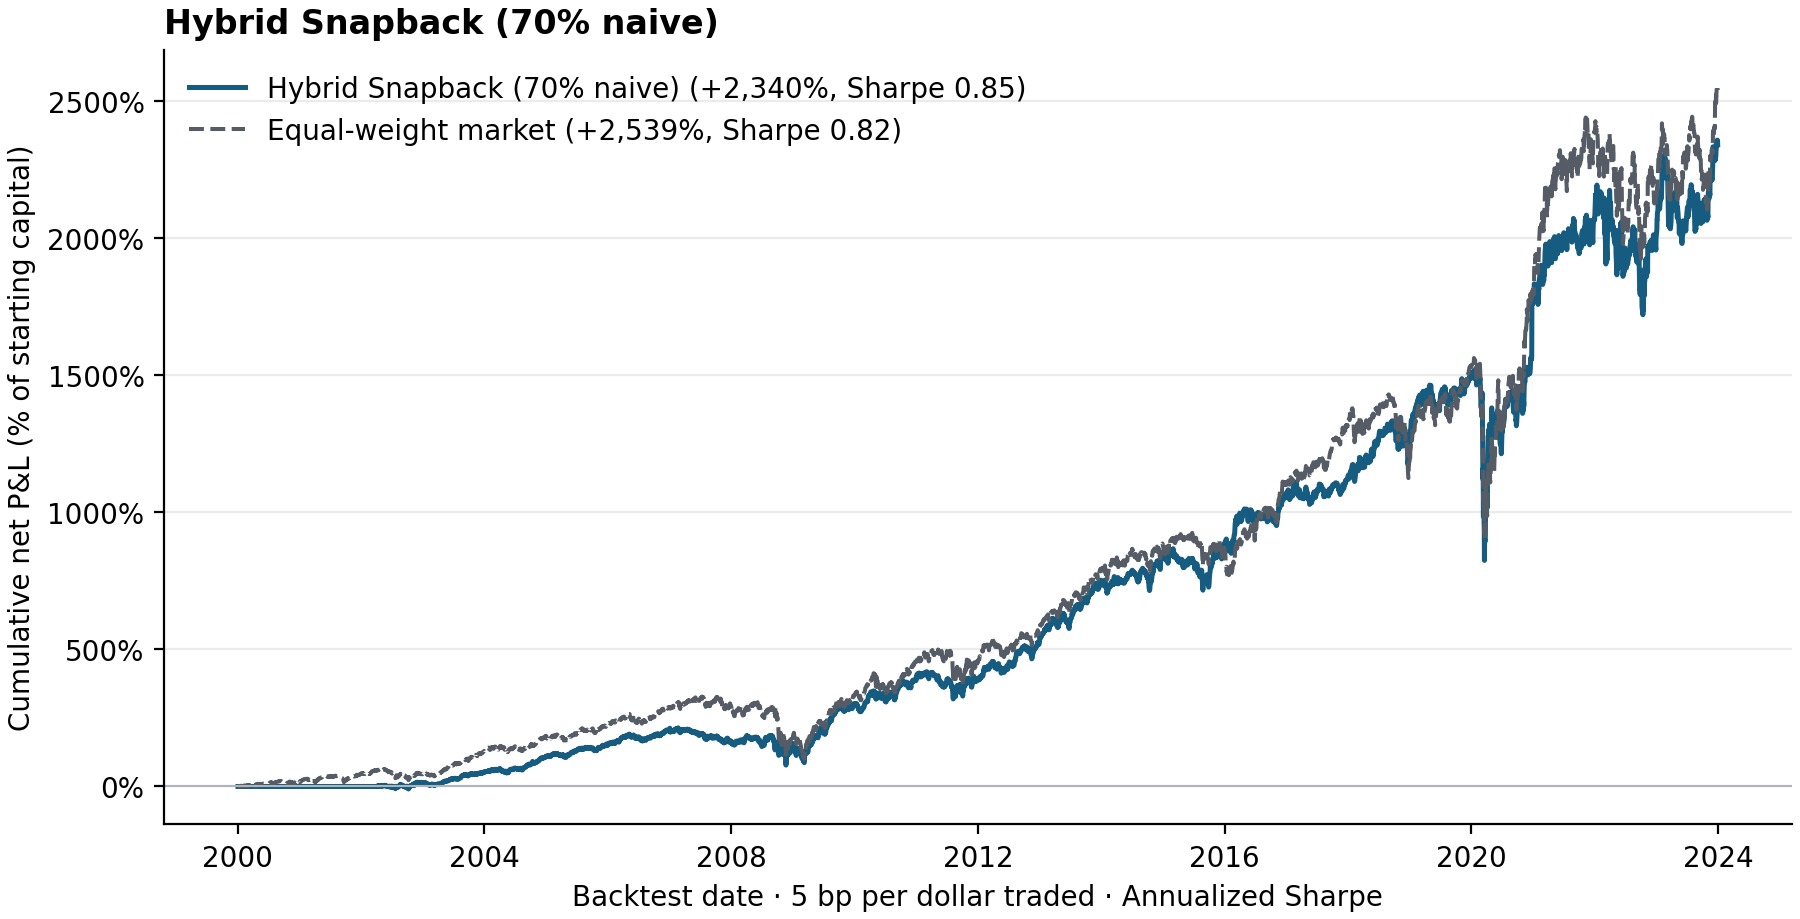
\includegraphics[width=0.5\linewidth]{70percentnaive_30percenthedged.png}
% ARCHIVE     \caption{70 percent hedged and 30 percent naive}
% ARCHIVE     \label{fig:placeholder}
% ARCHIVE \end{figure}
% ARCHIVE 
% ARCHIVE 
% ARCHIVE 
% ARCHIVE Although the signal may be choosing stocks that are expected to be higher than the market, it can still have exposures to those 5 PCA factors/vectors. For example, our portfolio could be heavily positively exposed to the 2nd principal component, if we have an equal weight long portfolio that is sensitive to these movements, then that would not be ideal. To hedge out our portfolio to these exposures, we can naively start with our selected group of stocks and adjust their weights. 
% ARCHIVE 
% ARCHIVE The fully hedged strategy aims to mitigate this risk by collecting the top 40 eligible stocks that have the "lowest scores" (meaning that they have moved downwards more than what we expect) and set these as our "long candidate space." Then, we take up to 40 stocks with the most positive scores as short candidates. The longs express the fact that we believe some of the candidates have moved too far down and should be worth more (with relation to the rest of the market) and the shorts we have are the stocks that we believe have moved too far up in relation to the other stocks in our portfolio space. We then start with target weights that would allow us to provide 50 percent of our capital to the shorts and 50 percent to the longs. 
% ARCHIVE 
% ARCHIVE %look into the below well
% ARCHIVE 
% ARCHIVE We can denote wt(0) denote these signed target
% ARCHIVE weights (which we have naivelly set it to be .5 * 1/(number of long candidates) for each vector entry that corresponds to the stock that has a negative stock and .5 * 1/n(number of short candidates) for a stock that corresponds to a positive score. Now, also let Bt be the matrix whose columns contain the five estimated PCA factor loadings for each selected stock.  Note that the dimension of B is 5 * (number of stocks that are both in the long or short candidate space). 
% ARCHIVE 
% ARCHIVE For any weight
% ARCHIVE vector wt, the portfolio's estimated factor exposures are
% ARCHIVE Btwt. We choose weights as close as possible to the
% ARCHIVE initial targets while imposing factor neutrality and preserving the
% ARCHIVE direction of each trade:
% ARCHIVE \[
% ARCHIVE \begin{aligned}
% ARCHIVE \min_{\mathbf{w}_t}\quad &
% ARCHIVE     \frac{1}{2}\|\mathbf{w}_t-\mathbf{w}^{(0)}_t\|_2^2 \\
% ARCHIVE \text{subject to}\quad &
% ARCHIVE     B_t\mathbf{w}_t=\mathbf{0}, \qquad
% ARCHIVE     \sum_i |w_{i,t}|=1,\\
% ARCHIVE &   w_{i,t}\geq 0 \quad \text{for long candidates},\\
% ARCHIVE &   w_{i,t}\leq 0 \quad \text{for short candidates}.
% ARCHIVE \end{aligned}
% ARCHIVE \]
% ARCHIVE 
% ARCHIVE \begin{figure}[H]
% ARCHIVE     \centering
% ARCHIVE     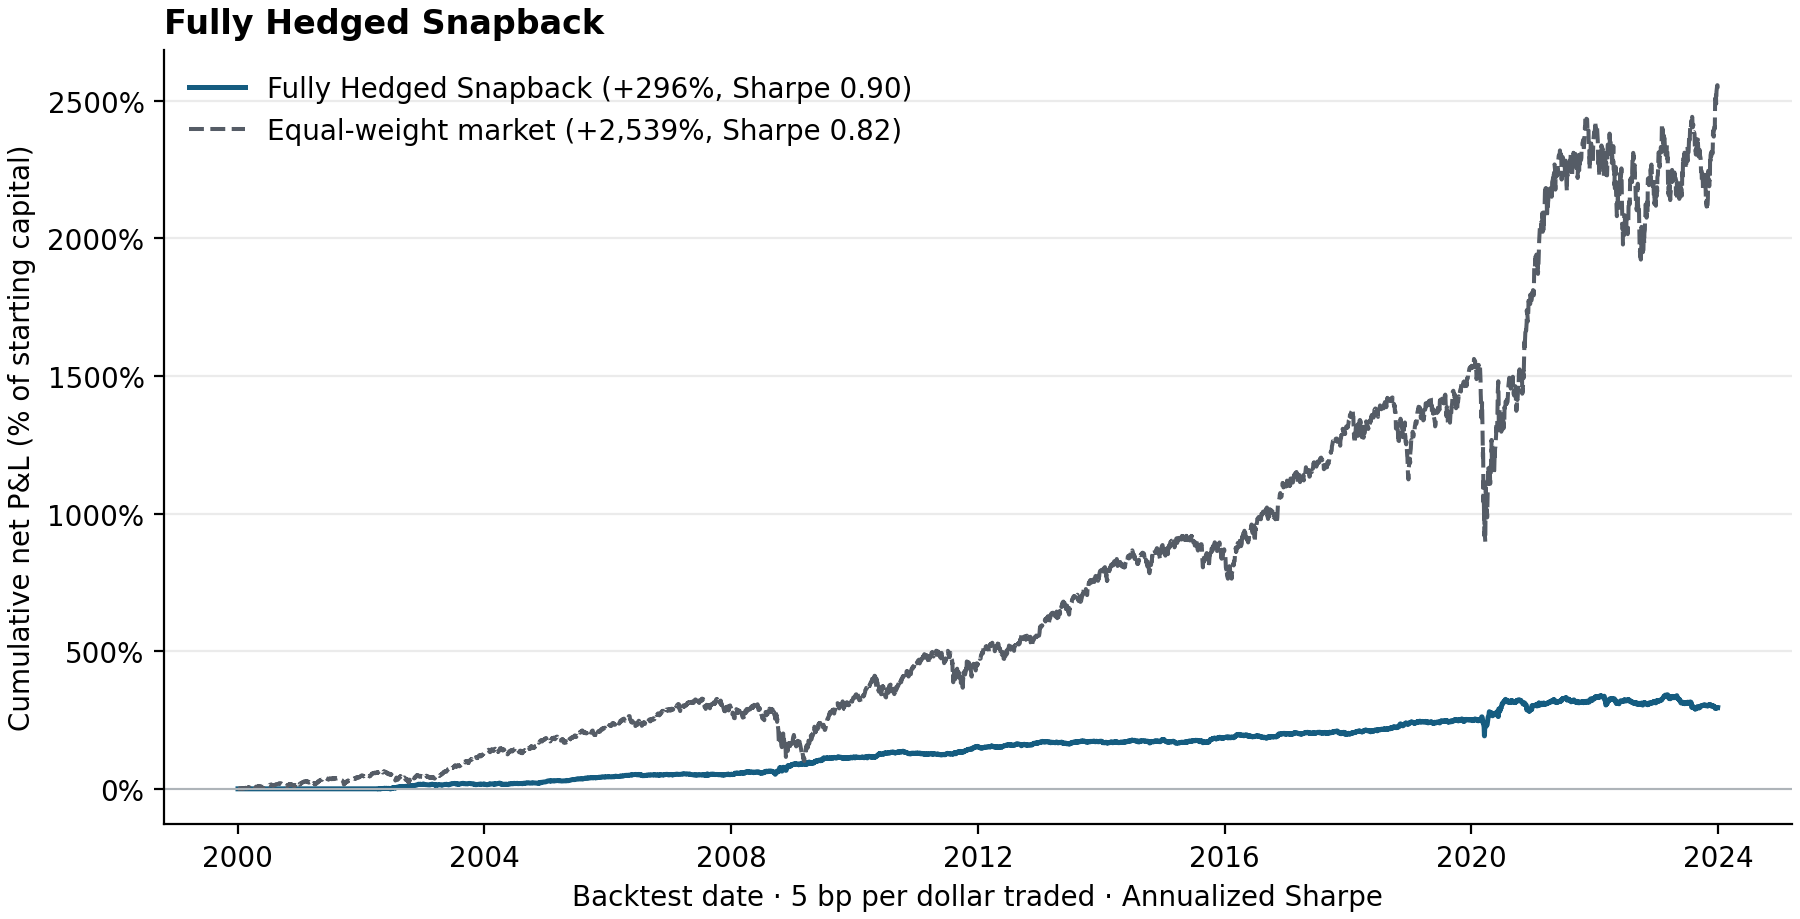
\includegraphics[width=0.5\linewidth]{fully_hedged.png}
% ARCHIVE     \caption{fully hedged portfolio}
% ARCHIVE     \label{fig:placeholder}
% ARCHIVE \end{figure}
% ARCHIVE 
% ARCHIVE After performing this strategy and keeping all other frameworks from the previous strategy the same, we get the following results: 
% ARCHIVE 
% ARCHIVE \begin{figure}[H]
% ARCHIVE     \centering
% ARCHIVE     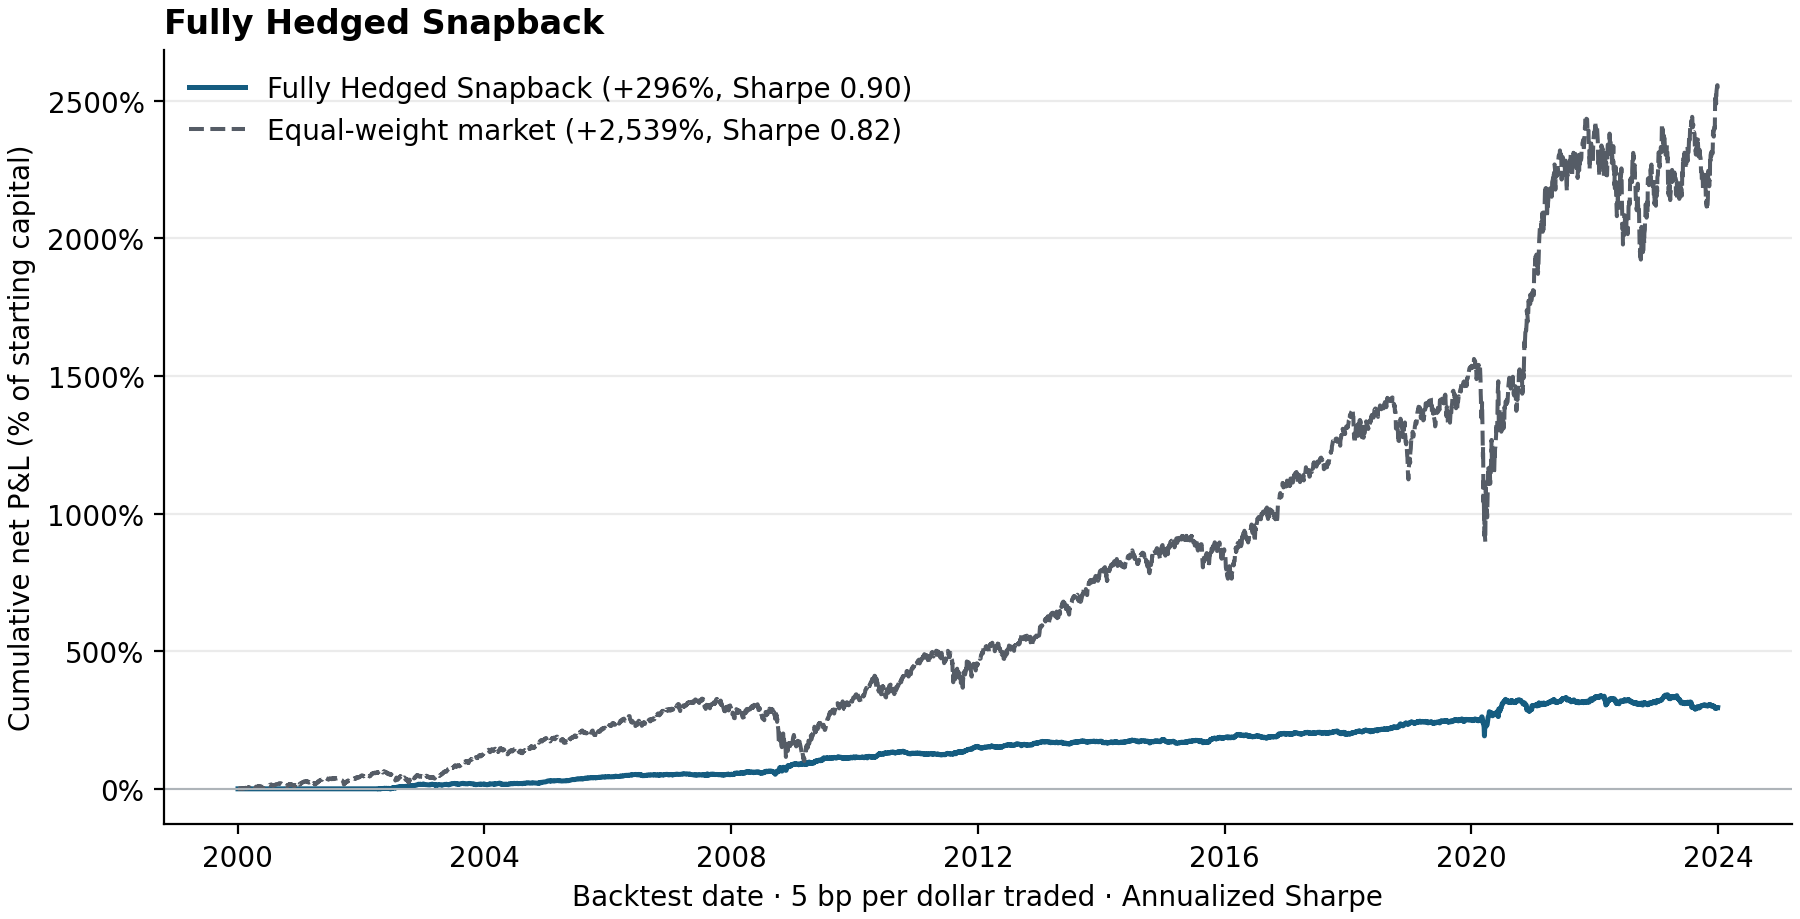
\includegraphics[width=0.5\linewidth]{fully_hedged.png}
% ARCHIVE     \caption{fully hedged portfolio}
% ARCHIVE     \label{fig:placeholder}
% ARCHIVE \end{figure}
% ARCHIVE 
% ARCHIVE \paragraph{Fixed-weight hybrid residual snapback.}
% ARCHIVE Our naive intitial Snapback portfolio gives full weight to (at most) 20 long-only
% ARCHIVE rebound signals, while the fully hedged portfolio offsets exposure to the five PCA factors by constructing the weights to meet a Principal component neutral portfolio. Now, what if we were to blend both these portfolios to retain the naive strategies upside (since this portfolio is known to perform better in terms of returns compared to market) while reducing exposure/risk through the hedged portfolio. 
% ARCHIVE 
% ARCHIVE We test whether blending the two
% ARCHIVE portfolios can retain some of the naive strategy's upside while
% ARCHIVE reducing its exposure to common factor moves.
% ARCHIVE 
% ARCHIVE 
% ARCHIVE %look into the below more: 
% ARCHIVE 
% ARCHIVE Essentially, we are keeping each of the two strategies exactly the
% ARCHIVE same. All we are doing is constructing both portfolios separately
% ARCHIVE and then combining their stock weights:
% ARCHIVE \[
% ARCHIVE     \mathbf{w}_t^{\mathrm{hybrid}}
% ARCHIVE     = \lambda\,\mathbf{w}_t^{\mathrm{naive}}
% ARCHIVE     + (1-\lambda)\,\mathbf{w}_t^{\mathrm{hedged}}.
% ARCHIVE \]
% ARCHIVE 
% ARCHIVE Our parameter that we have the freedom to change is ,
% ARCHIVE which determines the mix of the two portfolios in our hybrid model.
% ARCHIVE We test =0.30, 0.50, and 0.70. Note that
% ARCHIVE wtnaive contains the weights we have determined
% ARCHIVE for each stock based on our naive criteria, and
% ARCHIVE wthedged contains the weights we have determined
% ARCHIVE for each stock based on our hedging criteria.
% ARCHIVE 
% ARCHIVE 
% ARCHIVE \begin{figure}[H]
% ARCHIVE     \centering
% ARCHIVE     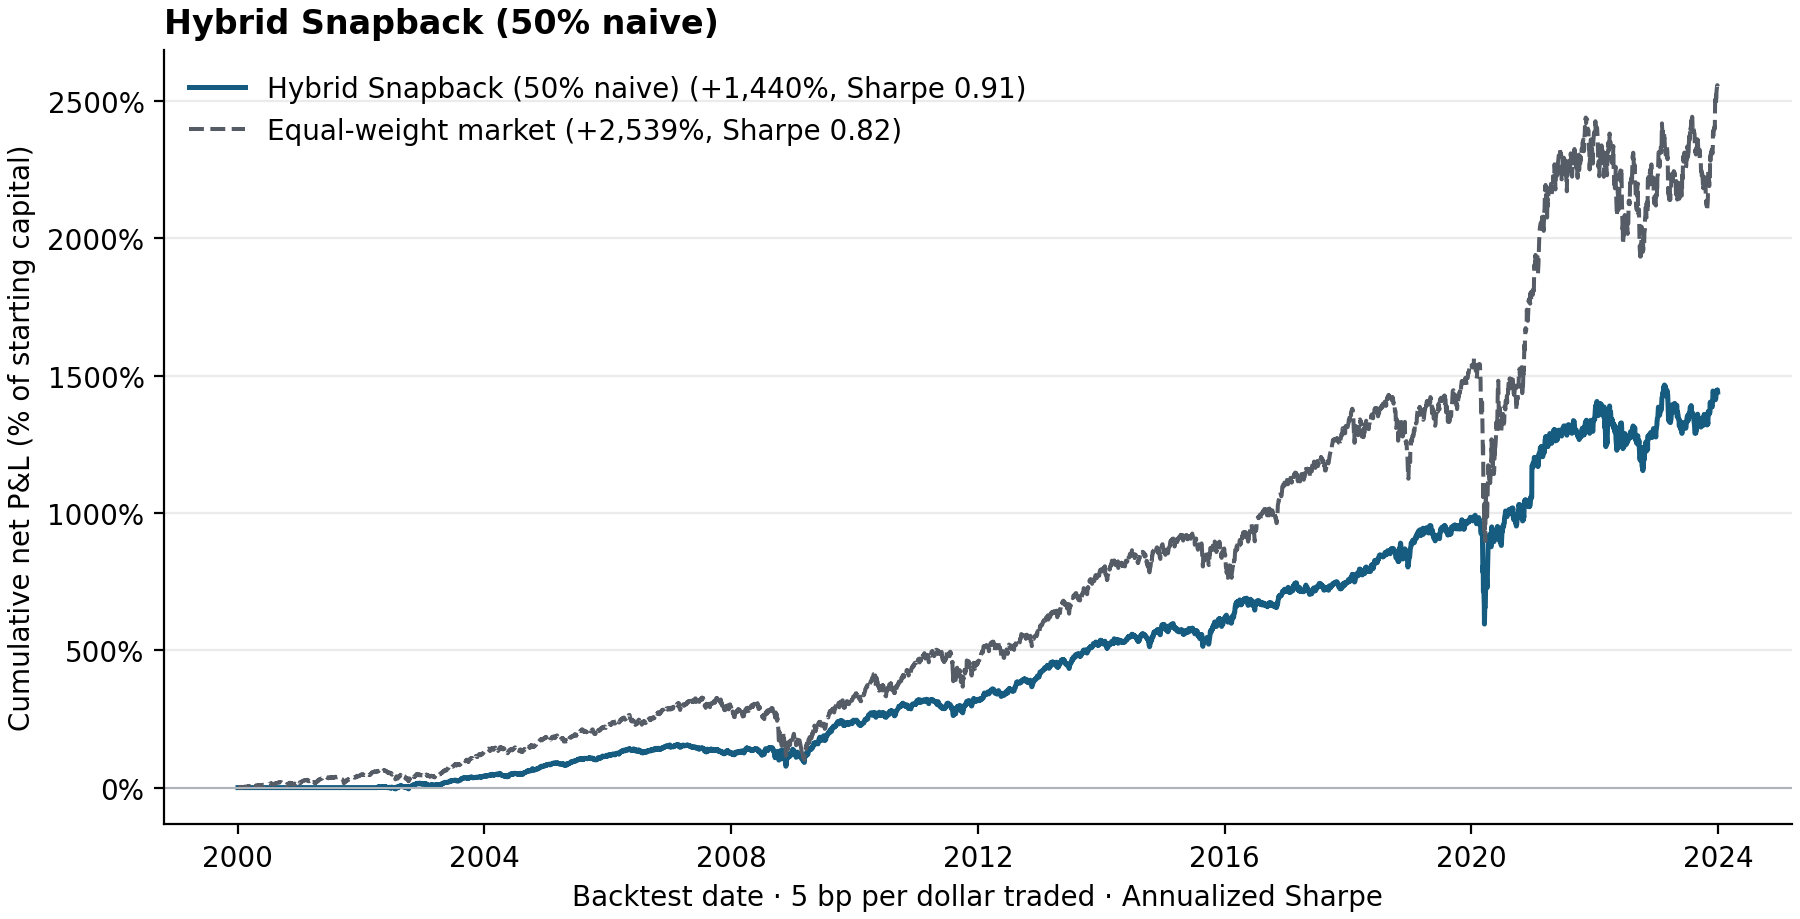
\includegraphics[width=0.5\linewidth]{50percentnaive_50hedged.png}
% ARCHIVE     \caption{50 percent naive and 50 percent hedged}
% ARCHIVE     \label{fig:placeholder}
% ARCHIVE \end{figure}
% ARCHIVE 
% ARCHIVE \begin{figure}[H]
% ARCHIVE     \centering
% ARCHIVE     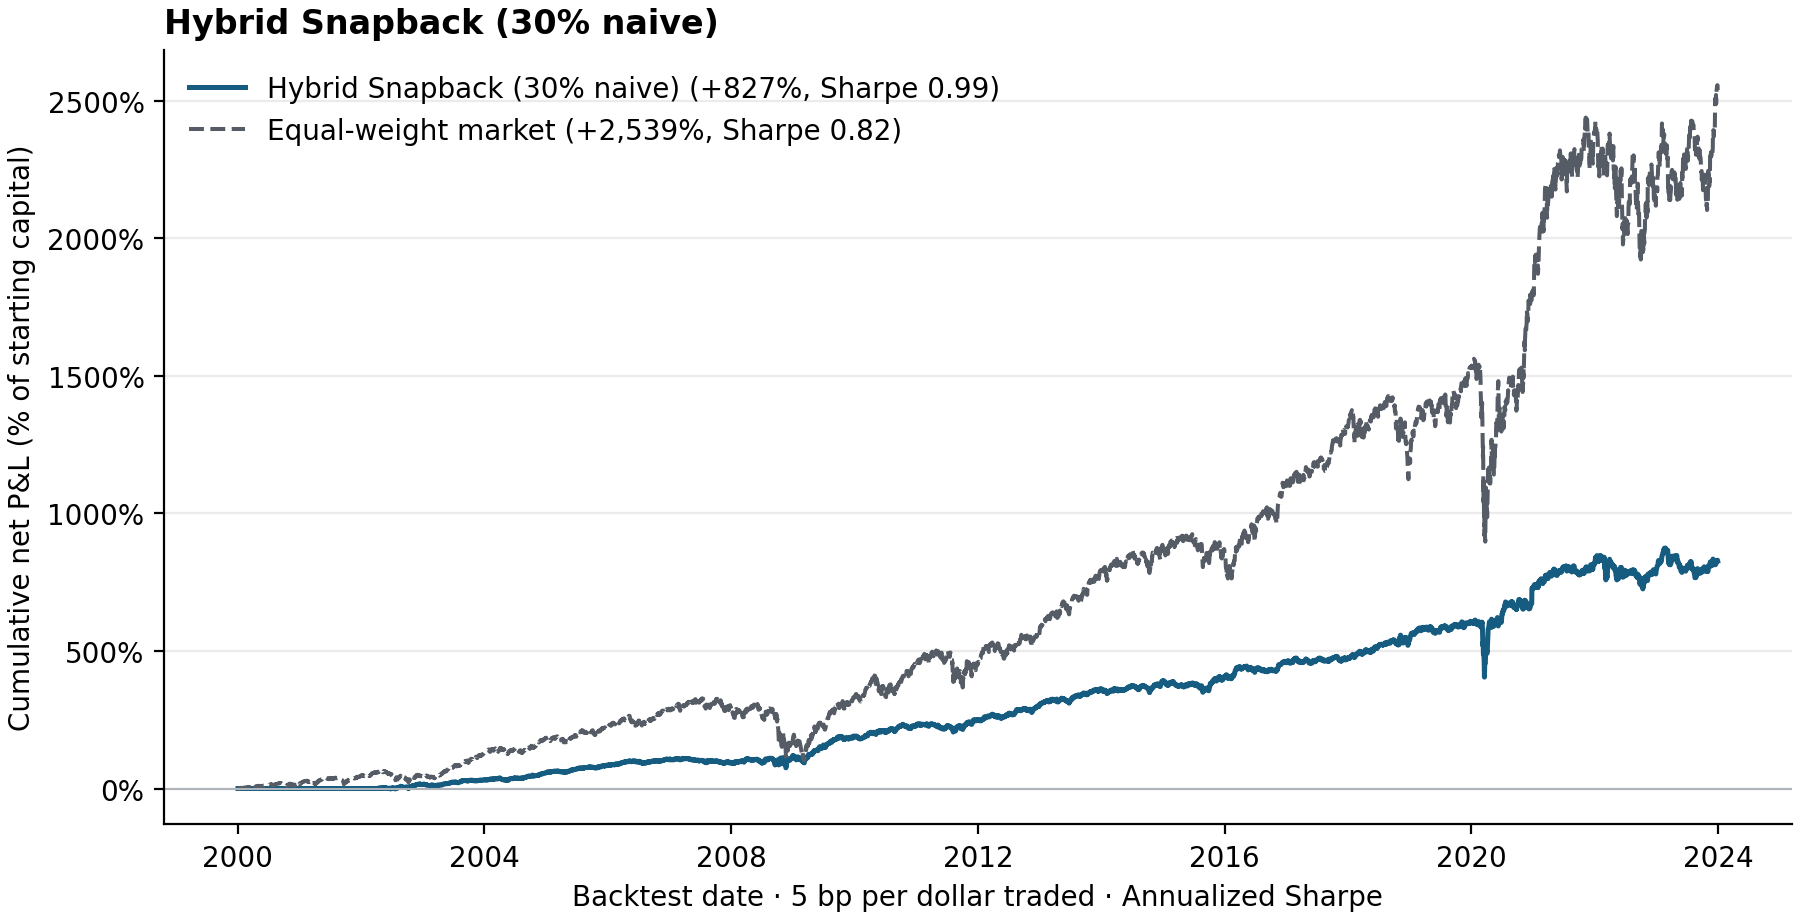
\includegraphics[width=0.5\linewidth]{30percentnaive.png}
% ARCHIVE     \caption{30 percent Naive + 70 percent hedged strategy}
% ARCHIVE     \label{fig:placeholder}
% ARCHIVE \end{figure}
% ARCHIVE 
% ARCHIVE \begin{figure}[H]
% ARCHIVE     \centering
% ARCHIVE     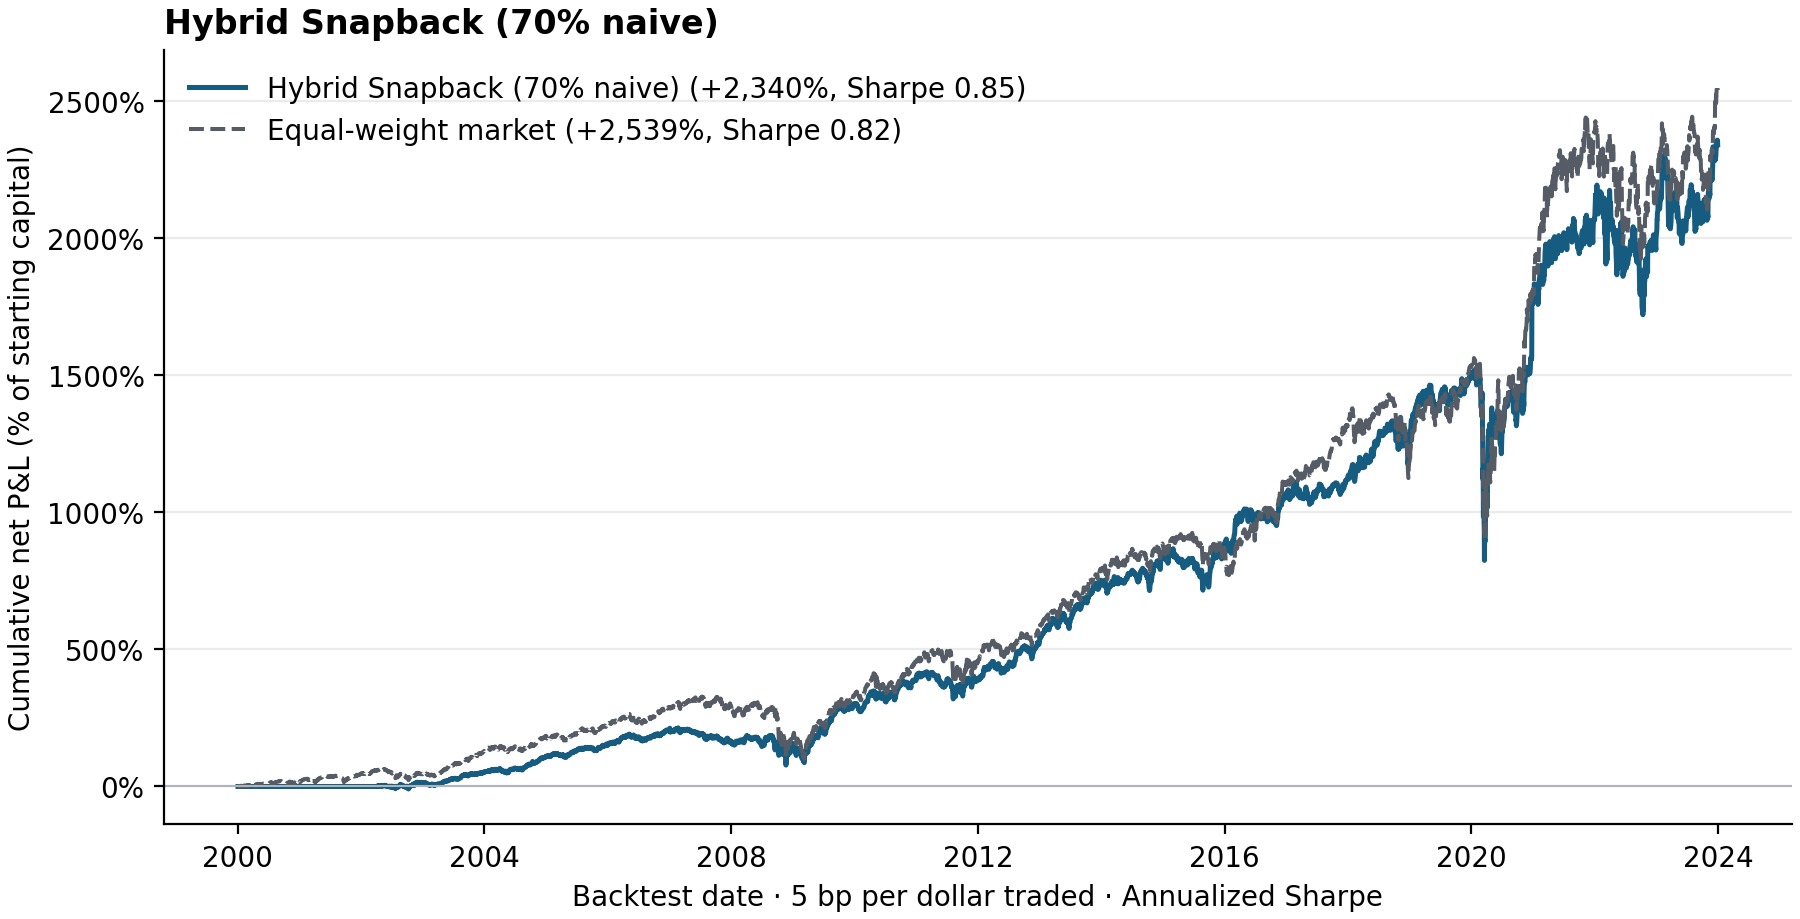
\includegraphics[width=0.5\linewidth]{70percentnaive_30percenthedged.png}
% ARCHIVE     \caption{70 percent naive and 30 hedged }
% ARCHIVE     \label{fig:placeholder}
% ARCHIVE \end{figure}
% ARCHIVE 
% ARCHIVE \paragraph{Volatility-weighted hybrid residual snapback.}
% ARCHIVE 
% ARCHIVE Note that in the fixed-weight hybrid strategies, we are supposed to choose a value of 
% ARCHIVE and keep this parameter the same throughout the trading horizon. Note that this may not be the ideal way to construct this strategy. For example, if we are in an uncertain time where stocks will tend to move around a lot, then it is better to have a portfolio that is more hedged to these risks. However, if we believe that stocks have lower volatility and that the tail risk of a particular asset class/sector/principal component dropping sharply in value, we are willing to take a more aggressive holding of stocks. 
% ARCHIVE 
% ARCHIVE We plan on changing this parameter depending on the volatility of the stocks. 
% ARCHIVE 
% ARCHIVE The first thing that we do is we calculate an equal-weight market return by averaging stock returns across our entire csv file for each day. (Essentially we calculate the return of the  equal weight market portfolio). Then, we can also estimate the sample standard deviation of these returns based off a specific set of returns. Thus, to estimate daily market volatility for each date t, we measure the sample standard deviation of these returns over the trailing 30 trading days. Note that this estimate uses only returns that are available by day t. 
% ARCHIVE 
% ARCHIVE After we do this, we let the variable pt[0,1] be the
% ARCHIVE resulting historical percentile rank of volatility. For example, if this is the lowest volatility in all of the history, then we would let pt be 0. However, if this was a the highest volatility, then we would let pt be 1. 
% ARCHIVE 
% ARCHIVE We will now use this pt value as the weight of our portfolio that we would like to have in the fully hedged portfolio. In other words, the weight on the naive portfolio is t=1-pt. 
% ARCHIVE 
% ARCHIVE Notice that the following hedged allocation for the weights are: 
% ARCHIVE 
% ARCHIVE \begin{figure}[H]
% ARCHIVE     \centering
% ARCHIVE     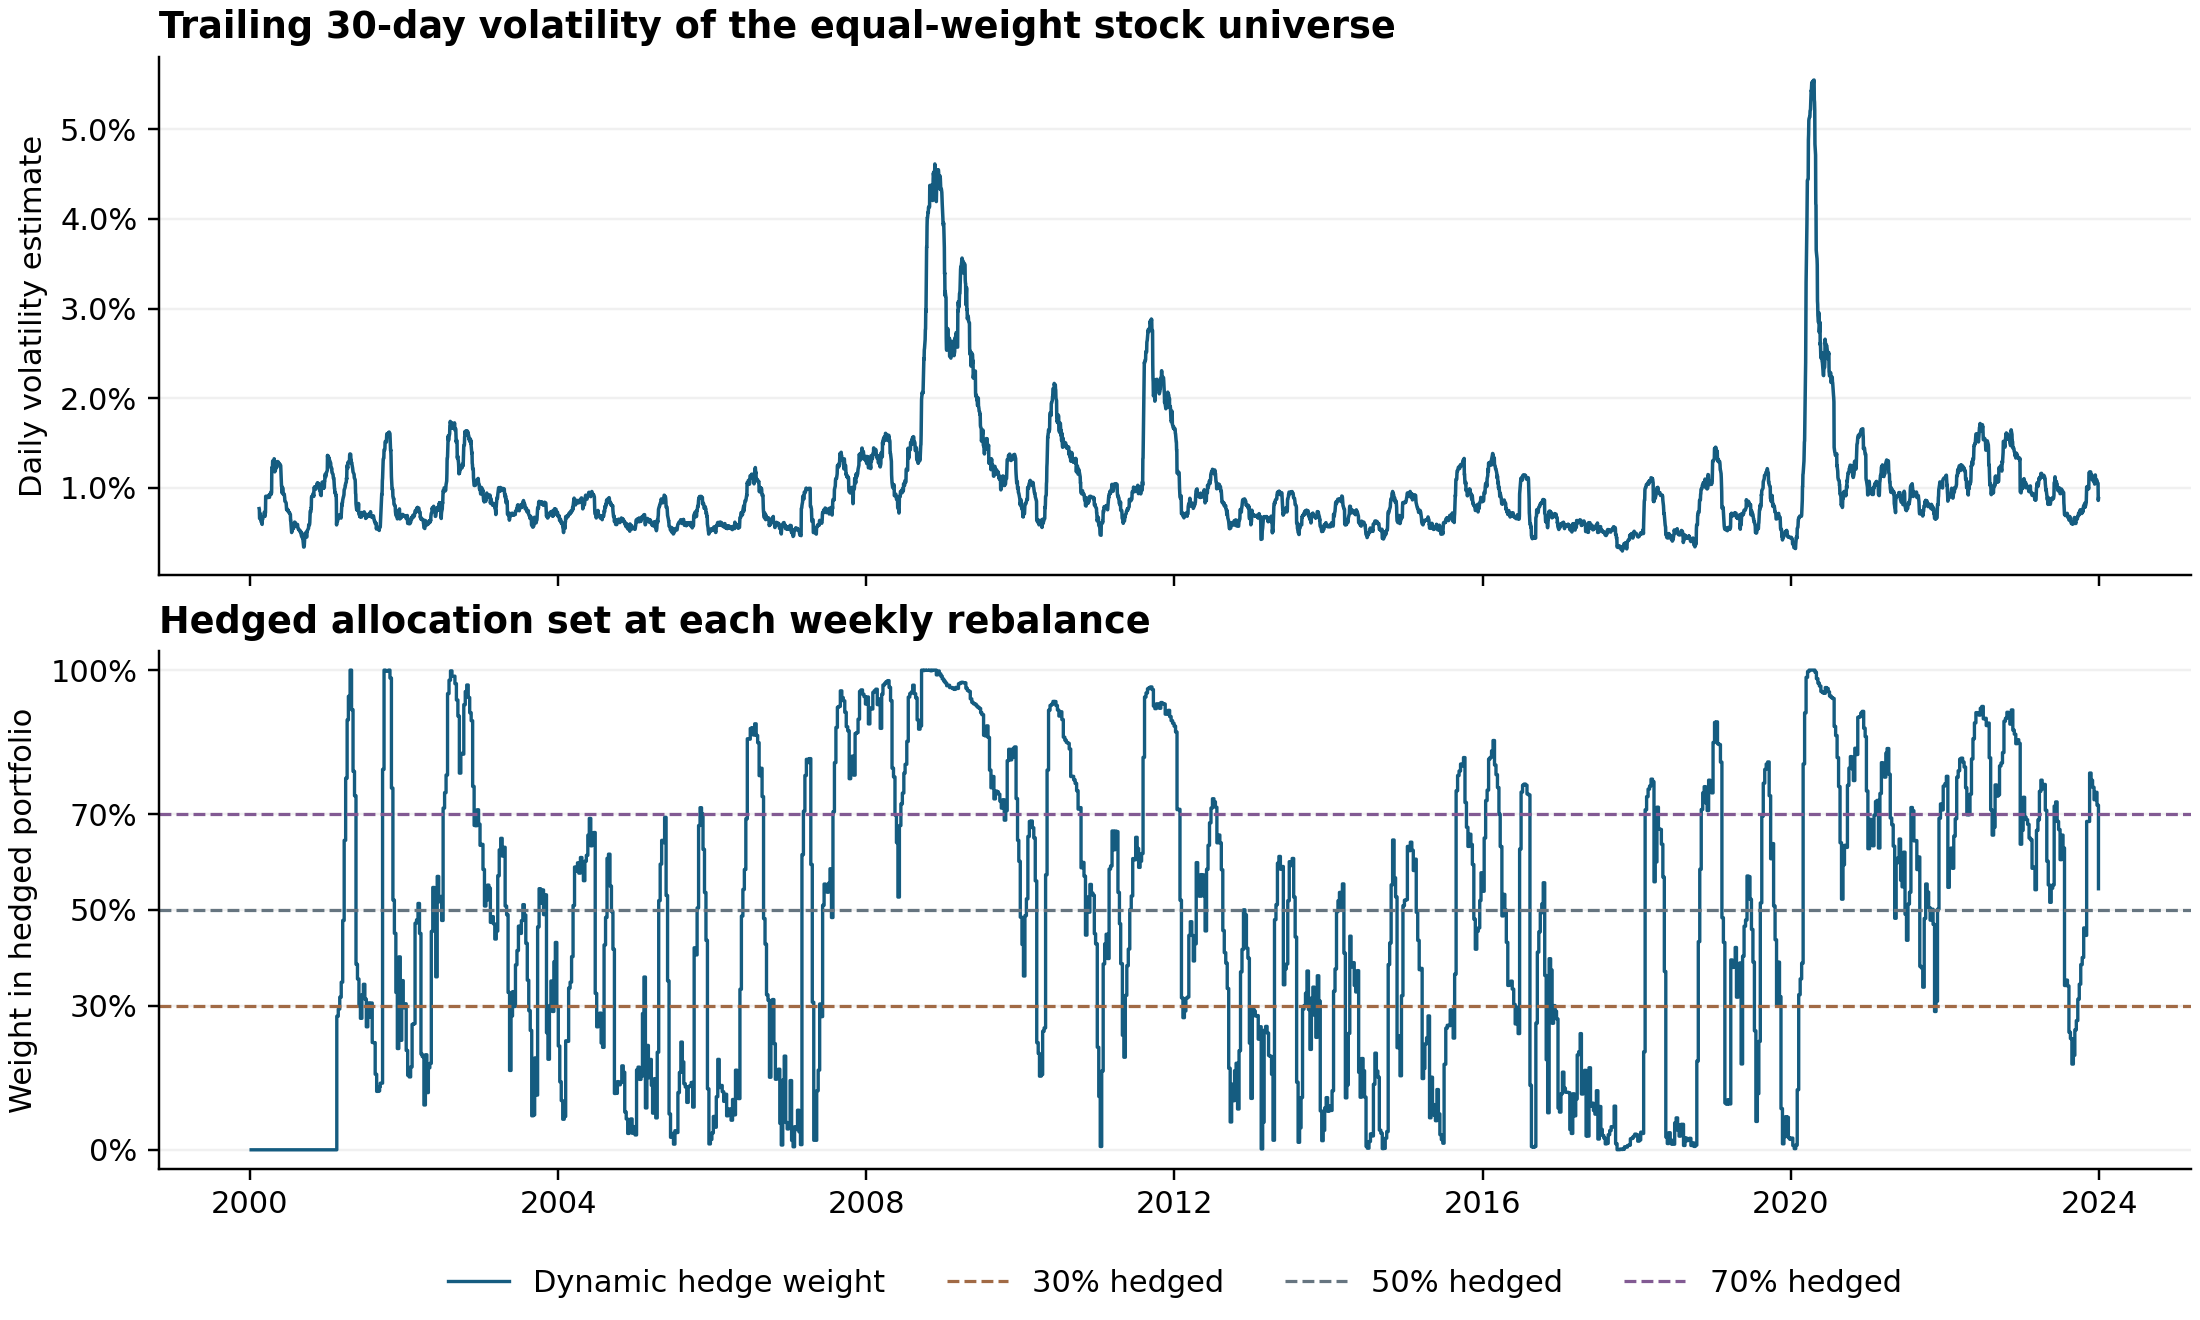
\includegraphics[width=0.5\linewidth]{volatility_allocation.png}
% ARCHIVE     \caption{Weight allocation based off volatility}
% ARCHIVE     \label{fig:placeholder}
% ARCHIVE \end{figure}
% ARCHIVE 
% ARCHIVE Although this graph looks pretty good, something to notice is that at the beggining of the timeline, we are alternative from 0 percent to 100 percent in the weights. This is because the rank is very sensitive to the few data points that we have. For example, at the beggining of this process we would have a sparse amount of data (for example the first data point is both the lowest and the highest volatility seen yet, so it is hard to factor this information into the model). 
% ARCHIVE 
% ARCHIVE 
% ARCHIVE To avoid this problem of letting a small number of early observations drive the allocation, we can use a symmetric Laplace smoothing to our weight allocation. 
% ARCHIVE Before each weekly re balance, we compare the current estimate of volatility with all earlier 30-day volatility estimates. 
% ARCHIVE We define the following variables: nt
% ARCHIVE be the number of earlier readings and kt be the number
% ARCHIVE below the current reading, with ties counting as 1/2. 
% ARCHIVE 
% ARCHIVE Then, we will add 126 pseudo-readings on each side of our current estimate. This gives us the following weight on the hedged portfolio:
% ARCHIVE \[
% ARCHIVE     \widetilde p_t = \frac{k_t+126}{n_t+252}.
% ARCHIVE \]
% ARCHIVE 
% ARCHIVE Note that now, with no earlier readings, the rule starts at a 50/50 mix. The starting mix receives weight of 252/(nt+252), so its "bias" decreases as more observations accumulate. For example, with 252 earlier readings, a raw volatility percentile of 90\% becomes a hedge weight of 70\%, halfway between the raw percentile and the 50\% starting weight.
% ARCHIVE 
% ARCHIVE The final portfolio allocates $\widetilde p_t$ to the fully hedged
% ARCHIVE portfolio and $1-\widetilde p_t$ to the naive portfolio:
% ARCHIVE \[
% ARCHIVE     \mathbf{w}_t^{\mathrm{dynamic}}
% ARCHIVE     =
% ARCHIVE     (1-\widetilde p_t)\mathbf{w}_t^{\mathrm{naive}}
% ARCHIVE     +
% ARCHIVE     \widetilde p_t\mathbf{w}_t^{\mathrm{hedged}}.
% ARCHIVE \]
% ARCHIVE 
% ARCHIVE Below is an image depicting the new weight allocation graph: 
% ARCHIVE 
% ARCHIVE \begin{figure}[H]
% ARCHIVE     \centering
% ARCHIVE     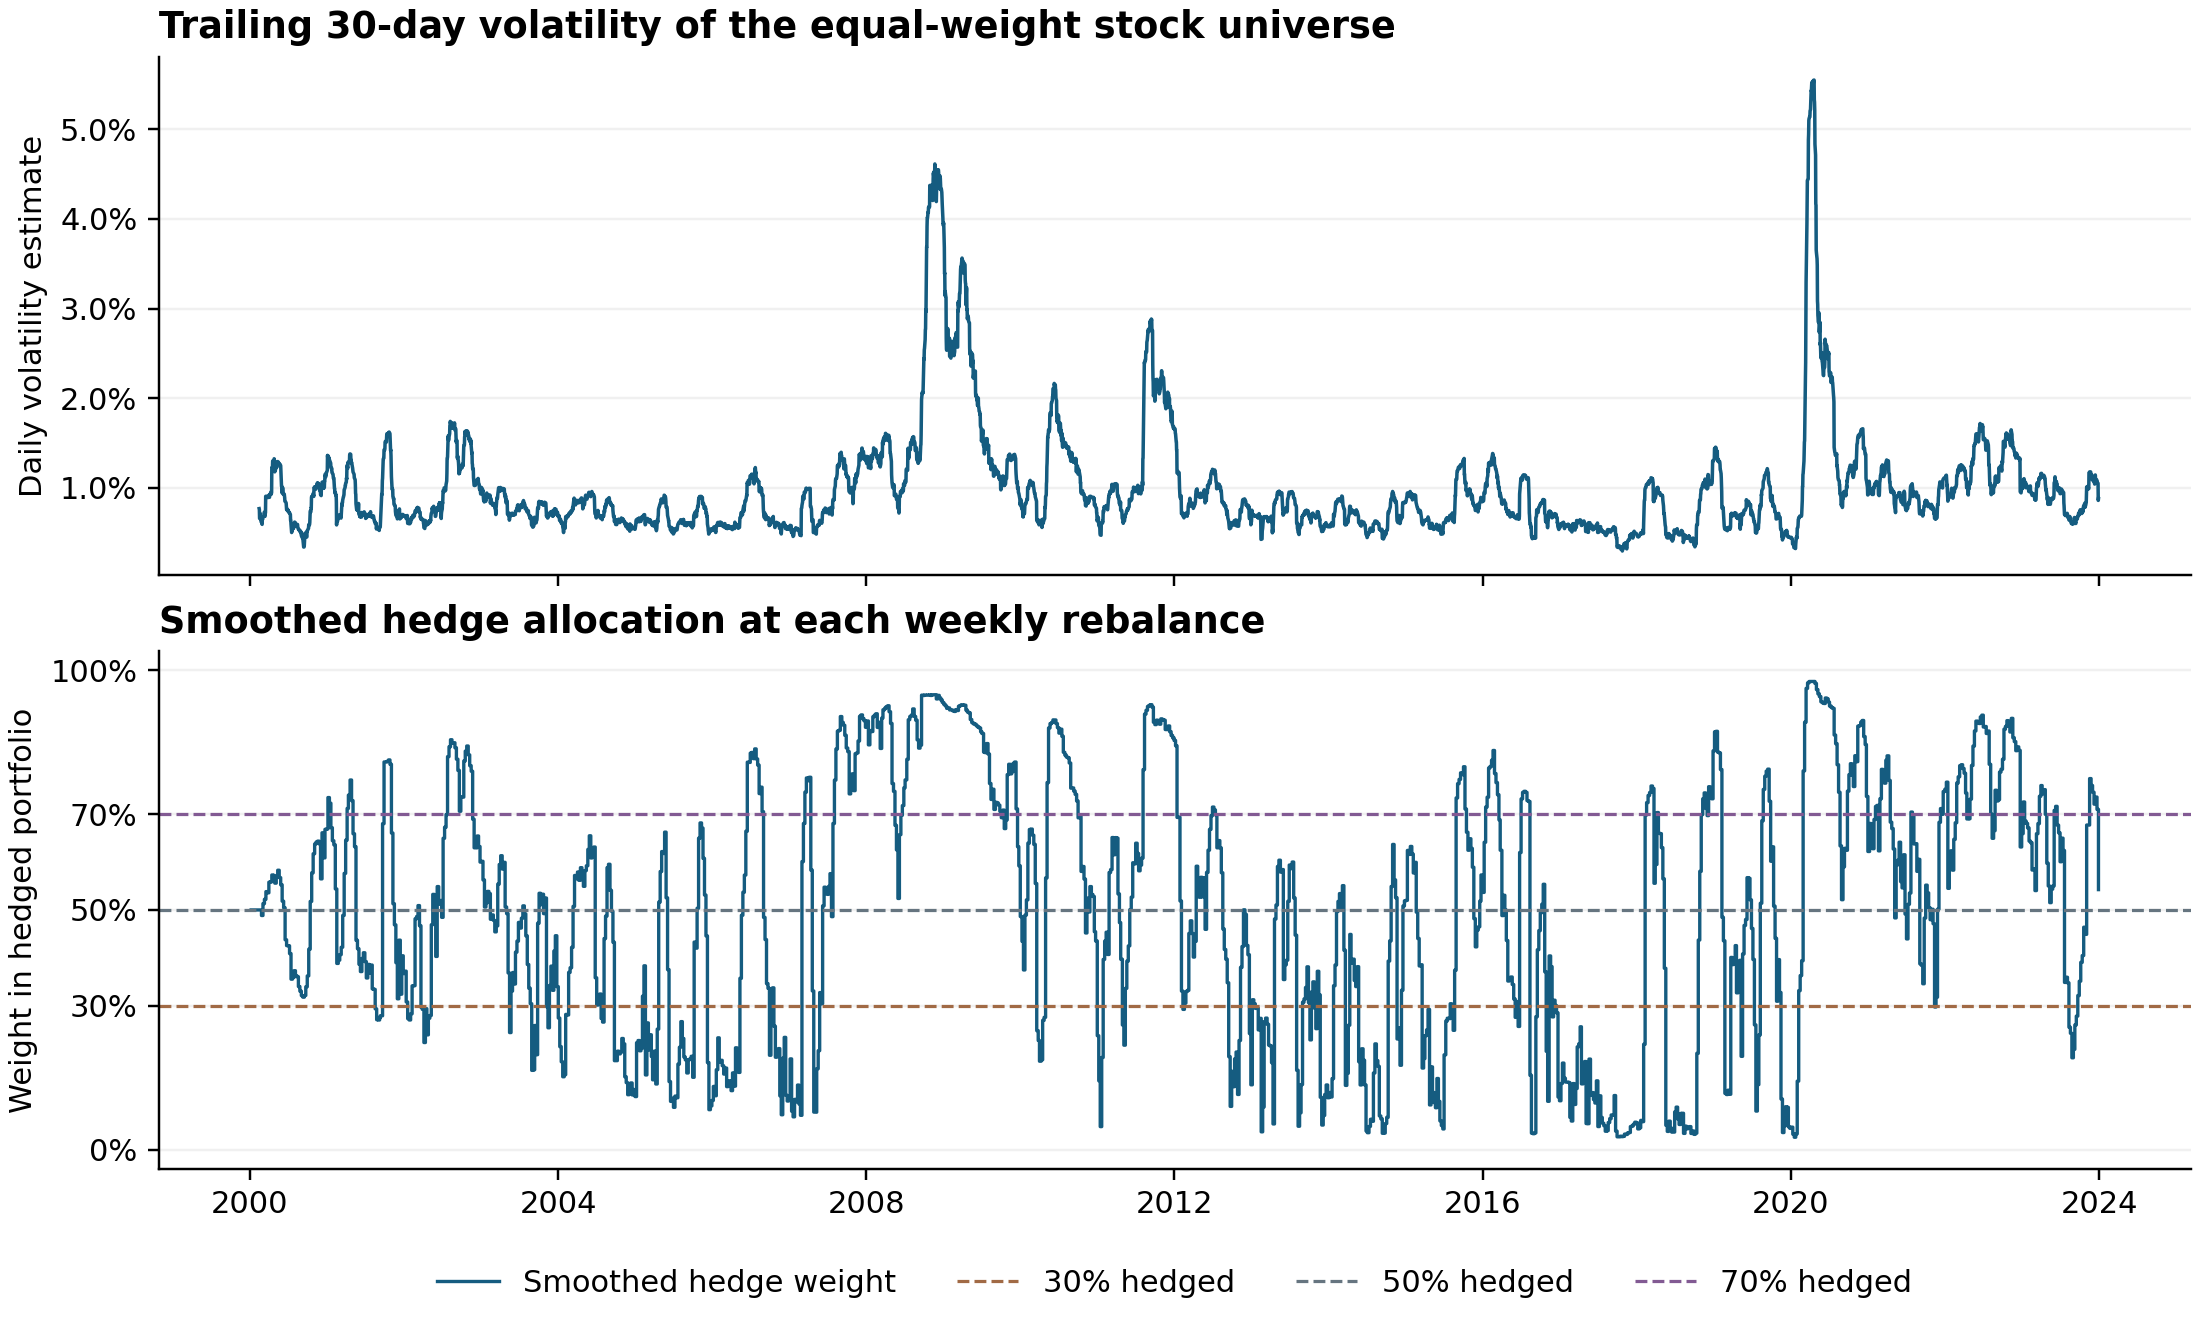
\includegraphics[width=0.5\linewidth]{updated_vol_weights.png}
% ARCHIVE     \caption{Enter Caption}
% ARCHIVE     \label{fig:placeholder}
% ARCHIVE \end{figure}
% ARCHIVE 
% ARCHIVE Implementing this strategy, we get the following results: 
% ARCHIVE 
% ARCHIVE \begin{figure}[H]
% ARCHIVE     \centering
% ARCHIVE     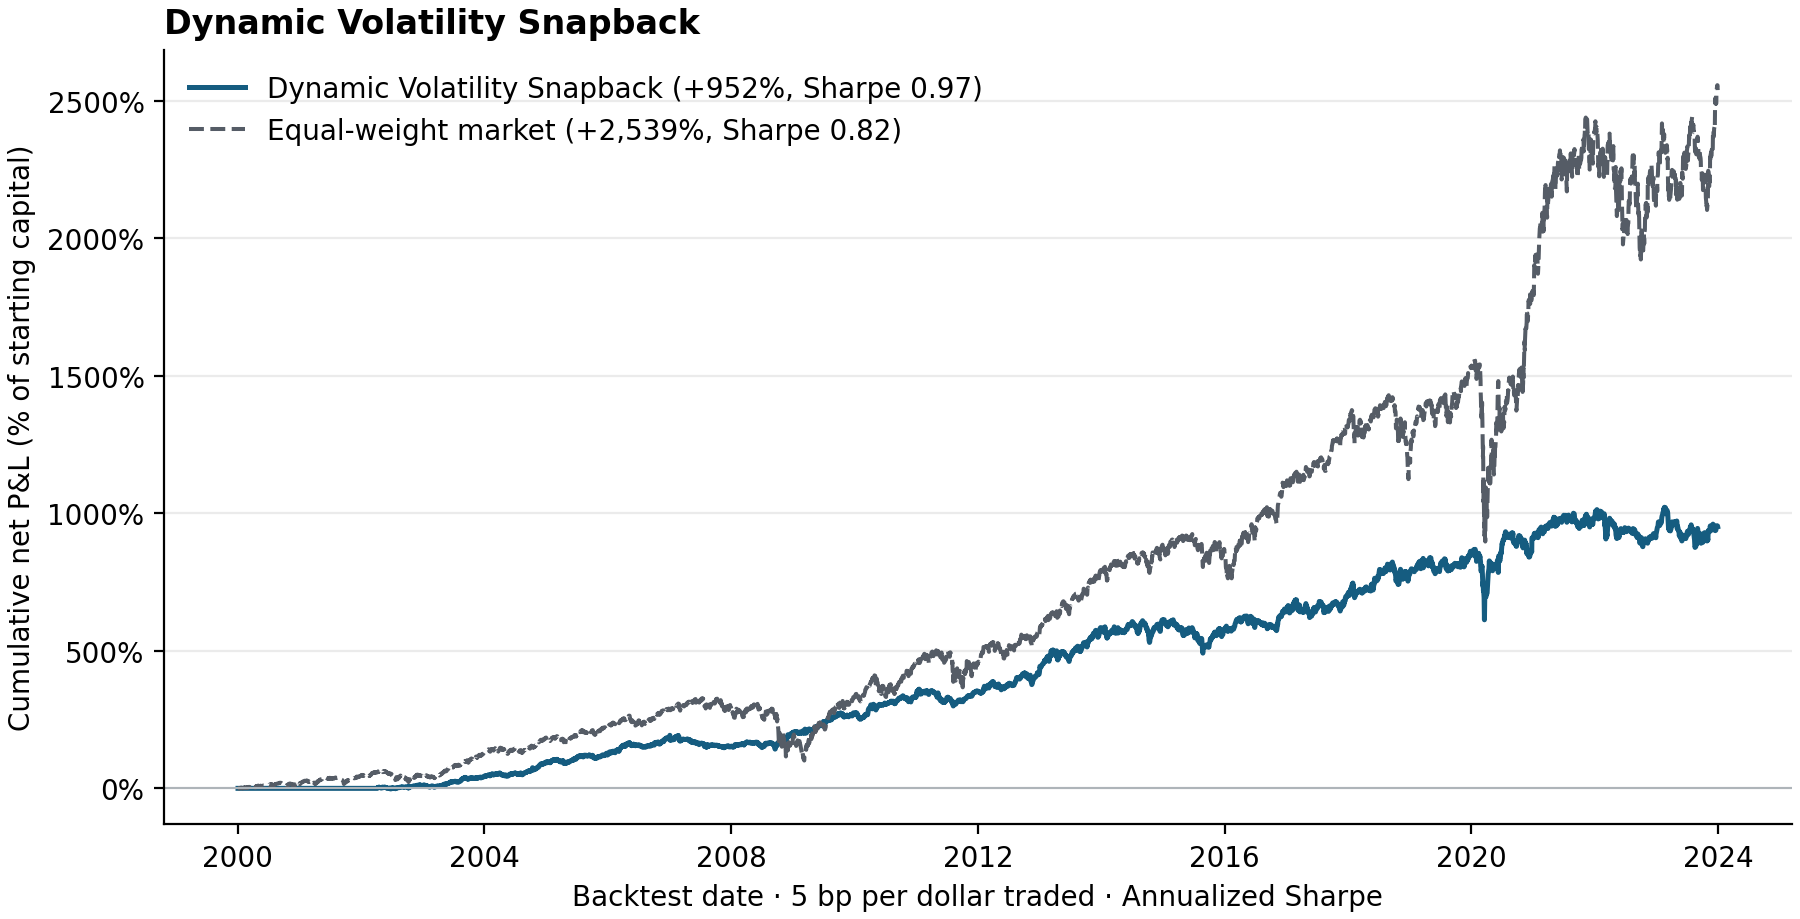
\includegraphics[width=0.5\linewidth]{dynamic_volatility.png}
% ARCHIVE     \caption{Dynamic Volatility PNL}
% ARCHIVE     \label{fig:placeholder}
% ARCHIVE \end{figure}
% ARCHIVE 
% ARCHIVE \subsection{Cumulative residual reversion}
% ARCHIVE 
% ARCHIVE The Residual Snapback strategy that we have been working on looks for stocks that have underperformed their
% ARCHIVE estimated factor exposures over the last three trading days. 
% ARCHIVE 
% ARCHIVE 
% ARCHIVE However, what if a stock is underperforming for a while and is drifting away from the market price, but then trades in line with the market for the three days that we are examining? 
% ARCHIVE 
% ARCHIVE In this case, the Snapback score could be very close to zero but the sum of all the culmulative residuals could be quite low. 
% ARCHIVE 
% ARCHIVE %hello 
% ARCHIVE The PCA factors that we have recieved are estimated from a previous past 500 day windw while the regression that we are fitting on has been trained over the past 100 days. A day's residual $\varepsilon_{i,t}$ is the difference between the stock's realized
% ARCHIVE return and the return explained by the fitted factor model (as discussed above in our naive strategy/the ones the followed).
% ARCHIVE 
% ARCHIVE For this strategy, we add every single daily residual to a total sum:
% ARCHIVE \[
% ARCHIVE     X_{i,t} = X_{i,t-1} + \varepsilon_{i,t}.
% ARCHIVE \]
% ARCHIVE 
% ARCHIVE Then, we compare the residual with how the residual has normally looked over the past 60 days (similar to how we have also normalized the residuals). 
% ARCHIVE \[
% ARCHIVE     z_{i,t}
% ARCHIVE     =
% ARCHIVE     \frac{X_{i,t}-\overline{X}_{i,t}^{(60)}}
% ARCHIVE          {s_{i,t}^{(60)}}.
% ARCHIVE \]
% ARCHIVE \begin{figure}
% ARCHIVE     \centering
% ARCHIVE     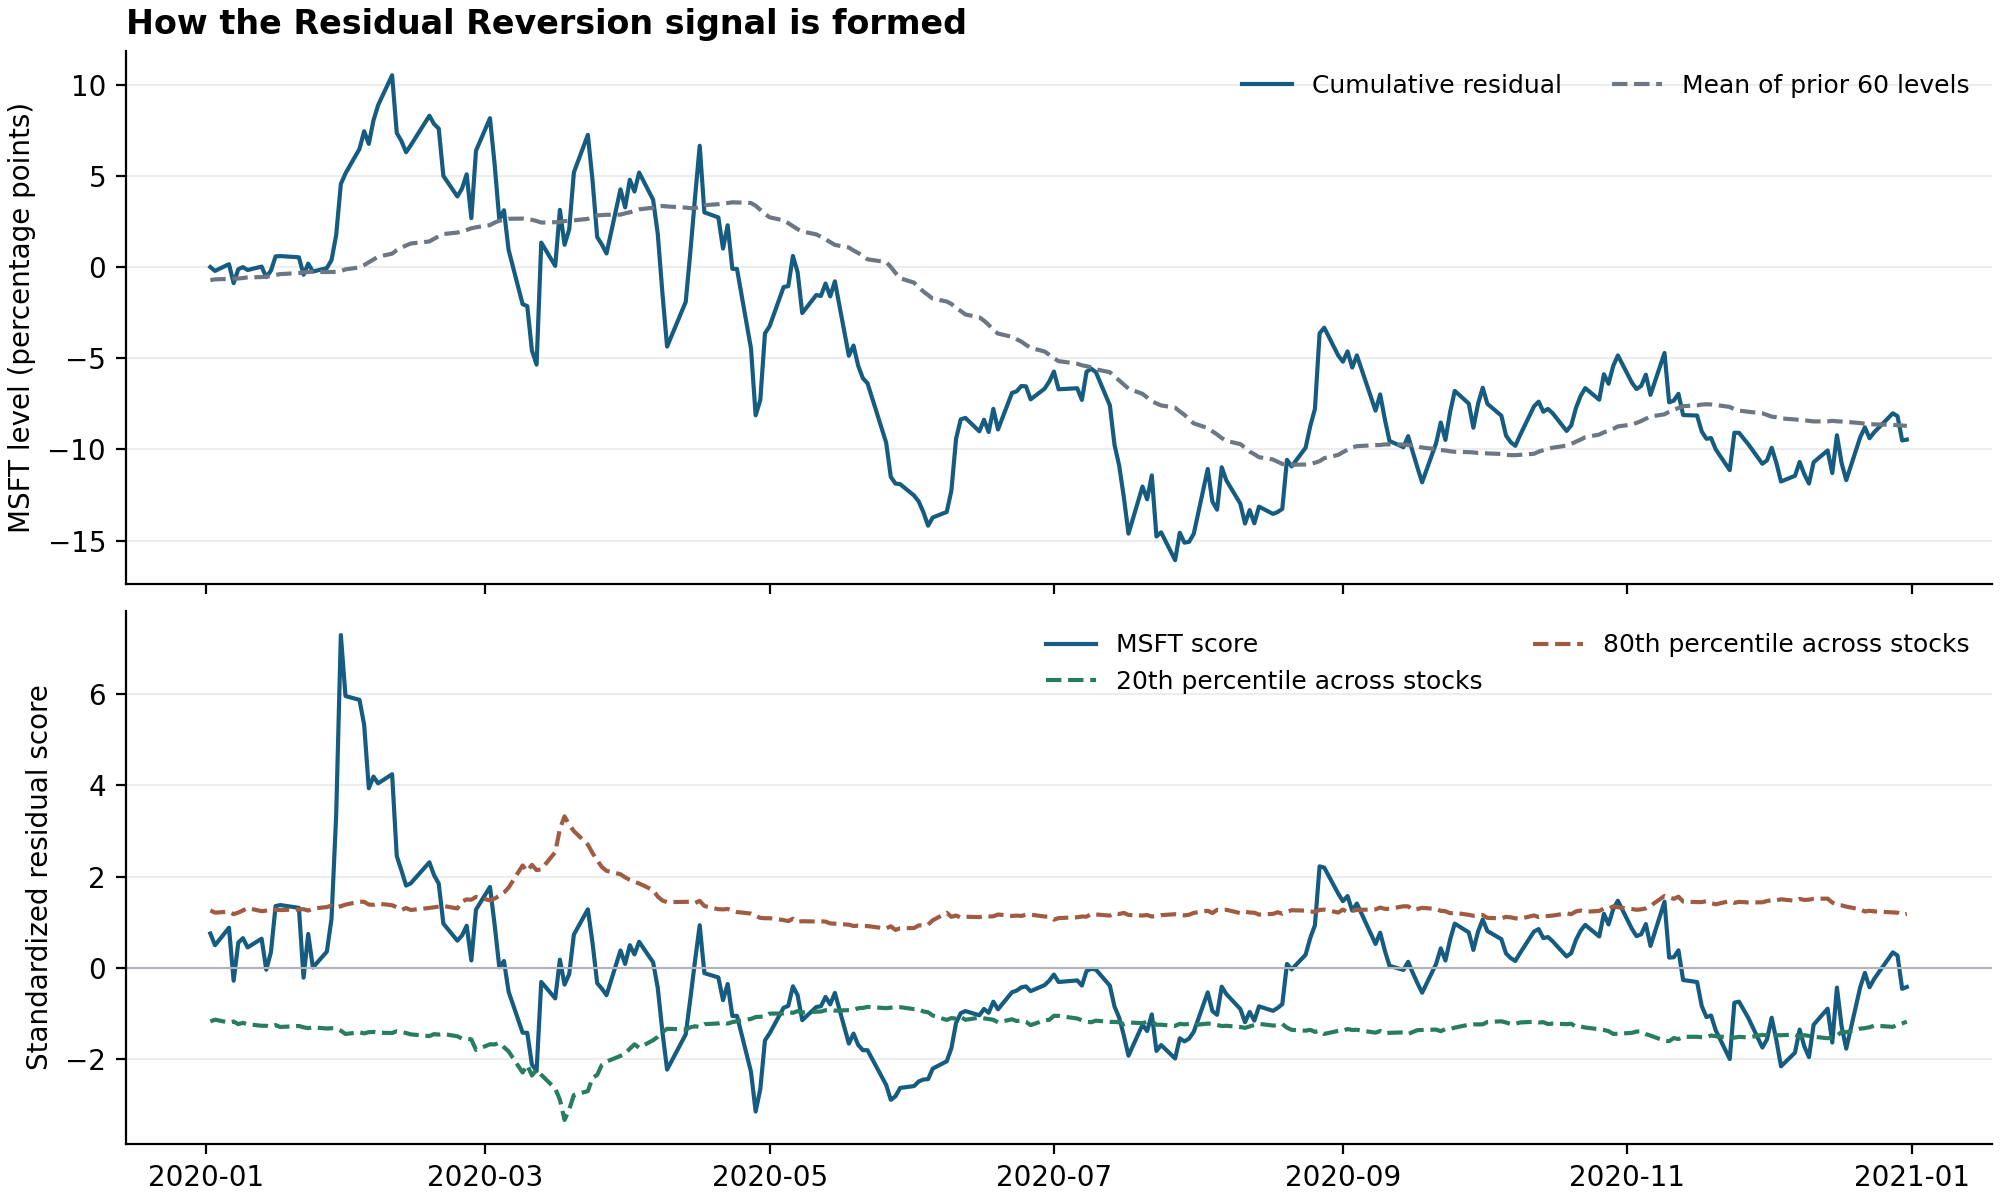
\includegraphics[width=0.5\linewidth]{msft_residual_reversion.png}
% ARCHIVE     \caption{Enter Caption}
% ARCHIVE     \label{fig:placeholder}
% ARCHIVE \end{figure}
% ARCHIVE 
% ARCHIVE Essentially, the way that the portfolio is made is we rank the stocks by their scores (as we have normally done for the other methods) and we buy the lowest-scoring 20\% and short the highest-scoring 20\%. This is slightly different than the naive method since we are account for a percent change rather than a strict cuttoff that we had in the naive method. 
% ARCHIVE 
% ARCHIVE 
% ARCHIVE Note that similar to the PCA factor neutral (fully hedged) strategy, we will ensure that our portfolio has zero estimated exposure to any of the 5 pca factors. We also want zero dollar exposure as well. So, the following two constraints is what we are up against: 
% ARCHIVE \[
% ARCHIVE     \mathbf{1}^{\top}\mathbf{w}_t=0,
% ARCHIVE     \qquad B_t\mathbf{w}_t=\mathbf{0},
% ARCHIVE \]
% ARCHIVE where the columns of $B_t$ contain the selected stocks' factor
% ARCHIVE loadings. The adjustment can shrink a position to zero while
% ARCHIVE preserving its direction. Individual weights are capped at 2\%
% ARCHIVE in absolute value. The neutrality constraints can leave some
% ARCHIVE capital unallocated, so gross exposure can fall below 100\%.
% ARCHIVE The backtest applies the current day's returns to existing
% ARCHIVE positions before placing the new trades.
% ARCHIVE 
% ARCHIVE 
% ARCHIVE 
% ARCHIVE 
% ARCHIVE 
% END ARCHIVED: Earlier residual-strategy draft; integrated treatment is in Section 4
\end{document}
